\documentclass[defaultstyle,11pt]{comps}

\usepackage{amssymb}		% to get all AMS symbols
\usepackage{graphicx}		% to insert figures
\usepackage[breaklinks]{hyperref}		% PDF hyperreferences??
\usepackage{breakcites}
\usepackage{longtable}
\usepackage{booktabs}
\usepackage{amsmath}
\usepackage[all]{nowidow}
\usepackage[section]{placeins}
\usepackage{flafter}


\usepackage{hyperref}
\hypersetup{
    colorlinks,
    citecolor=black,
    filecolor=black,
    linkcolor=black,
    urlcolor=black
}

\usepackage{floatrow}
\DeclareFloatFont{tiny}{\footnotesize}% "scriptsize" is defined by floatrow, "tiny" not
\floatsetup[table]{font=tiny}

\setkeys{Gin}{width=\maxwidth,height=\maxheight,keepaspectratio}

\providecommand{\tightlist}{%
  \setlength{\itemsep}{0pt}\setlength{\parskip}{0pt}}

\usepackage{natbib}
\bibliographystyle{plain}

\usepackage{graphicx}
\makeatletter
\def\maxwidth{\ifdim\Gin@nat@width>\linewidth\linewidth\else\Gin@nat@width\fi}
\def\maxheight{\ifdim\Gin@nat@height>\textheight\textheight\else\Gin@nat@height\fi}
\makeatother
% Scale images if necessary, so that they will not overflow the page
% margins by default, and it is still possible to overwrite the defaults
% using explicit options in \includegraphics[width, height, ...]{}
\setkeys{Gin}{width=\maxwidth,height=\maxheight,keepaspectratio}
% Set default figure placement to htbp
\makeatletter
\def\fps@figure{!htb}
\makeatother



\usepackage{float}
%\floatplacement{figure}{H}


\usepackage{longtable,booktabs}
\usepackage{calc} % for calculating minipage widths
% % % Correct order of tables after \paragraph or \subparagraph
% \usepackage{etoolbox}
% \makeatletter
% \patchcmd\longtable{\par}{\if@noskipsec\mbox{}\fi\par}{}{}
% \makeatother
% % Allow footnotes in longtable head/foot
% \IfFileExists{footnotehyper.sty}{\usepackage{footnotehyper}}{\usepackage{footnote}}
% \makesavenoteenv{longtable}
% 
\makeatletter
\AtBeginDocument{%
  \expandafter\renewcommand\expandafter\subsection\expandafter{%
    \expandafter\@fb@secFB\subsection
  }%
}
\makeatother

\setlength\parfillskip{0pt plus .75\textwidth}
\setlength\emergencystretch{1pt}

%%%%%%%%%%%%   All the preamble material:   %%%%%%%%%%%%

\title{Implementing Dynamic Foot Shape Models to Improve Spacesuit Boot Fit}

\author{Abhishektha}{Boppana}

\otherdegrees{B.S., Case Western Reserve University, 2017 \(\\\) M.S., University of Colorado Boulder, 2019}

%%\otherdegrees{B.A., North Dakota State University, 2005 \\
%%	      M.S., University of Reno, 2007}

\degree{Doctor of Philosophy}		%  #1 {long descr.}
	{Ph.D.~Aerospace Engineering Sciences}		%  #2 {short descr.}

\dept{Ann and H.J. Smead Department of}			%  #1 {designation}
	{Aerospace Engineering Sciences}		%  #2 {name}

\advisor{Dr.}				%  #1 {title}
	{Dr.~Allison P. Anderson}			%  #2 {name}

\reader{Dr.~Torin Clark}		%  2nd person to sign thesis

\readerThree{Dr.~David Klaus}		%  2nd person to sign thesis

\readerFour{Dr.~Rodger Kram}		%  2nd person to sign thesis

\readerFive{Dr.~Daniel Feeney}		%  2nd person to sign thesis

%%\readerThree{Thora Nea}		%  3rd person to sign thesis

\abstract{  \OnePageChapter	% because it is very short
	Abstract will be written in the future.
	
	}

%%\dedication[Dedication]{	% NEVER use \OnePageChapter here.
	
%%	}

%%\acknowledgements{	\OnePageChapter	% *MUST* BE ONLY ONE PAGE!
	
%%	}

\IRBprotocol{19-0071}	% optional!

\ToCisShort	% use this only for 1-page Table of Contents

%\LoFisShort	% use this only for 1-page Table of Figures
\emptyLoF	% use this if there is no List of Figures

%\LoTisShort	% use this only for 1-page Table of Tables
\emptyLoT	% use this if there is no List of Tables

%%%%%%%%%%%%%%%%%%%%%%%%%%%%%%%%%%%%%%%%%%%%%%%%%%%%%%%%%%%%%%%%%
%%%%%%%%%%%%%%%       BEGIN DOCUMENT...         %%%%%%%%%%%%%%%%%
%%%%%%%%%%%%%%%%%%%%%%%%%%%%%%%%%%%%%%%%%%%%%%%%%%%%%%%%%%%%%%%%%

\begin{document}
\begin{center}\rule{0.5\linewidth}{0.5pt}\end{center}

\hypertarget{chapter:motiv}{%
\chapter{Motivation}\label{chapter:motiv}}

The Apollo missions represent the last time humans set foot on another planetary surface, the Moon.
Future human spaceflight missions are retargeting planetary surface exploration by sending astronauts back to the Moon and onward to Mars.
While robotic missions can perform many of the scientific aspects of planetary exploration, human exploration still plays a key role in planetary mission success \citep{Drake2010}.

Spacesuits are designed to both provide life support and help protect the astronaut during activities conduced outside a space habitat, known as extravehicular activity (EVA).
EVA is an important consideration of planetary exploration, allowing astronauts to perform scientific experiments, collect geological samples, perform habitat maintenance, and construct infrastructure.
During EVA, astronauts are subject to many physiological and environment factors, including reduced gravity loading, dust, radiation, and extreme environment temperatures.
In addition, the lack of atmosphere does not provide life support.
Therefore, an EVA spacesuit's primary design objectives are to protect its operator from the environment and allow them to perform EVA tasks.

Humankind's current planetary EVA experience is limited to a total of 78 hours over 6 Apollo surface missions \citep{Portree1997}.
During the Apollo missions, astronauts performed almost 10 hours of EVA in a 24 hour period without the assistance of a rover during Apollo 14, and 22 hours of EVA in a 36-hour period with the assistance of a rover during Apollo 17 \citep{Portree1997}.
The longest traverse performed on the lunar surface occurred during Apollo 12, where astronauts Charles Conrad and Alan Bean walked 1.8 km \citep{Portree1997}.
Apollo 15-17 missions involving a rover assumed astronauts would be able to walk 5 km in case of rover failure \citep{Portree1997}, but this requirement is doubled for future missions.
Future planetary mission design assumes astronauts can walk up to 10 kilometers to return
to their habitat, and that astronauts can perform 8-hour EVAs, with a limit of 12 hours of EVA per 24 hours and 24 hours of EVA per 7 days \citep{Drake2010}.
In addition, NASA's current planetary exploration plans focus on extended stays and colonization, increasing surface mission time and therefore increasing total EVA time.
Future planetary EVA missions will therefore need a spacesuit that comfortably protects astronauts while they perform EVA tasks and traverse across the surface on these long duration missions.

\hypertarget{emu-spacesuit-injury-incidence}{%
\section{EMU Spacesuit Injury Incidence}\label{emu-spacesuit-injury-incidence}}

Following the Apollo era, space missions have all occurred in low Earth orbit in a microgravity environment.
New spacesuits, such as the Extra-Vehicular Mobility Unit (EMU) were designed for microgravity operations.
This included greater upper-torso mobility while reducing lower-torso mobility, as astronauts would be floating in space and not be required to ambulate.
However, the increase in EVA activities that accompanied the construction of the International Space Station have increased the incidence rates and severity of crew injuries, prompting studies into the human-spacesuit interactions and deficiencies in suit design that lead to these injuries.

Crewmember difficulties with the spacesuit have existed since the first EVA, where Alexi Leonov had difficulties moving the suit to re-enter the spacecraft.
Apollo astronauts have commented on the fatiguing reduced mobility of their spacesuits \citep{Scheuring2008}.
Gas pressurized spacesuits are known to be inherently stiff and rigid \citep{Parry1966, Abramov1994, Schmidt2001a, Holschuh2009}, difficult to move \citep{Norcross2009, Amick2015}, and have the potential to cause injuries both during operations and ground-based training \citep{Williams2003, Strauss2004, Scheuring2008, Scheuring2009, Anderson2015a, Chappell2017}.

The prevalence of injury has been well studied in the era of on-orbit microgravity EVAs performed with the EMU.
Strauss \citep{Strauss2004} found that 24.6\% of training sessions at the Neutral Buoyancy Laboratory (NBL) between 2004 to 2006 study had reported injury symptoms.
Viegas \citep{Viegas2004} found a 67.5\% reporting rate of injury symptoms from astronauts training in the NBL between 2002 to 2003.
An in-flight injury incidence of 0.24 was reported by Scheuring \citep{Scheuring2012} for EVAs occurring on Space Shuttle flights 90 to 113.
These injuries can be classified as contact injuries, including bruises and abrasions; and musculoskeletal injuries, including muscle tears, strains, and inflammation.

\hypertarget{spacesuit-contact-injuries}{%
\subsection{Spacesuit Contact Injuries}\label{spacesuit-contact-injuries}}

Spacesuit contact injuries have been the most reported operational injury mechanism in the US space program \citep{Scheuring2008}, and in the EMU \citep{Strauss2004, Viegas2004, Scheuring2012}.
Contact injuries occur through repeated contact between the wearer and the spacesuit.
High contact pressure between the wearer and spacesuit can lead to bruises, while shear can lead to abrasions \citep{Mailler2004, Carlson2006}.

EVA hand injuries have been reported since the Apollo era, with symptoms including swollen and abraded joints, putting the mission at risk \citep{Scheuring2012}.
Hand injuries continue to be most frequently reported injury in the EMU \citep{Strauss2004, Viegas2004, Scheuring2012}.
Hand contact injuries include fingernail delamination, abrasions, contusions, and nerve impingement \citep{Strauss2004, Viegas2004, Scheuring2012}.
These injuries have widely been attributed to the poor fit and unprotected contacts between the hand and the spacesuit glove \citep{Strauss2004, Viegas2004}.

Shoulder contact injuries occur from the combination of unprotected contact and high weight loading in the EMU \citep{Strauss2004, Viegas2004, Anderson2015a}.
Shoulder injuries are reported as the second most common EMU injury location and frequently occur during ground-based training in the NBL, when the wearer may be inverted in the suit \citep{Strauss2004, Viegas2004}.
While the suit and operator together are made neutrally buoyant, the operator is able to shift relative to the suit due to gravity.
Therefore, they ``fall'' into the suit, and are now making contact with the hard upper torso (HUT).
Therefore, the increased contact and high levels of load leads to shoulder contact injuries.

The feet are the next most reported areas of in-flight EMU contact injuries in the spacesuit \citep{Scheuring2012}.
Traditionally, not much motion occurs in the lower torso of the EMU spacesuit due to its design targeting microgravity operations.
The feet are normally restrained in a fixed foot restraint, while the astronaut performs tasks utilizing their upper body.
One astronaut reported a ``searing, knife-like pain'' on their foot during on-orbit EVA which was unable to be rectified \citep{Scheuring2012}.
This resulted in a blister and decreased sensation on the foot's dorsal surface, and was later attributed to having excess pressure bladder material in the boot \citep{Scheuring2012}.
Strauss \citep{Strauss2004} also reports contact injuries on the toes and dorsal surface stemming from the boot sizing insert, which does not adequately project the astronaut from contact from the foot restraint or bladder folds.

Other reported locations for EMU contact injuries include the elbow, knee, and trunk \citep{Strauss2004, Scheuring2012}.
Injuries at wearer's elbows and knees are reported to come from rubbing against the convolute joints \citep{Strauss2004}.
Injuries at the trunk are reported to occur from contact between the wearer's back and the Liquid Cooling and Ventilation Garment (LCVG) in the spacesuit \citep{Strauss2004}.

\hypertarget{spacesuit-musculoskeletal-injuries}{%
\subsection{Spacesuit Musculoskeletal Injuries}\label{spacesuit-musculoskeletal-injuries}}

Fatigue from high exertion may lead to musculoskeletal injuries
EMU Musculoskeletal injuries have been reported in the hands, due to the high exertion needed to actuate fingers on the pressurized glove \citep{Viegas2004}.
Fatigue may occur after many hours of completing EVA tasks \citep{Strauss2004, Scheuring2012}.
Similarly, the elbow joints in the EMU have also reportedly caused strains \citep{Strauss2004}.

Limitations of the EMU suit design can also lead to musculoskeletal injuries, the most severe which occurred at the shoulder \citep{Strauss2004}.
EMU operators can overuse their rotator cuff during EVA tasks, leading to muscle strains, sprains, tears, and overuse injuries \citep{Williams2003, Strauss2004, Strauss2005, Scheuring2012}.
Some of these injuries have required surgical intervention \citep{Strauss2005}.

\hypertarget{hypothesized-spacesuit-injury-mechanisms}{%
\section{Hypothesized Spacesuit Injury Mechanisms}\label{hypothesized-spacesuit-injury-mechanisms}}

Limitations in suit joint design and the poor fit between the suit and its operator can both lead to contact or musculoskeletal injuries.
While other environmental factors, such as increased humidity, were also found to have a role in EMU fingernail de-lamination \citep{Chappell2017}, this section will focus on the design and fit factors for spacesuits.
High exertion needed to actuate joints and poor indexing can lead to excessive musculoskeletal injuries, while poor sizing and poor indexing can lead to contact injuries, increasing the risk of injury fig.~\ref{fig:B-fitflow}.

\begin{figure}
\hypertarget{fig:B-fitflow}{%
\centering
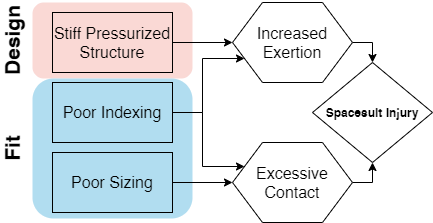
\includegraphics[width=0.6\textwidth,height=\textheight]{../fig/Background/fitflow.PNG}
\caption{Overview of how deficiencies in spacesuit design and fit can lead to increased injury risk}\label{fig:B-fitflow}
}
\end{figure}

Pressurized spacesuit joints require more energy to move than compared to unsuited motions \citep{Newman1997, Amick2015}.
While design features aim to reduce the effort needed to bend joints \citep{Harris2001}, these joints are difficult to engineer in areas such as the hand.
Therefore, the fatigue and strain injuries reported in the hand could be due to inherent design deficiencies of EMU spacesuit gloves \citep{Strauss2004, Viegas2004}.

Spacesuit joints also need to be properly aligned to the wearer to reduce both contact and musculoskeletal injury risk.
Indexing is a specific fit measurement regarding the alignment of the operator's joints to the spacesuit's joints.
Poor indexing can lead to contact injuries when suit-operator joint centers become misaligned and cause rubbing against the suit during motion, as seen in the elbow and knee of the EMU \citep{Strauss2004}. Deficiencies in suit design, including the high exertion to actuate joints and range-of-motion limitations, can also cause poor indexing and lead to injury.
Viegas reports a specific mechanism in the EMU glove where the high exertion required to actuate the glove results in dorsal displacement of the metacarpophalangeal joints, pushing the tops of fingers against the surface of the glove and causing inflammation \citep{Viegas2004}.
Poor indexing at the the EMU HUT design forces internal rotation of the shoulder due to the scye opening not allowing for full range-of-motion of the shoulders, leading to potential overuse and injury of the rotator cuff muscle \citep{Williams2003, Strauss2004, Strauss2005, Scheuring2012}.
Suit joints should therefore be designed and sized to ensure proper indexing.

Suit components also need to be properly sized to the operator to reduce contact injury risk.
Sizing, along with indexing, ensures that the suit is fit to the operator.
Spacesuits in the Apollo era were custom tailored to each astronaut.
However, as the astronaut corp grew, the EMU presented a modular sizing system, where differently-sized suit components had to be selected for each astronaut.
Gaps between the wearer and the spacesuit could lead to excessive contact when the wearer moves and shifts inside the spacesuit \citep{Benson2009}.
Suit components which are too small can also cause higher contact pressures, leading to potential contact injuries \citep{Anderson2015b}.
Poorly sized bladder inserts were found to be a factor in EMU foot injuries \citep{Strauss2004}. Opperman et al. \citep{Opperman2010} found that higher hand circumferences have a larger incidence of fingernail delamination in the spacesuit glove, while Charvat et al. \citep{Charvat2015} found smaller hand circumferences to be a risk factor in fingernail delamination, showing how sensitive fit is in leading to injury.
Suit components should therefore be sized accurately to the suit's operator to ensure proper fit.

\hypertarget{spacesuit-injury-countermeasures}{%
\section{Spacesuit Injury Countermeasures}\label{spacesuit-injury-countermeasures}}

Attempts to mitigate spacesuit injury have focused on addressing the fit and mobility limitations of the EMU.
Newer spacesuit prototypes feature larger scye openings for better indexing and more mobile shoulder bearings compared to the EMU \citep{Graziosi2016}.
However, testing of microgravity EVA task performance in the NBL found that while the new design allowed for more shoulder compatibility, larger subjects still reported discomfort in the shoulder area \citep{Meginnis2018}.
This shows how sizing and indexing are just as important as spacesuit mobility to ensure a properly compatible spacesuit.
It still remains impossible to perfectly fit every person to the EMU spacesuit due to the wide ranges of anthropometry and limited sizing components \citep{Benson2009}.
Back padding on the EMU was found to potentially assist wearers in controlling the upper torso of the suit, reduce over-rotation of the torso to keep upper extremity joints aligned, and improve indexing at the gloves \citep{Chappell2017}.
For wearers with a smaller anthropometry however, indexing at the hip bearings was unable to be fixed by padding, due to the limitations in torso length.
In addition, effects of indexing on performance are inconclusive \citep{Fineman2018}.
Therefore, there is a need to improve spacesuit sizing and indexing to work with any improvements in spacesuit mobility to reduce the risk of contact and musculoskeletal injuries.

\hypertarget{summary}{%
\section{Summary}\label{summary}}

The push towards planetary exploration requires advancements in spacesuit design to create a safe and comfortable environment for astronauts to perform EVAs.
Our planetary exploration experience is limited to just 6 Apollo missions to the Moon as missions have shifted towards microgravity research, but future plans call for an extended human presence on the Moon and Mars.
Microgravity EVAs and training have resulted in many upper torso injuries due to hard-to-move joints and poorly fitted suits.
The transition to planetary EVAs, with a focus on ambulation, may result in a higher incidence rate of injuries in the lower torso without significant changes in the way spacesuits are designed and fitted.
Therefore, it is important to understand how operator-spacesuit interactions and spacesuit performance may lead to injury in the context of planetary tasks such as ambulating as planetary surface missions are planned.
This will allow for the construction of safer and more comfortable spacesuits to reduce the risk of injuries during EVA.

\hypertarget{background}{%
\chapter{Background}\label{background}}

Poor suit design and suit fit are two of the main suit variables leading to injury risk and compromised performance during EVA \citep{Chappell2017}.
Pressurized spacesuits will continue to be used for EVAs through the transition from microgravity to planetary exploration, and therefore will require improvements to their joint design and fit to ensure safe and comfortable EVA.
As future missions target planetary exploration, ambulating across the surface becomes a critical EVA task, and requries an understanding of reduced-gravity ambulation and suited effects on ambulation.
There are also many challenges that are associated with fitting spacesuits which have not yet been solved.
This chapter introduces how current suits perform in planetary ambulation and introduces the challenges with fitting spacesuits.

\hypertarget{planetary-ambulation}{%
\section{Planetary Ambulation}\label{planetary-ambulation}}

Walking is not always the most energetically preferable gait.
Astronauts during the Apollo missions did not walk while traversing the surface; they famously loped across the surface.
In fact, loping is the energetically preferred gait on the Lunar surface, while walking, skipping, and running are energetically preferable on Mars \citep{Ackermann2012b}.
As speeds increase in lunar gravity, a transition occurs from walking to skipping rather than from walking to running as on Earth \citep{Minetti2012}.
However, the energetically preferred speed is not always achievable or possible, and slower walking speeds may be necessary when performing EVA tasks.

Studying the walk-run or walk-skip transition gives further insight into ambulation on a planetary surface.
Walking is modeled as an inverted pendulum which conserves some energy between each step; but energy is not conserved at faster walking speeds and needs muscular power input \citep{Cavagna1976, Cavagna1977}.
Griffin et al. \citep{Griffin1999} found as gravity is reduced, the amount of mechanical energy conserved between each step is reduced, and the maximum energy recovery occurs at slower speeds.
Ivanenko et al. \citep{Ivanenko2002} found that muscle activation and ground contact forces decreased with lower gravity levels, but kinematic coordination of the lower limbs were not affected by gravity levels.
The Froude number is the ratio between the centripetal and gravitational forces in the inverted pendulum model, as shown in eq.~\ref{eq:froude}.
\begin{equation}\protect\hypertarget{eq:froude}{}{
Fr=\frac{v^{2}}{gL}
}\label{eq:froude}\end{equation}

Where \(Fr\) is the Froude number, \(v\) is the velocity of ambulation, \(g\) is the gravitational force, and \(L\) is the leg-length \citep{AlexanderMcN.1989}.
At some critical value, walking is theoretically impossible as the gravitational force cannot match the required centripetal force, which is where the walk-run transition occurs (\(Fr*\)).
Humans typically switch to running at \(Fr=0.5\).
Kram et al. \citep{Kram1997} offloaded subjects by their waist as they walked and ran on a treadmill, and found that \(Fr*\) increases at lower gravity levels.
The increase in \(Fr*\) was hypothesized to be from the arms and legs not being offloaded and still under the influence of gravity \citep{Kram1997}.
Donelan and Kram \citep{Donelan2000} also found that elastic forces were unable to predict the dynamics of reduced-gravity running.
This suggests that other factors may be at play with walking in reduced gravity.

Ambulating with the suit involves additional forces both applied by the suit, and applied by the user to control the suit.
Newman and Alexander \citep{Newman1993} suggested that energy may be expended at low speeds and lower gravity levels for stability and postural control for ambulation.
Chappell \citep{Chappell2006} found that when the offload system was set to lock waist rotation for stability, subject's gait was constrained and showed changes in braking and propulsion force for Lunar gravity.
Therefore, stability is an important factor in walking at lower gravity levels.

Carr and McGee \citep{Carr2009} developed the Apollo number \(Ap\) to explain the effects of the spacesuit's pressure forces on gait (eq.~\ref{eq:apollo}).

\begin{equation}\protect\hypertarget{eq:apollo}{}{
Ap = \frac{Fr}{M}\\
\textrm{,where $M$ is the mass ratio of the spacesuit.}
}\label{eq:apollo}\end{equation}

\(M\) encorporates the self-supported weight of the spacesuit.
The self-supported weight of the spacesuit is from the spacesuits pressurization.
Carr and McGee validated the Apollo number against gait events during Apollo missions, but found that the Apollo number did not fully explain the walk-skip transitions.
\emph{Therefore, a gas-pressurized spacesuit's mobility restrictions and joint mechanical work, along with its pressure forces, may also be affecting suited ambulation.}

\hypertarget{gas-pressurized-spacesuit-characteristics}{%
\section{Gas Pressurized Spacesuit Characteristics}\label{gas-pressurized-spacesuit-characteristics}}

\hypertarget{an-inherently-stiff-structure}{%
\subsection{An Inherently Stiff Structure}\label{an-inherently-stiff-structure}}

Gas pressurized spacesuits have been used for all EVAs throughout the history of human spaceflight.
However, gas pressurized suits become stiff and rigid when pressurized, requiring great effort to bend.
The first EVA spacesuit, the Gemini suit, did not include any design features to reduce bending effort \citep{Thomas2012}.
If a gas pressurized suit component is represented as a pressurized cylinder, bending the cylinder along its axis causes a reduction in volume at the bend \citep{Harris2001}.
As a result, pressure at the bend will increase, causing resistance to the bending force.
The force required to change the volume at the bend is presented in eq.~\ref{eq:press} \citep{Newman1997, Harris2001},
\begin{equation}\protect\hypertarget{eq:press}{}{
F = \frac{W}{d} = \frac{\frac{p\pi D^{3}\phi}{8}}{\frac{L\phi}{2}} = \frac{p\pi D^{3}}{4L}
}\label{eq:press}\end{equation}
where \(F\) is the force required, \(W\) is the work required, \(d\) is the distance the joint is flexed, \(p\) is the pressure, \(D\) is the cylinder's diameter, \(\phi\) is the joint deformation angle, and \(L\) is the length of the cylinder.
It can be seen that the force required to bend a pressurized joint is not dependent on the bending angle, but rather the length and diameter of the pressurized section.
Without dedicated mobility features to maintain a constant volume at joints, the forces required to bend representative spacesuit components can be as high as 200 lbs for the waist joint \citep{Newman1997}.

\hypertarget{mobility-design-features}{%
\subsection{Mobility Design Features}\label{mobility-design-features}}

Mobility design features allow for bending of a pressurized joint by creating a point at which the joint can buckle, and allowing the joint to maintain constant volume through the bending motion \citep{Harris2001}.
This greately reduces bending resistance and allows for joint flexibility \citep{Harris2001}.
These mobility features typically feature some form of bellows or convolutes to maintain constant volume and axial restraints to prevent elongation of the joint under pressurization \citep{Harris2001}.

Mobility design features have been studied and iterated since the advent of space travel, but were not implemented in the Apollo mission suits.
The Litton company built and tested spacesuits for EVA use in the 1950s, predating both the US and Russian space programs.
These suits iterated on the use of convolutes by inventing the rolling convolute, annular convolute, and cardonic hard joint \citep{Harris2001}.
While these suits never saw operations on spaceflight, they did prove benefits in mobility over the International Latex Corporation (ILC) designed A7L suits, which were eventually used by US astronauts on the moon.
The Litton suits were able to match the center of restraint and center of pressure when convolute joints were bent, reducing the bending torque and spring return force of the joint \citep{Harris2001}.
Therefore, the suit's operator is able to easily bend the joint and not exert much force to keep the joint bent.
The A7L suit's convolute joints did not match the center of restraint and center of pressure, requiring operators to exert additional force to both bend the joint and keep it bent \citep{Harris2001}.
Such drawbacks of the A7L suit required astronauts to come up with clever workarounds.
On an Apollo 16 EVA, astronaut John Young found that ``by hopping into the air and landing on his feet, the weight of his suit overcame the suit's internal pressure, so he could get to his knees and pick up rocks without using geological tools'' \citep{Portree1997}.
Integrating convolutes into the A7L suits may have improved mobility on the Moon.

Advancements since the Apollo era have brought us improvements in pressurized joint design to increase mobility, including the toroidal mobility joint, dual-axis joint, hard component joints, hybrid hard-component/fabric joints, and improvements to flat-patterned joints \citep{Harris2001}.
The Mark III Advanced Space Suit Technology Demonstrator EVA Suit (MK III) is a spacesuit designed by NASA as a planetary spacesuit design testbed \citep{Kosmo1988}.
These advancements have allowed for increased lower-torso mobility as shown in the MK III spacesuit technology demonstrator; operators are easily able to recover from a fall and kneel in the MK III while these tasks were done with much difficulty in the A7L and EMU spacesuits \citep{Kosmo1998}.

Lessons from EMU and MK III design were applied to the design of the new Z2 planetary spacesuit prototype.
The Z2 prototype was first developed by NASA and ILC Dover in 2016 to demonstrate planetary surface exploration technologies, but parts of the Z2 suit are now being used for the Exploration EMU (xEMU), to supplement or replace the EMU for ISS EVAs \citep{Graziosi2016, Meginnis2018}.
The Z2 also serves as the basis for the design of the Artemis spacesuits, which will be worn by the first crew to step foot on the Moon.
The Z2 spacesuit features a larger scye opening and more mobile shoulder bearings compared to the EMU \citep{Graziosi2016}.
Tests of the Z2 in the NBL found range-of-motion and reach envelope improvements over the EMU, but many microgravity EVA tasks were reported to be harder and more limited in the Z2 \citep{Meginnis2018}.
Subjects also reported similar muscle fatigue and exertion ratings between the EMU and Z2 \citep{Meginnis2018}.
Larger subjects also reported discomfort in the shoulder area, further highlighting the importance of fit in spacesuit design \citep{Meginnis2018}.
Similar analysis needs to occur with ambulation to assess the effect of suit mobility improvements.

\hypertarget{mk-iii-ambulation-performance}{%
\section{MK III Ambulation Performance}\label{mk-iii-ambulation-performance}}

The MK III spacesuit has been used to experimentally study suited effects on ambulation due to the Z2's relative novelty.
In the EVA Walkback Test (EWT), six male subjects were tested with the MK III spacesuit on a treadmill to explore the effects of the MK III spacesuit's weight on planetary ambulation in Lunar (1/6g) and Martian (3/8g) gravity levels.
Subjects were tested in three conditions: unsuited and offloaded to selected gravity level; unsuited and offloaded to selected gravity level with the suit weight matched; and suited while offloaded to selected gravity level \citep{Norcross2009}.
This allowed for analysis of suit weight separately from other suit design factors on the metabolic cost of suited ambulation.
Subjects were tested at three speeds above and three speeds below their walk-run transition speed.
All subjects also did a 1G baseline unsuited trial and a 10 km suited lunar ambulation.
A follow-on integrated suit test (IST) examined the effects of varied suit mass, gravity, and on metabolic cost and kinematics on Lunar suited gait \citep{Norcross2010} with similar conditions while varying suit pressure and mass.
These and similar tests provide insight into how the MK III's design factors affect suited ambulatory performance.

\hypertarget{cost-of-transport-factors}{%
\subsection{Cost of Transport Factors}\label{cost-of-transport-factors}}

Metabolic cost of transport, a measure of how much energy the body is exerting during ambulation calculated through direct calorimetry \citep{Kenny2017}, was collected in these tests across a variety of conditions.
Metabolic cost is a direct measure of how hard the body is working to move in the spacesuit.
Previous studies have shown that the metabolic cost of transport decreases with gravity \citep{Grabowski2005}.
Findings from the EWT and IST were consistent with these previous findings \citep{Norcross2009, Norcross2010}.
Unsuited weight-matched metabolic costs were lower than 1G unsuited across all speeds for 1/8G ambulation and similar to 1G unsuited for 3/8G ambulation \citep{Norcross2009}.
This suggests that without suit effects, ambulation on Mars may be metabolically similar to ambulating on Earth.
However, the MK III increased the metabolic cost of transport for both gravity environments compared to the unsuited weight-matched condition \citep{Norcross2009}.
At 1/6G, the MK III had a higher metabolic cost than Earth ambulation at lower speeds, but was less metabolically costly at higher speeds \citep{Norcross2009, Norcross2010}.
The MK III was very metabolically costly in 3/8G, metabolic cost quickly approach maximal values for low speeds and subjects were unable to run in the suit at higher speeds \citep{Norcross2009}.
The metabolic cost of weight (5\%-13\%) for both Lunar and Martian gravity levels was significantly dwarfed by the cost of suit design factors (87\%-95\%) \citep{Norcross2009}.
From these results, its apparent that the MK III's design cannot service ambulation on Mars due to its design factors, but may be sufficient for the Moon.

Other suit design factors partially explained the increased metabolic cost of suited ambulation.
The IST found increased suit pressure to minimally increase metabolic cost across all speeds, hypothesized to be due to the MK III's constant volume joints \citep{Norcross2010}.
However, there were some subjective differences in mobility noted across the different pressures, although there was no correlation to subject anthropometry \citep{Norcross2010}.
The effect of suit weight, which encompasses gravity level and suit mass, steadily increased with speed \citep{Norcross2010}.
The percentage of metabolic cost that was not explained by suit weight or pressure decreased as speed increased, but then increased at the fastest speed \citep{Norcross2010}.
Additional factors which can explain the increased metabolic cost can include suit kinematics, stability, and harnessing effects from the gravity offloading, which may be causing more difficulty for ambulation at lower speeds.
However, these factors were not isolated in the MK III ambulation experiments.
The majority of ambulation during an EVA is most likely done at lower speeds, thereby requiring further understanding of how suit design is affecting mobility at low speeds.

\hypertarget{ambulation-biomechanics}{%
\subsection{Ambulation Biomechanics}\label{ambulation-biomechanics}}

The IST captured little differences in kinematics as a function of pressure, which may be due to the constant volume joints \citep{Norcross2010}.
However, it was noted that at 4.3 psi, the knee joint was limited by the design of the pressurized suit, and that the ankle increased its range-of-motion (ROM) to compensate the limited knee ROM \citep{Norcross2010}.
This shows the importance of the kinematic chain in suited mobility; when a certain motion is inhibited, other joints along the kinematic chain will have to compensate.
Similar compensation has led rotator cuff injury in the EMU's HUT \citep{Williams2003}.

Cullinane et al. \citep{Cullinane2017a} found suited MK III ambulation at 1G to reduce heel and toe clearance above ground compared to unsuited ambulation.
In addition, the MK III was found to decrease speed, stride length, and step length compared to unsuited ambulation \citep{Cullinane2017a}.
Cadence and stance time increased with gravity level in the IST, consistent with how metabolic cost increases with gravity level \citep{Norcross2010}.
These findings suggest that the MK III inhibits operator mobility and agility when ambulating.

\hypertarget{subjective-feedback}{%
\subsection{Subjective Feedback}\label{subjective-feedback}}

Subjective feedback allows operators of the MK III to provide their perception of ambulating in the suit.
Rating of Percieved Exertion (RPE) and Gravity Compensation and Performance Scale (GCPS) were consistent with metabolic cost findings in both the IST and EWT; both increased with gravity and speed \citep{Norcross2009, Norcross2010}.
Subjects performing the 10 km suited lunar ambulation in the EWT reported ``fair'' to ``moderate'' operator compensation required to walk in the MK III on the Cooper-Harper Scale \citep{Norcross2009}.
While mean rating of discomfort was ``very low'' to ``low'' on the Corlett-Bishop Scale, discomfort and trauma were noted on the knees and feet of some subjects \citep{Norcross2009} (fig.~\ref{fig:B-Trauma}).
In addition, muscular fatigue and tightness was also reported in the quadriceps, thighs, glutes, and lower back \citep{Norcross2009}.

Subjective feedback for ambulating in the MK III at 1/6-g suggests that it is mostly acceptable for lunar ambulation.
However, the reported trauma and musculoskeletal discomfort are areas of concern.
The EWT and IST, along with findings from Cullinane et al. \citep{Cullinane2017a}, show that the MK III's design inhibits natural human motion and requires more effort during suited ambulation.
It is not enough, however, to design a suit that more closely matches natural human motion; it also needs to work closely with its operator to reduce injury risk from poor fit.

\begin{figure}
\hypertarget{fig:B-Trauma}{%
\centering
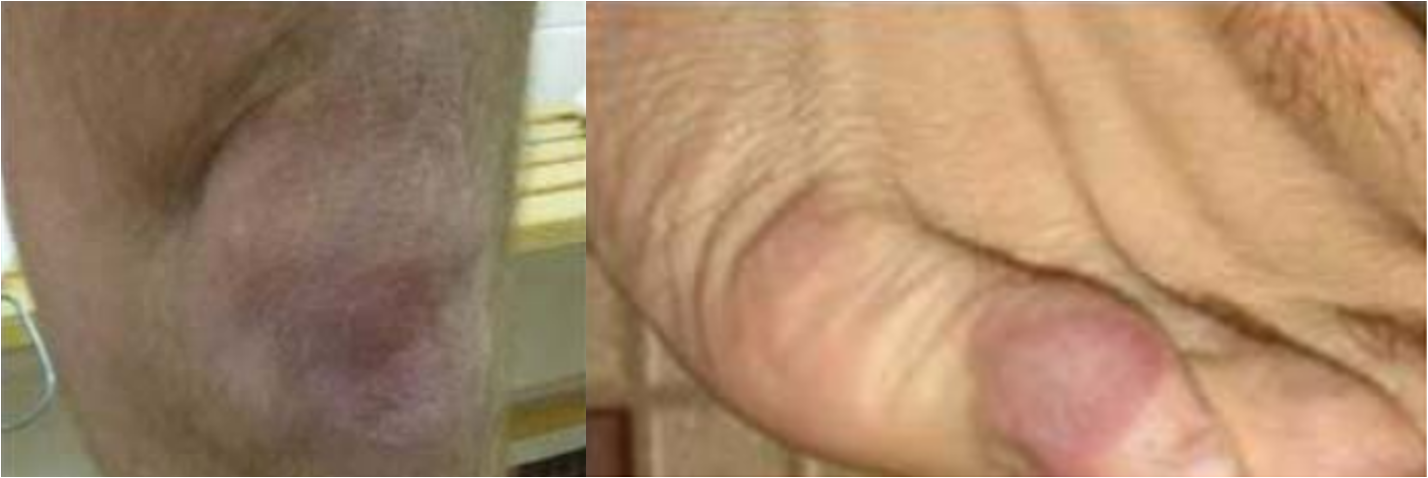
\includegraphics[width=0.8\textwidth,height=\textheight]{../fig/Background/Trauma.png}
\caption{Knee (left) and foot (right) trauma identified in the MK III following 10 km walkback evaluation. From Norcross et al.~2009}\label{fig:B-Trauma}
}
\end{figure}

\hypertarget{spacesuit-fit}{%
\section{Spacesuit Fit}\label{spacesuit-fit}}

Spacesuit mobility needs to have matched spacesuit-operator interaction, primarily driven by spacesuit fit, to ensure the suit works with its operator.
Proper spacesuit fit requires both correct sizing and correct indexing between the spacesuit and its operator.
In addition, these factors must be maintained not only in a static pose, but through dynamic movements as well.
Static fit refers to the alignment between the operator and the spacesuit, while dynamic fit refers to the coordination of the operator to the spacesuit during motions \citep{Stirling2020}.
Poor static fit leads to empty space around the operator, which allows the operator to move inside and repeatedly contact the spacesuit.
However, improving static fit is not as easy as filling this empty space; this would hamper operator mobility and lead to poor dynamic fit and difficulty for the operator to move the suit.
In addition, the effect of fit on suited performance is difficult to understand.
Difficulty in both sizing the suit and ensuring that suit movements match operator movements may be further improved through body shape modeling.

\hypertarget{spacesuit-sizing-process}{%
\subsection{Spacesuit Sizing Process}\label{spacesuit-sizing-process}}

The Apollo EVA spacesuits were custom tailored for each individual, a feat achievable with the small number of astronauts needing EVA suits \citep{Harris2001}.
However, with a larger and more diverse astronaut corp, custom suits became infeasible.
Currently, only the EMU glove is custom made if one which fits the astronaut does not exist \citep{Chappell2017}.
NASA STD-3000 calls for spaceflight hardware to accommodate an anthropometric range from the 5th-percentile female to the 95th-percentile male \citep{NASA1995}.
The EMU suit was designed to target this range with modular and adjustable components.
However, the EMU design only ended up fitting a 40th-percentile female to a 95th-percentile male \citep{Kim2019}.
In addition, it is not clear what measurement is used to define the population percentiles that the EMU fits.

Even with some adjustable sizing components in the EMU, it takes experienced suit engineers to select and adjust the size of EMU components to best fit the operator.
Sizing rings are used in the EMU design to change the length of components like arms and legs \citep{Harris2001}.
Sizing inserts such as pads can also help position the operator within the spacesuit \citep{Chappell2017}.
The length of restraint straps at convolute joints can be adjusted to change the length of soft components, but this affects joint mobility as the length-diameter ratio is modified \citep{Harris2001}.
Current suit fit processes do not use any objective measures to define proper fit; a baseline fit is prescribed from anthropometric measures and then iterated through subjective feedback \citep{Fineman2017}.
Fit is inherently difficulty to objectively measure due to the challenges of measuring operator motion inside the suit.

\hypertarget{quantifying-fit}{%
\subsection{Quantifying Fit}\label{quantifying-fit}}

Novel measurement technologies have been explored to measure operator motion inside the spacesuit as traditional optical motion-capture techniques cannot be used through the spacesuit.
Pressure sensors can help quantify contact between the operator and spacesuit and highlight hotspots of contact which can indicate poor fit \citep{Anderson2014, Anderson2015, Anderson2015b}.
Inertial-measurement unit (IMU) systems aim to provide some insight into how the operator is moving relative to the suit \citep{Bertrand2014, Fineman2018, Shen2019}.
Fabric strain sensors have also been developed to predict an operator's body-shape inside the spacesuit \citep{Kim2019}.

Fineman et al. \citep{Fineman2018} introduced two objective fit metrics which can help characterize poor static and dynamic fit in the spacesuit: difference in knee angle ROM between the suit and operator, and the relative coordination metric \citep{Fineman2017a}.
The relative coordination metric allows for the identification of whether the suit or the operator is driving the other component.
Fineman et al. \citep{Fineman2018} measured these metrics with IMUs placed on the lower torsos of both the operator and the spacesuit.
Three subjects walked in a spacesuit with different levels of padding, meant to mimic three different levels of fit.
Two subjects had reduced knee ROM compared to unsuited ambulation.
One subject had no significant differences in metrics between padding levels but reported better responsiveness with higher levels of padding.
Another subject had the lowest knee ROM with no padding, aligning with their feedback that higher levels of padding are harder to control.
Results from this study show how some performance metrics can measure the effects of varying fit, but also how fit is very subjective.

Suit fit engineers have commonly reported a dynamic fit problem where the heel lifts out of the boot during heel-off, as shown in Figure \ref{fig:B-HeelLift}.
This was also reported by one subject in Fineman et al. \citep{Fineman2018}.
Data collected from Fineman's study shows that during heel-off, the suit appears to be driven by the operator at the calf.
While this may suggest heel-lift, it does not corroborate the subjective reports of a gap between the operator's heel and the spacesuit's heel as it cannot directly measure this gap.
Fineman et al \citep{Fineman2018} suggests that boot fit may be very important to ambulating in the MK III spacesuit.

\begin{figure}
\hypertarget{fig:B-HeelLift}{%
\centering
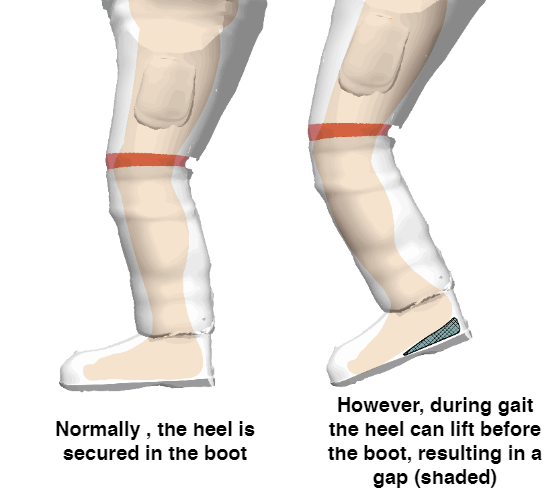
\includegraphics[width=0.6\textwidth,height=\textheight]{../fig/Background/HeelLift.png}
\caption{Heel-lift occurring during heel-off, as subjectively reported in the MK III. The poor fit and indexing in the boot and lower torso allows the heel to lift inside the boot during heel-off}\label{fig:B-HeelLift}
}
\end{figure}

\hypertarget{body-shape-characterization-to-improve-fit}{%
\subsection{Body Shape Characterization to Improve Fit}\label{body-shape-characterization-to-improve-fit}}

NASA's Anthropometry and Biomechanics Facility (ABF) has focused on characterizing the human body as it relates to spacesuit fit.
Linear measurements are traditionally used in sizing algorithms to determine a baseline suit fit.
These linear measurements are then compared to linear measurements in the suit's design to determine appropriate sizing components.
However, linear measurements do not always accurately represent a person's body shape \citep{Margerum2010}.
Three-dimensional scanning can help accurately characterize body-shape to allow for virtual fit testing against 3D models of the suit.
Boundary manikins can be generated which represent the extremities of accommodated anthropometry, and overlaid on 3D suit models to determine fit \citep{Margerum2010}.
Virtual fit check metrics may include penetration depth, contact areas, and overlap volume \citep{Kim2019}.
Monte-Carlo simulations of vast databases can also be virtually tested to find fit problems that may occur outside the boundary manikins \citep{Kim2019}.

However, static body shape may not be enough to ensure dynamic fit.
It is well known that parts of the body change shape during movement.
Capturing 3D-scans in multiple poses also allows for the development of a parametric models that can estimate how body shape changes with a specific movement; for example this can be used to check for shoulder clearance around the HUT \citep{Kim2016}.
This can greatly improve dynamic fit as it ensures the HUT accommodates the shoulder throughout its entire motion.
However, this methodology is limited to poses where the subject can pause between motions due to technological limitations for capturing dynamic body shape changes.

Body shape changes can also occur from exposure to an altered-gravity environment.
The ABF found on average posture to increase by a maximum of 3\%, hip circumference to decrease by a mean of 7\%, and thigh circumference to decrease by a mean of 10\% during microgravity spaceflight \citep{Kim2019}.
EMU sizing incorporates a 2.54cm increase in torso length to accommodate this change \citep{Thornton1987}.

Information from virtual fit testing can be incorporated into spacesuit design by informing where the internal geometry may need to be expanded or contracted to better fit the target population \citep{Kim2019}.
This process was used to validate the design of the Z2 suit.
However, it is virtually impossible to incorporate personal preferences of fit into this process; currently a threshold is implemented to determine acceptable levels of ease or compression \citep{Kim2019}.
In addition, modifying design to accommodate findings from fit can only be done to a certain extent; there are limitations on modifying the structure of an existing design while still meeting the same engineering requirements.
There are also no clear metrics for translating virtual fit testing into spacesuit component design, and current methodologies are limited to modifying the design of exisiting components rather than designing new components from the ground-up.

\hypertarget{summary-1}{%
\section{Summary}\label{summary-1}}

Ambulating on another surface and gravitational environment presents many challenges of its own, including changes in preferred gait patterns.
Wearing a stiff, pressurized spacesuit further increases the effort required to walk.
While constant volume joints may reduce pressurization effects, unquantified factors such as poor operator-spacesuit interaction may also be leading to injury.
Spacesuit fit is hard to characterize due to limited knowledge of in-suit motion and challenges including limited suit sizing components, limited suit design flexibility, an incomplete understanding of body shape changes, and lack of quantifiable metrics to validate fit.
Poor fit can reduce performance and lead to injury.
Ambulation specific fit issues, such as heel-lift, have been subjectively identified in the MK III but not fully quantified.
While there has not been a large scale study on injuries in the MK III, these fit issues are similat to the injury mechanisms leading to injury in the EMU.

Body-shape models have been proposed as a way to better fit operators to spacesuits.
Static body shape models allows for correctly sized spacesuit components to be selected and spacesuit component designs to be validated for accommodation of a target population.
Dynamic body shape models will ensure that dynamic fit is ensured throughout suit motions, but current technology is limited to capturing low-frequency motions.
In addition, there is no established framework for integrating dynamic body-shape models into the spacesuit design process.
Suit components designed around dynamic body shape models have not yet been tested for increased fit and comfort compared to traditionally designed and fitted suit components.

\hypertarget{investigative-rationale}{%
\chapter{Investigative Rationale}\label{investigative-rationale}}

The following gaps were identified from the previous research, as outlined in the literature review presented in the previous two chapters, and will motivate the direction of this thesis.

\begin{itemize}
\tightlist
\item
  \textbf{Gap 1: } Few efforts to quantify fit discrepancies

  \begin{itemize}
  \tightlist
  \item
    Subjective reports are currently used to identify fit discrepancies. While objective fit metrics can indicate decreased performance from poor fit, they cannot identify or confirm specific indexing discrepancies between the operator and spacesuit to support these specific reports.
  \end{itemize}
\item
  \textbf{Gap 2: } Limited knowledge on dynamic body shape changes due to motion

  \begin{itemize}
  \tightlist
  \item
    Current modeling of dynamic body shape relies on 3D capture of subjects pausing through the motion and interpolation of body shape between pauses. Technological challenges make it difficult to optically capture dynamic body shape changes where the subject cannot pause between the motion, such as during walking. Therefore, the lack of data makes it difficult to model these dynamic body shape changes.
  \end{itemize}
\item
  \textbf{Gap 3: } No existing framework for incorporating dynamic body-shape models into the spacesuit design and fit process

  \begin{itemize}
  \tightlist
  \item
    It is unclear how dynamic body shape models can be incorporated into both the design of spacesuit components, as well as used to virtually fit test proposed spacesuit components. Current efforts have proposed ways to modify currently designed spacesuit components, but not ways in which spacesuit components can be designed from scratch around dynamic body shape models.
  \end{itemize}
\item
  \textbf{Gap 4: } No studies to quantify the effect of using dynamic body-shape models over linear measurements on fit and mobility

  \begin{itemize}
  \tightlist
  \item
    Spacesuit components designed around body shape models have not been tested against traditionally design spacesuit components to show that they result in better fit and mobility.
  \end{itemize}
\end{itemize}

This proposed thesis will investigate the applicability of dynamic body shape models to improve fit and mobility for planetary EVA suit design.
To limit the scope of the work, the proposed work will focus on fit and mobility of the spacesuit boot.
The MK III spacesuit currently uses a pressurized modified hiking boot with a convoluted ankle joint and boot sizing inserts.
The boot is an important component for MK III ambulation and MK III boot fit has been identified as a key issue in suit fit, especially with the subjectively reported instances of heel-lift \citep{Fineman2018}.
While the thesis will focus on the foot-boot interface design, the novel contribution lies in the development of a experimental and design framework to translate body-shape changes into spacesuit design variables.
The proposed hypothesis of this work is therefore:

\begin{quote}
\textbf{Integrating dynamic body shape changes into the spacesuit boot design process will mitigate factors that lead to injury and improve compatibility between the operator and the spacesuit.}
\end{quote}

The proposed thesis will encompass the following specific aims:

\begin{itemize}
\tightlist
\item
  \textbf{Specific Aim 1: } Quantify instances of heel-lift in spacesuit gait

  \begin{itemize}
  \tightlist
  \item
    \emph{Motivation:} Heel-lift was subjectively reported as a potential symptom of poor fit during gait in the MK III, but was never quantified. Quantifying the level of heel-lift may lead to heel-lift can better inform boot design to mitigate this issue.
  \item
    \emph{Summary of Work:} Walking data was collected on the MK III by Fineman et al.~{[}2018{]}. This data was reanalyzed in the context of boot fit by analyzing vertical accelerations of the spacesuit's lower leg and operator's tibia. Heel-off times were detected using vertical accelerations. An analysis was conducted on quantifying displacement from vertical accelerations, but was found to have large margins of error. Therefore, this work proposes differences in heel-off times as an indicator of heel-lift and identifies a methodology directly quantify heel-lift in future work.
  \end{itemize}
\item
  \textbf{Specific Aim 2: } Predictively model dynamic changes in foot morphology during gait

  \begin{itemize}
  \tightlist
  \item
    \emph{Motivation:} The foot changes shape during the loading process of stance phase. Modeling these changes as they relate to subject anthropometry and kinematics will allow for prediction of dynamic foot shape during stance phase.
  \item
    \emph{Summary of Work:} A novel dynamic foot scanning system was developed to capture 4D foot scans from subjects walking on a treadmill. Dynamic foot scans were captured from thirty subjects as they walked on the treadmill. A predictive statistical shape model was developed to predict dynamic foot shape with an accuracy of 5.2 mm. From the model, the midfoot was found to decrease in girth as the foot is lifted through heel-off. Dynamic changes in the midfoot will be further studied across the population as it relates to instep height and instep girth.
  \end{itemize}
\item
  \textbf{Specific Aim 3: } Define and validate a design process integrating dynamic foot morphology data for a novel spacesuit boot

  \begin{itemize}
  \tightlist
  \item
    \emph{Motivation:} Existing knowledge on foot mobility can provide mobility requirements for a planetary spacesuit boot. Insight from the dynamic foot shape model can be integrated with these mobility requirements to develop a boot design that accommodates the mobility and dynamic shape of the boot.
  \item
    \emph{Summary of Work:} Mobility of the foot was characterized from the existing literature. A biomechanical design framework was developed to integrate these mobility requirements with the dynamic foot shape model developed in Specific Aim 2. This framework will be used to create a pressurized planetary spacesuit boot prototype.
  \end{itemize}
\item
  \textbf{Specific Aim 4: } Evaluate the prototype planetary spacesuit boot design for fit, comfort, and mobility

  \begin{itemize}
  \tightlist
  \item
    \emph{Motivation:} The planetary spacesuit boot design developed in Specific Aim 3 will be tested for improved fit and comfort as compared to a current MK III spacesuit boot design and a non-pressurized standard hiking boot. This will directly test the hypothesis of this thesis.
  \item
    \emph{Summary of Work:} The test subject will perform ROM tests in a glovebox with a vacuum, which will pressurize the boot. The subject will also perform heel lifts against a false floor simulate the heel-off phase of gait. Kinematics of the ankle and MTP joint will be captured. Methods from SA1 along with a contact sensor in the heel of the footwear will check for the heel-lift. Subjective surveys will assess the subject's fit and comfort levels. If the prototype boot design can achieve pressurization around the foot outside the glovebox, gait kinetics and kinematics will be captured with all three designs. The prototype boot may also be tested in conjunction with a full spacesuit, pending spacesuit testing availability.
  \end{itemize}
\end{itemize}

Analysis of heel-off times to indicate heel-lift has been completed in Specific Aim 1.
A dynamic foot scanning system was developed, and used to create a predictive dynamic foot shape model in Specific Aim 2.
This model is being used to study midfoot dynamic changes as they relate to population instep height and instep girth measurements.
The design framework has been defined in Specific Aim 3, and prototype boots are currently being iterated to validate the design framework.
Once the final prototype boots are constructed, they will be tested as described in Specific Aim 4.

\hypertarget{specific-aim-1-quantify-instances-of-heel-lift-in-spacesuit-gait}{%
\chapter{Specific Aim 1 : Quantify instances of heel-lift in spacesuit gait}\label{specific-aim-1-quantify-instances-of-heel-lift-in-spacesuit-gait}}

\hypertarget{introduction}{%
\section{Introduction}\label{introduction}}

Heel-lift is a subjectively reported fit issue in the MK III spacesuit, described as when the the operator's heel-lifts inside the boot before the boot's heel-lifts off the ground at heel-off \citep{Fineman2018}.
Heel-lift is an indicator of poor fit, leading to improper indexing of the ankle joint as the wearer goes to take a step.
This could lead to injury through excessive contact or ankle joint overuse when taking a step.
A better-fitting boot can help mitigate heel-lift by captures the heel to prevent it from lifting during heel-off.

Designing such a boot, however, is difficult without knowing the frequency and magnitude of heel-lift; the challenges of measuring in-suit motion means that no direct measurements have been taken to date.
Fineman et al. \citep{Fineman2018} used inertial measurement units (IMUs) to measure in-suit lower-torso kinematics of subjects walking with the MK III spacesuit.
IMUs measure the acceleration and orientation of the segment they're attached to, and have been successfully used in the biomechanics field to detect heel-off points during gait \citep{Rebula2013, Fischer2013}.
Heel-lift can be characterized as a lag between the operator's and spacesuit's heel-off times; essentially, the operator experiences heel-off prior to the spacesuit doing so.
IMUs were placed on both the operator's shank and the spacesuit's lower leg assembly (SLL), and it is assumed that the shank and SLL have a rigid connection their respective ankle joints.
Therefore, the difference between the shank's and SLL's vertical position taken after the operator's heel-off time is the magnitude of heel-lift.
While double-integrating an IMU's vertical acceleration signal is subject to integration drift, zero-velocity (ZVUs) and zero-position updates (ZPUs) have been used in the biomechanics field to correct for drift at every step \citep{Feliz2009, Rebula2013}.
However, IMUs are also subject to additional error in the spacesuit environment \citep{Bertrand2014, Shen2019, Shen2020}, bringing into question the feasibility of using these filtering methods on IMU data to detect heel-lift.

Therefore, this work aims to evaluate the ability of IMUs to quantify the frequency and magnitude of heel-lift through the following objectives:

\begin{itemize}
\tightlist
\item
  Detect heel-off times of both the spacesuit and the operator during suited walking trails where IMUs are placed on the lower-torso of both the spacesuit and operator
\item
  Evaluate the feasibility of zero-velocity and zero-position updates to reduce integration drift and quantify the magnitude of heel-lift
\end{itemize}

\hypertarget{methods}{%
\section{Methods}\label{methods}}

\hypertarget{experimental-design}{%
\subsection{Experimental Design}\label{experimental-design}}

Experimental data collected by Fineman et al. \citep{Fineman2018} was reanalyzed for this study.
Three subjects walked in the MK III spacesuit with different padding levels at the hip and knee.
Subject naming was kept consistent with Fineman et al. \citep{Fineman2018} for cross-reference of results, with subjects numbered 2-4 as Subject 1 did not complete all trials.
Padding is frequently used to help index the operator's joints to the spacesuit joints.
The subjects walked along a 10m walkway in each of four conditions: unsuited, MK III with no padding, MK III with one layer of padding, and MK III with two layers of padding.
Only the suited data was used in this analysis.
All three subjects wore the same size MK III lower-torso, but Subject 3 wore a BOA-laced boot while other subjects wore a standard strap-laced boot.
IMUs were placed in corresponding locations on the operator's and spacesuit's lower torso, while padding was placed in the pelvic and knee joints (fig.~\ref{fig:SA1-Loc}).

\begin{figure}
\hypertarget{fig:SA1-Loc}{%
\centering
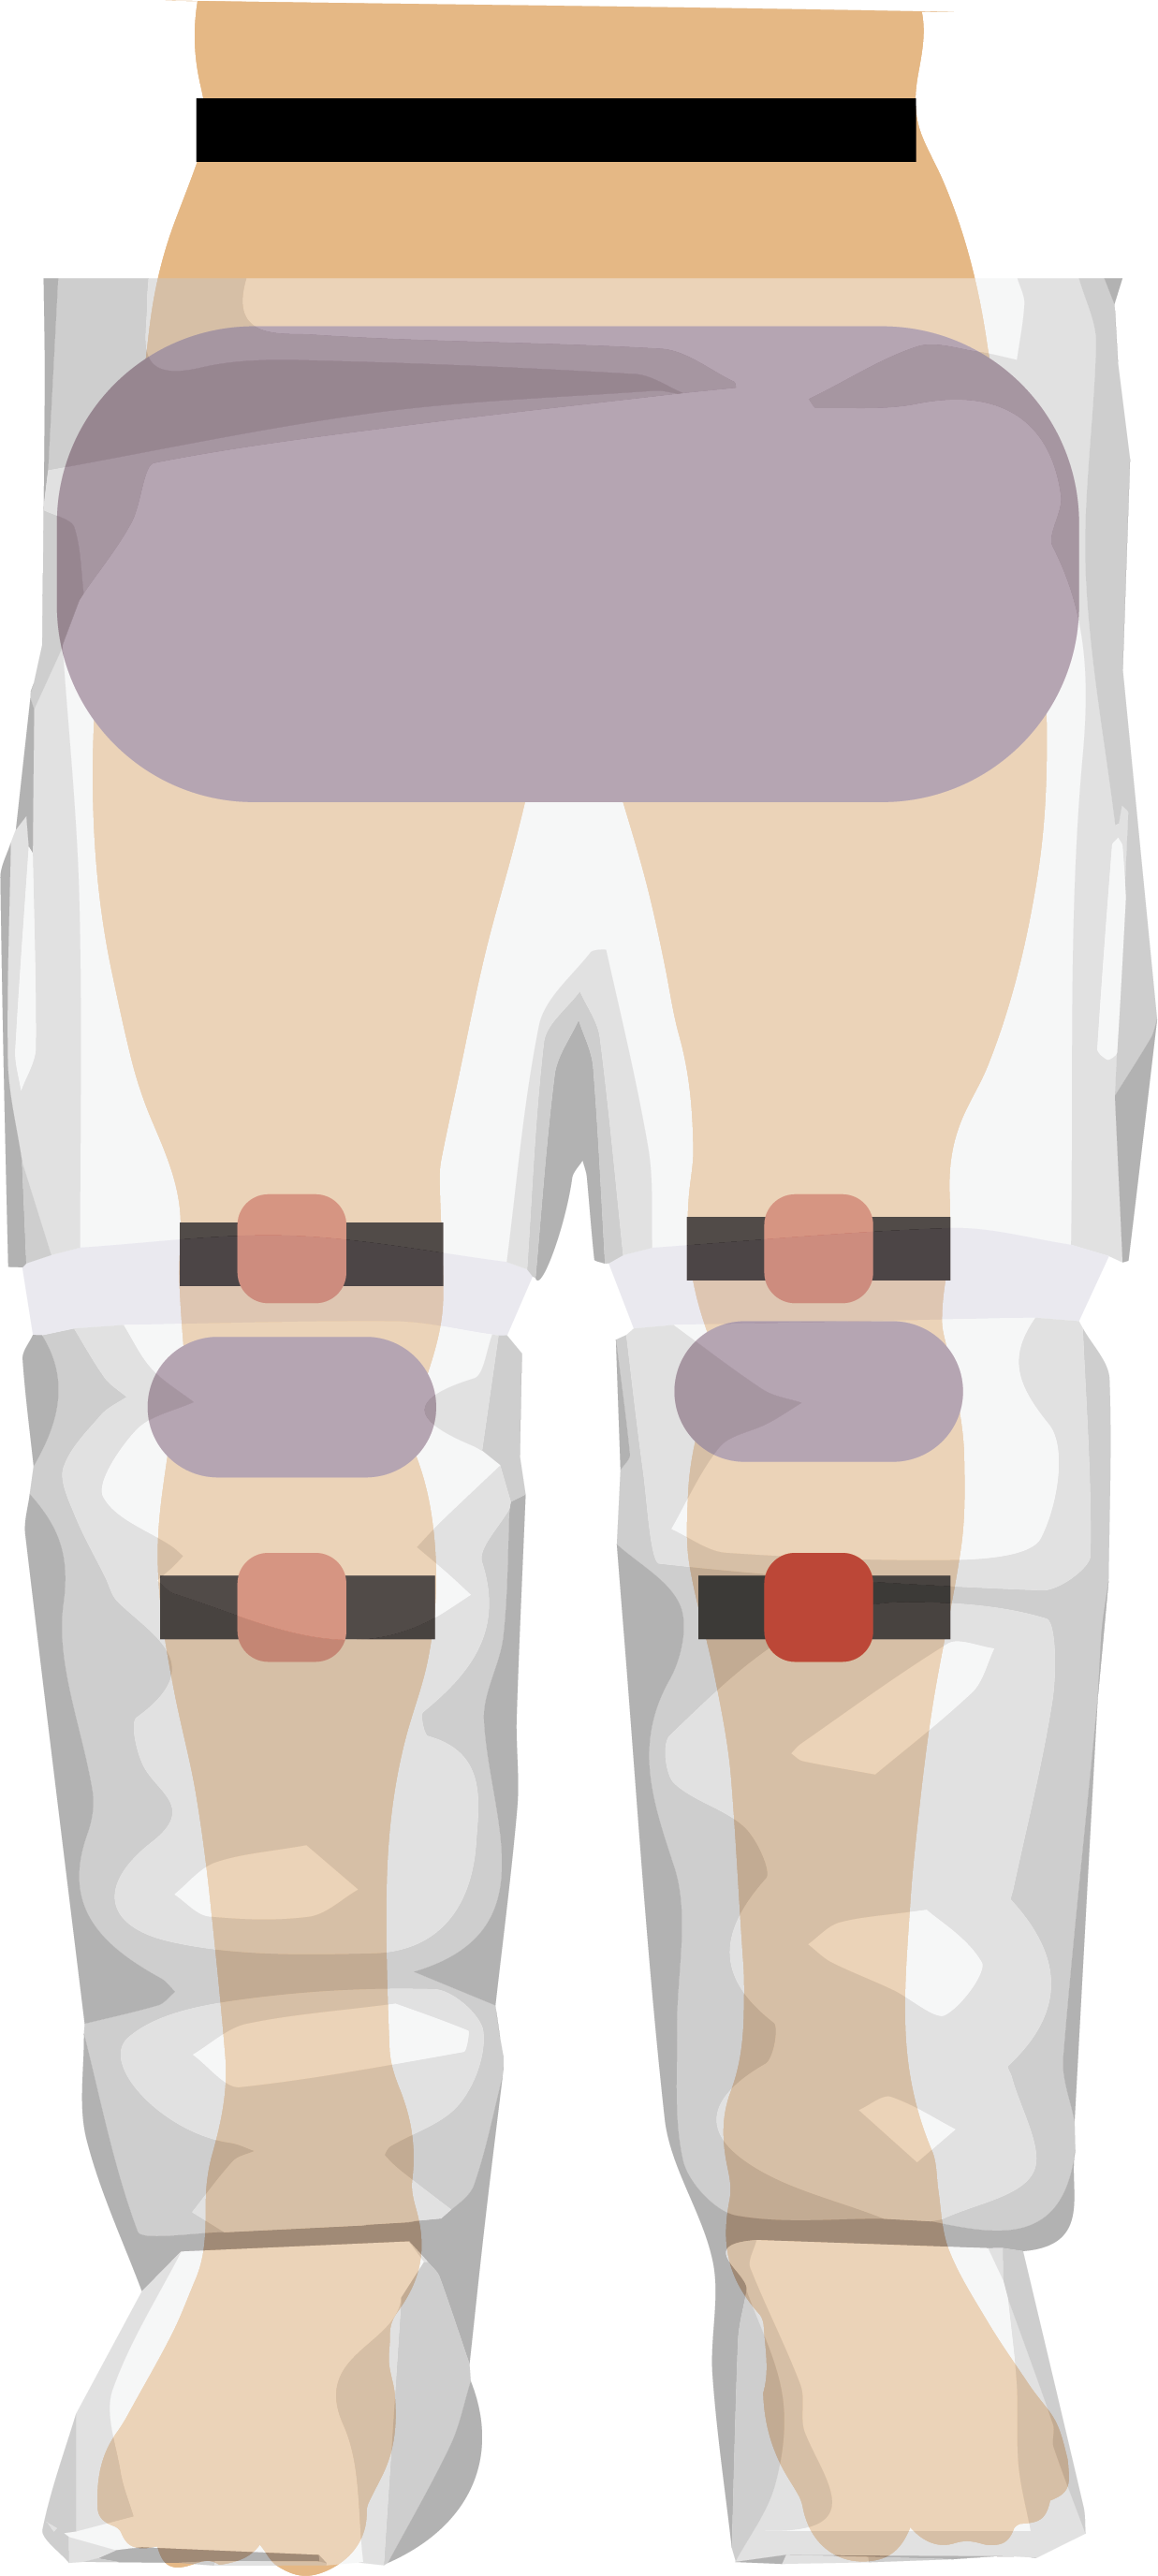
\includegraphics[width=0.7\textwidth,height=\textheight]{../fig/SA1/IMUPlacement.png}
\caption{Location of IMUs (red squares, placed both the spacesuit and operator) and padding (gray). The sacrum IMU is placed on the back of the operator and spacesuit, where the upper-most black band is located, and is therefore out of view in this diagram. The table on the right outlines the IMUs corresponding locations between the operator and spacesuit.}\label{fig:SA1-Loc}
}
\end{figure}

IMU vertical acceleration and pitch angle data from the operator's shank and the spacesuit's lower leg (SLL) was analyzed for this study.
A total of 216 trials were collected, each with data from the left and right sides of the operator and spacesuit, leaving 432 datasets to analyze.
For Subject 2, Configuration 2, the left shank IMU dropped out for 11 trials, leaving 421 total datasets.
For Subject 4, Configuration 0, Trials 1-12, the labels for the left and right IMUs seemed to be switched; the left SSL IMU was aligned with the right shank IMU and vice-versa.
Therefore, for these trials, the shank IMU was switched to the other side.
Since it isn't known which IMU in particular was mislabeled, it is unclear if the new labels are right for these trials.
However, since we are not analyzing our data by sides, this data was retained in the analysis.

\hypertarget{step-segmentation}{%
\subsection{Step Segmentation}\label{step-segmentation}}

Individual steps in the data for each trial was identified using detected peaks in the shank and SLL IMU's pitch angle.
These peaks are thought to correspond to the max posterior flexion/extension of the shank/SLL during the swing phase.
The pitch angle is first normalized to it's first value in the time series for each trial.
A moving average filter with a window of 10 samples, set through trial and error, was used to smooth the pitch angle.
The minimum peak distance is set to 1.5s to ensure high-frequency peaks are not detected; this parameter was set based on the observed length of each step typically taking longer than 1.5s.

Since the first and last peaks of the trail may not be complete steps, they were not included in the analysis.
Minimum peak prominence is set to 0.40 radians (23 degrees) to ensure that the first and last steps, which did not have complete swings, are not detected; peaks which corresponded to complete steps were observed to be closer to 0.60 radians (35 degrees).
Each step is defined as the time between each step's max extension to the following step's max extension.
An example of the step detection for a single trial is shown in fig.~\ref{fig:SA1-Steps}.

\begin{figure}
\hypertarget{fig:SA1-Steps}{%
\centering
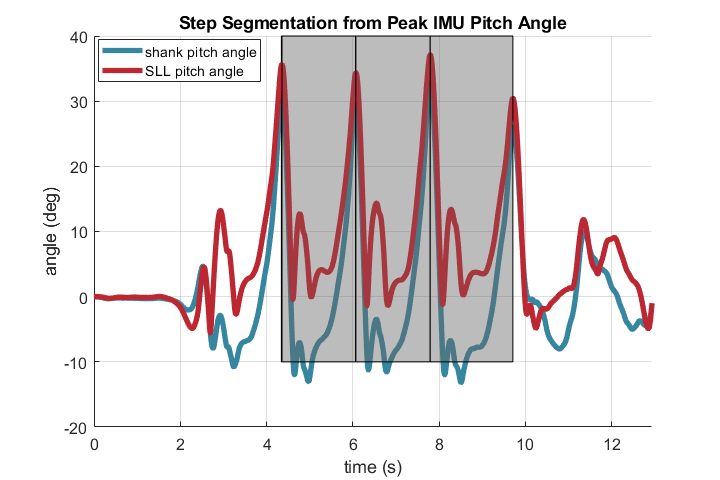
\includegraphics[width=0.7\textwidth,height=\textheight]{../fig/SA1/S3C1T1R_StepSeg.png}
\caption{Example of one dataset's step segmentation based on peak shank and SLL pitch angle. The shaded regions indicate discrete steps identified by the algorithm.}\label{fig:SA1-Steps}
}
\end{figure}

Once the locations of the peaks are detected, they are reshaped into an array which represents the start and end indices of each step.
Since the peak detection is not a perfect algorithm, the number of steps detected in one trial for the SLL and shank might not be the same.
Therefore, whichever IMU had the most amount of steps detected has its step times applied to the other IMU.
This only occurred in 57 out of the total 421 datasets, when a step may not meet the minimum peak prominence threshold for either the shank/SLL IMU while meeting the threshold for the other, leading it to not be counted.

\hypertarget{heel-off-timepoint-detection}{%
\subsection{Heel-Off Timepoint Detection}\label{heel-off-timepoint-detection}}

The foot-flat phase is the time duration within stance phase between toe-strike and heel-off, where the foot is flat on the ground; detecting foot-flat phase allows for the detection of the heel-off point.
This phase is characterized by very low anterior-posterior acceleration; since the foot is flat on the ground, there is very little vertical movement of the shank \citep{Rebula2013}.
Vertical acceleration data is preprocessed by first de-trending to remove bias by removing the best straight-fit line from the data vector.
A moving average filter with a window of 30 sample, equivalent to 0.23 seconds, is then used to remove noise, within the range used for walking-speed estimation \citep{Byun2019}.

Discrete wavelet transforms (DWT) can be used to detect gait events in from acceleration signals \citep{Ji2019}.
A 3-level discrete wavelet transform (DWT) is then applied to the preprocessed shank and SLL anterior-posterior acceleration signals.
A Symlets 2 wavelet (\texttt{sym2}) is used as the mother wavelet for the transform, due to its high performance in detecting initial-contact and final-contact points during stance phase \citep{Ji2019}.
After transforming to wavelet space, a threshold is applied where values below 2\% of the maximum wavelet coefficient are set to zero.
The wavelet coefficients are then reconstructed back into a signal and then used to detect foot-flat phase.

Foot-flat phase is detected by looking for the zero regions in the shank and SLL's acceleration's derivative \citep{Mariani2013}.
A threshold of \(0.01 m/s^{2}\) was set to account for small amounts of noise in the DWT signal.
Acceleration points within this threshold were identified as zero-acceleration points.
Zero-acceleration points less than 3-samples long are removed, since foot-flat phase is expected to be much longer.
The end of foot-flat phase is heel-off, while the beginning is toe-strike.
An example of detecting foot-flat phase is shown in fig.~\ref{fig:SA1-DWT}.
The difference in heel-off times between the shank and SLL can be used to detect instances of heel-lift; a positive value would mean the operator experience heel-off before the spacesuit, which would indicate heel-lift.
Quantifying these differences across all datasets can help determine the frequency of occurrence of heel-lift.

The heel-off detection was not perfect.
In some cases, it failed to properly detect heel-off for the operator or spacesuit with the parameters provided.
Heel-off lag times \textless-0.2s and \textgreater0.2s were manually inspected, and if the detection times were incorrect, these steps were taken out of the analysis.
Only 32 out of a total of 1381 steps met this criteria for removal.

\begin{figure}
\hypertarget{fig:SA1-DWT}{%
\centering
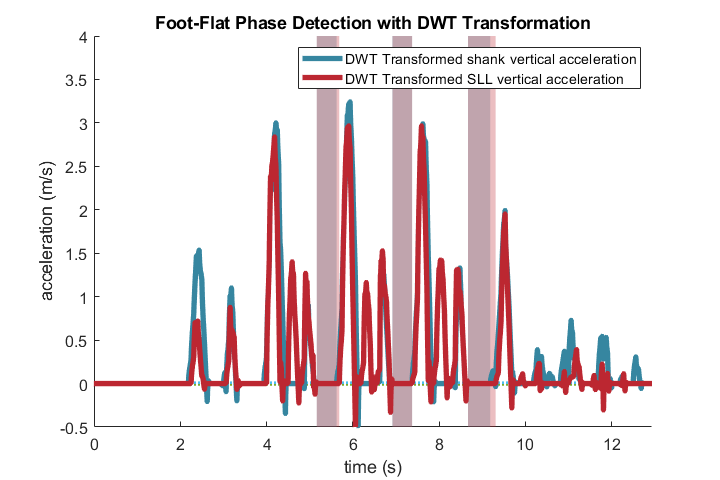
\includegraphics[width=0.7\textwidth,height=\textheight]{../fig/SA1/S3C1T1R_footflat.png}
\caption{Example of the foot-flat phase detection from the DWT thresholded vertical acceleration signal. The shaded regions represent detected foot-flat regions of zero-acceleration across the dataset.}\label{fig:SA1-DWT}
}
\end{figure}

\hypertarget{zero-velocity-zero-position-update}{%
\subsection{Zero Velocity / Zero Position Update}\label{zero-velocity-zero-position-update}}

Double-integrating the acceleration signal to calculate IMU position is subject to integration drift.
Zero-velocity (ZVU) and zero-position updates (ZPU) are used to reduce integration drift and improve the accuracy of the positional estimate of the shank and SLL.
The vertical acceleration signal is preprocessed by first detrending and then low-pass filtering at 10 Hz to remove high-frequency noise \citep{Antonsson1985}.
ZVUs rely on the fact that during gait, the vertical velocity of the shank or SLL will be zero during stance phase.
Therefore, this known fact can be used to correct the signal to zero during known stance phases.
At the identified heel-off times, the vertical velocity is set to 0, and the vertical velocity after heel-off is subtracted by the velocity reported at heel-off weighted based on the distance from the heel-off timepoint using formula eq.~\ref{eq:zvu}, originally presented by Feliz et al.~2009 \citep{Feliz2009}:
\begin{equation}\protect\hypertarget{eq:zvu}{}{
v'_{x,i} = v_{x,i} - v_{HO}*\frac{t_{i}-t_{TS}}{t_{HO}-t_{TS}}\\
}\label{eq:zvu}\end{equation}
where at timestep i after heel-off, \(v'_{x,i}\) is the corrected velocity, \(v_{x,i}\) is the original velocity, \(t\) is time, \(TS\) is the next toe strike timepoint, and \(HO\) is the next heel-off timepoint.
An example of how ZVUs reduce drift is shown in figure \ref{fig:drift}.
Integrating the corrected velocity signal to obtain the IMU's position will similarly be subject to integration drift.
It is assumed during stance phase that both the operator's foot and the spacesuit boot are flat on the ground and therefore the shank and SLL are not moving vertically.
ZPUs can use this known fact to correct for drift by zeroing the position estimate for both the SLL and shank at heel-off.
Since the shank and SLL are assumed to be rigidly connected to their respective ankle joints, taking the difference in shank and SLL vertical position after heel-off will give an estimate of heel-lift magnitude.

\begin{figure}
\hypertarget{fig:drift}{%
\centering
\includegraphics[width=0.7\textwidth,height=\textheight]{../fig/SA1/S3C1T1R_Drift.png}
\caption{Example showing how integration drift is reduced from de-trended and low-pass filtered vertical velocity signal (dotted lines) with ZVUs (solid lines), with vertical velocity now centered around zero}\label{fig:drift}
}
\end{figure}

\hypertarget{drift-rate-estimation}{%
\subsection{Drift Rate Estimation}\label{drift-rate-estimation}}

Since drift is not completely eliminated with the outlined methods, bounds need to be established where we can take the positional difference with confidence that the difference is not largely due to the drift.
While drift is not exactly a linear process, an assumption was made that calculating the drift magnitude between two known time points, and dividing it by the elapsed time, would be a reasonable approximation to quantify how drift accumulates over time in this scenario.
During stance phase, it's expected that both the SLL and shank will have the same vertical position at toe-strike and heel-off.
During swing phase, it is expected that both IMUs will return to the same vertical position after each step.
Drift magnitude was calculated for each detected step by subtracting the post-ZVU/ZPU position values at the beginning and end of stance phase and swing phase from each other, and then dividing by time of each phase, to get a drift rate.
This rate represents the amount the IMU's positional estimate has drifted over each phase following correction from ZVU/ZPUs, when it is expected to return to 0.
Analyzing the distribution drift rates across all trials will allow for a time-bound to be defined where drift magnitude is minimal and can ensure accuracy in the calculated position values.

\hypertarget{results}{%
\section{Results}\label{results}}

Median drift rates following ZVU/ZPUs for both the SLL and shank IMUs are presented in table \ref{tbl:SA1-drift}.
The SLL showed much higher drift rates than the shank, which may be due to that IMU being subject to the spacesuit's magnetic field disturbances.
The SLL drift rate during stance phase, where the heel-lift positional difference is taken following heel-off, therefore defines an upper confidence limit of 0.04 s to take a heel-lift measurement with an accuracy of 1 cm (1/26.33 cm/s).

\hypertarget{tbl:SA1-drift}{}
\begin{longtable}[]{@{}lll@{}}
\caption{\label{tbl:SA1-drift}Drift rate estimations of positional estimates for IMUs mounted on the spacesuit lower leg assembly and shank}\tabularnewline
\toprule
\begin{minipage}[b]{0.10\columnwidth}\raggedright
IMU\strut
\end{minipage} & \begin{minipage}[b]{0.41\columnwidth}\raggedright
Stance Phase Median Drift Rate\strut
\end{minipage} & \begin{minipage}[b]{0.41\columnwidth}\raggedright
Swing Phase Median Drift Rate\strut
\end{minipage}\tabularnewline
\midrule
\endfirsthead
\toprule
\begin{minipage}[b]{0.10\columnwidth}\raggedright
IMU\strut
\end{minipage} & \begin{minipage}[b]{0.41\columnwidth}\raggedright
Stance Phase Median Drift Rate\strut
\end{minipage} & \begin{minipage}[b]{0.41\columnwidth}\raggedright
Swing Phase Median Drift Rate\strut
\end{minipage}\tabularnewline
\midrule
\endhead
\begin{minipage}[t]{0.10\columnwidth}\raggedright
Shank\strut
\end{minipage} & \begin{minipage}[t]{0.41\columnwidth}\raggedright
9.48 cm/s\strut
\end{minipage} & \begin{minipage}[t]{0.41\columnwidth}\raggedright
14.15 cm/s\strut
\end{minipage}\tabularnewline
\begin{minipage}[t]{0.10\columnwidth}\raggedright
SLL\strut
\end{minipage} & \begin{minipage}[t]{0.41\columnwidth}\raggedright
26.33 cm/s\strut
\end{minipage} & \begin{minipage}[t]{0.41\columnwidth}\raggedright
27.48 cm/s\strut
\end{minipage}\tabularnewline
\bottomrule
\end{longtable}

Since 0.04 seconds is a very small amount of time in the context of gait events, it was decided to not record any heel-lift magnitudes as they would be much less than the 1 cm accuracy assumption used to derive the limit.
Measurements taken after this point may not be trustworthy due to the presence of accumulating drift.

Heel-off lag was calculated for all retained datasets.
Figure fig.~\ref{fig:heeloffdist} shows the distribution of heel-off lag measurements across all conditions and subjects.
Only Subject 4 experienced ``negative'' heel-off lag, where the spacesuit experiences heel-off before the operator. Subjects 2 and 3 experienced only ``positive'' heel-off lag, which would suggest that these subjects experienced heel-lift.
Example steps for these figures are shown in an example step is shown in fig.~\ref{fig:alllag}.

``Negative'' heel-off lag is theoretically impossible with the assumptions made in this study: when the spacesuit experiences heel-off, it will also push on the operator's heel, causing it to experience heel-off as well.
However, the assumption that the SLL is rigidly connected to the spacesuit's ankle was previously stated.
Since the SLL is made of soft goods, it can expand and contract in length due to internal pressure forces or interactions from the knee or femur.
Therefore, the SLL may be expanding in length for Subject 4 at heel-off, causing the IMU mounted on the SLL to register a positive acceleration and therefore the illusion that the spacesuit experiences heel-off before the operator.
This may not be concern for the shank-mounted IMU, as the shank is rigidly connected to the ankle and it is assumed that the IMUs are rigidly strapped to their segments.
It is also important to note that Subject 4 had larger lower-torso anthropometry than Subjects 2 or 3, which may cause greater leg lengthening.

\begin{figure}
\hypertarget{fig:heeloffdist}{%
\centering
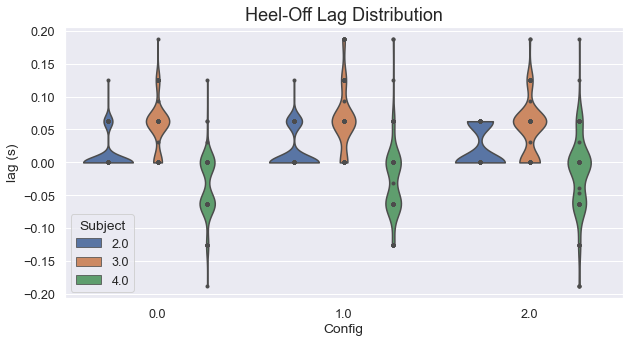
\includegraphics[width=0.7\textwidth,height=\textheight]{../fig/SA1/heelOffLag.png}
\caption{Heel-off lag distributions between all subjects and configurations, with discrete heel-off lag measurements being represented as black dots.}\label{fig:heeloffdist}
}
\end{figure}

\begin{figure}
\centering

\subfloat[A]{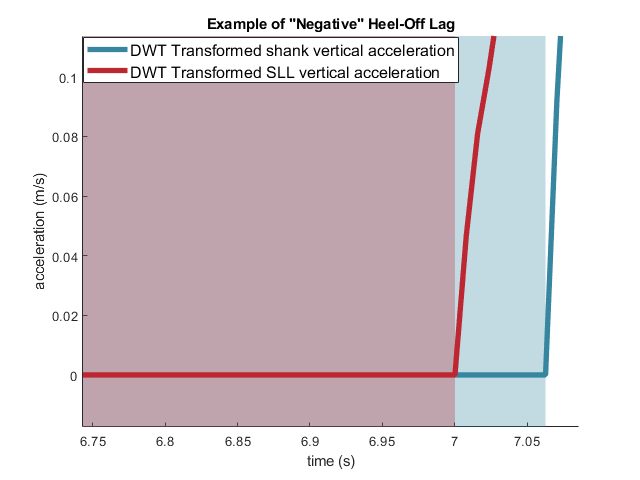
\includegraphics[width=0.5\textwidth,height=\textheight]{../fig/SA1/negHeelOff.png}\label{fig:alllagA}}\subfloat[B]{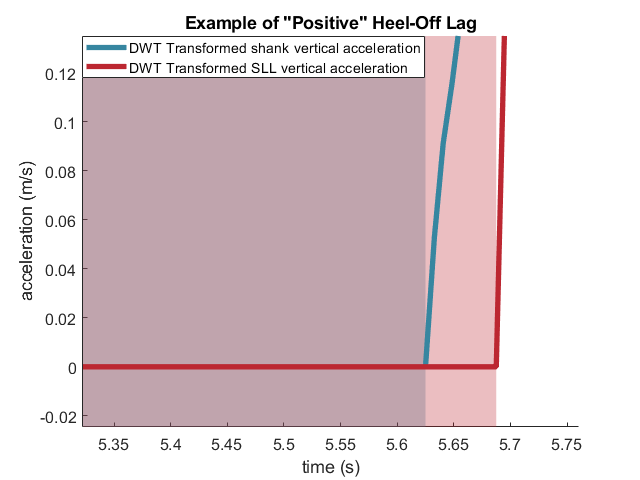
\includegraphics[width=0.5\textwidth,height=\textheight]{../fig/SA1/posHeelOff.png}\label{fig:alllagB}}

\caption{Zoomed-in view of one example step's foot-flat phase showing ``negative'' {[}A{]} and ``positive'' heel-off lag {[}B{]}. The shaded regions represent the detected foot-flat regions for the operator (blue) and spacesuit(red); an increase in vertical acceleration for the shank IMU (blue) prior to the SLL IMU (red) is ``positive'' heel-off lag, suggesting heel-lift {[}B{]}, and vice-versa {[}A{]}.}

\label{fig:alllag}

\end{figure}

\hypertarget{summary-2}{%
\section{Summary}\label{summary-2}}

The soft-goods design of the SLL does not allow for the accurate detection of heel-off lag between the shank and SLL since it breaks the assumption that the SLL is rigidly connected to the ankle.
In addition, ZVUs/ZPUs did not reduce integration drift enough to warrant using IMUs to measure heel-lift magnitude.

While the results of this study may not directly translatable to boot design, they do show that the SLL may be changing length during heel-off.
This can influence the forces acting on the boot, as well as the shank and knee of the operator.
Fineman et al \citep{Fineman2018} suggested that relative coordination of the lower-torso may be affected by boot fit issues, which may suggest that boot itself may be contributing to the forces extending the SLL.

Findings from this study suggest that current IMU technology may not be appropriate for quantifying the presence and magnitude of heel-lift in the spacesuit environment.
Future work may incorporate the use of contact sensors or pressure insoles in the spacesuit boot to check for heel-contact, along with optical capture of the spacesuit boot's kinematics to accurately detect heel-off points.
Such techniques can be used to augment the presented heel-off detection for the operator inside the spacesuit.
Improvements to IMU mounting on the spacesuit or characterization of the SLL leg lengthening may also decrease the effect of spacesuit pressure forces.
Updated sensor technology can also characterize the spacesuit leg lengthening effect, allowing it to be isolated from the IMU's signal.
Contact sensors and pressure insoles will be evaluated for testing in Specific Aim 4.

Currently, all analysis is complete with this work.
This work is currently in preparation as a technical note to be submitted for peer-review.

\hypertarget{specific-aim-2-predictively-model-dynamic-changes-in-foot-morphology-during-gait}{%
\chapter{Specific Aim 2: Predictively model dynamic changes in foot morphology during gait}\label{specific-aim-2-predictively-model-dynamic-changes-in-foot-morphology-during-gait}}

\hypertarget{introduction-1}{%
\section{Introduction}\label{introduction-1}}

Designing a new spacesuit boot to be more comfortable and not be subject to fit issues like heel-lift, requires a thorough understanding of foot shape.
However, foot shape is known to be highly variable throughout the population, including by sex \citep{Wunderlich2001, Krauss2008, Krauss2010}, age \citep{Tomassoni2014}, and weight \citep{Price2016}.
This variability is often not captured in terrestrial footwear sizing, as current fitting standards only use foot length, foot width, and arch length to fit to standardized shoe sizes \citep{ASTM2017}.
Furthermore, terrestrial footwear is commonly designed around lasts, shoe molds that are sized and shaped by each manufacturer with no common standard.
This leads to variability in footwear shapes and sizes \citep{Jurca2013, Wannop2019}, making it hard for consumers to find a proper fit and resulting in users having to wear ill-fitting footwear with suboptimal comfort.
Foot problems and resultant pain have been reported due to poor fit in coal mining boots \citep{Dobson2018b}.
Therefore, the issue of footwear fit is not just limited to spacesuit boots, both terrestrial footwear and spacesuit boots should account for the wide variety of foot shapes to improve fit.

In addition to foot shape variability in the population, the foot also changes shape while being loaded during gait.
The current methodology of designing terrestrial footwear uses static lasts, assuming that the foot consists of rigid segments.
Assumptions of rigid foot segments during foot loading have shown inaccuracies in estimation of ankle joint mechanics \citep{Zelik2018, Kessler2020}, suggesting intra-foot motion as the foot is loaded \citep{Lundgren2008, Wolf2008}.
Evidence suggests that foot loading affects linear foot measurements, such as when transitioning from sitting to standing \citep{Xiong2009, Oladipo2008} or during the stance phase of gait \citep{Kouchi2009, Barisch-Fritz2014, Grau2018}.
The dynamically changing measurements suggest morphological changes occurring, all of which may not be captured in static linear and circumferential measurements.
Thus, footwear should also be designed to account for these dynamic foot shape changes.

Statistical shape models (SSMs) can explain morphological differences across populations and during motion by identifying shape modes which account for variance from the mean shape.
These have been developed for whole-body digital human modeling applications to study population and individual variance in body shape \citep{Allen2003, Anguelov2005, Reed2014, Park2015a, Park2017}.
Parametric SSMs are extensions which use correlations between subject anthropometric data and SSM deformations to help predict body shape for new individuals in the population \citep{Park2015a, Park2017}.
The ABF at NASA developed parametric SSMs to characterize shoulder shape deformation across the shoulder's range-of-motion, predicting shape as a function of shoulder orientation, to validate HUT design \citep{Kim2016, Kim2019}.
However, the technology used to capture the body scans for this SSM could not capture the dynamic natural motion of the shoulder; subjects had to pose their shoulder at specific orientations while a scan was taken.

SSMs have recently been applied to characterize static foot shape across a population \citep{Conrad2019} and recognize foot-shape deviations \citep{Stankovic2020}.
The aforementioned efforts to capture foot measurement changes over the gait cycle did capture 4D foot images at high framerates \citep{Barisch-Fritz2014, Grau2018}, but these efforts were not translated into a SSM.
Previously developed systems were based on a catwalk, requiring subjects to correctly hit the scanning area for a successful data capture, which may not be representative of natural cadence.
However, the systems used to capture 4D foot shape are very expensive and cannot be used around a treadmill, which allows for subjects to fall into natural gait.
No SSMs have been developed from previous capture of 4D foot scans to predict dynamic foot shape

Therefore, the objectives of this specific aim are:

\begin{itemize}
\tightlist
\item
  Develop a low-cost 4D scanning system capable of capturing foot shape around a treadmill
\item
  Create a predictive model of foot shape changes across the dorsal surface during stance phase
\item
  Identify specific areas of the foot that change shape during stance phase
\item
  Correlate changes in foot shape across large-scale population foot measurements
\end{itemize}

\hypertarget{dynamo-dynamic-body-shape-capture-with-intel-realsense-cameras}{%
\section{DynaMo: Dynamic Body Shape Capture with Intel RealSense Cameras}\label{dynamo-dynamic-body-shape-capture-with-intel-realsense-cameras}}

A low-cost 4D scanning system, DynaMo, was developed to capture dynamic foot shape during gait.
Human body shape can be captured with a variety of methodologies, including laser lines, structured light, photogrammetry, and millimeter waves \citep{Daanen2013}.
However, these technologies require expensive modules and have limited ability to capture dynamic changes in body shape.
Motion capture with specific markers is commonly done through camera-based motion tracking \citep{Windolf2008}
These systems for marker tracking are often cost prohibitive and unable to capture surface morphology.

Therefore, the DynaMo software library was developed to use multiple commercial depth cameras, the Intel RealSense DXX Depth Cameras (Intel, Santa Clara CA), retailing between \$150-\$200, to capture dynamic body shape changes.
The Intel RealSense Depth cameras use two stereo image sensors along with a structured light projector to capture depth maps at 90 frames-per-second; each pixel in a depth map records the distance from the camera to the world.
DynaMo includes functions to calibrate a capture volume, using a checkerboard to identify a common origin between multiple depth cameras (fig.~\ref{fig:testSetup}).
DynaMo calculates a common point cloud from the depth maps of all the connected cameras, outputting a point cloud for every frame captured by all connected cameras (fig.~\ref{fig:SA2-sampleFrames}).
Functions were also developed to track the position of reflective markers in the scene.
The development of DynaMo was published in a journal paper \citep{Boppana2019}.

\begin{figure}
\hypertarget{fig:testSetup}{%
\centering
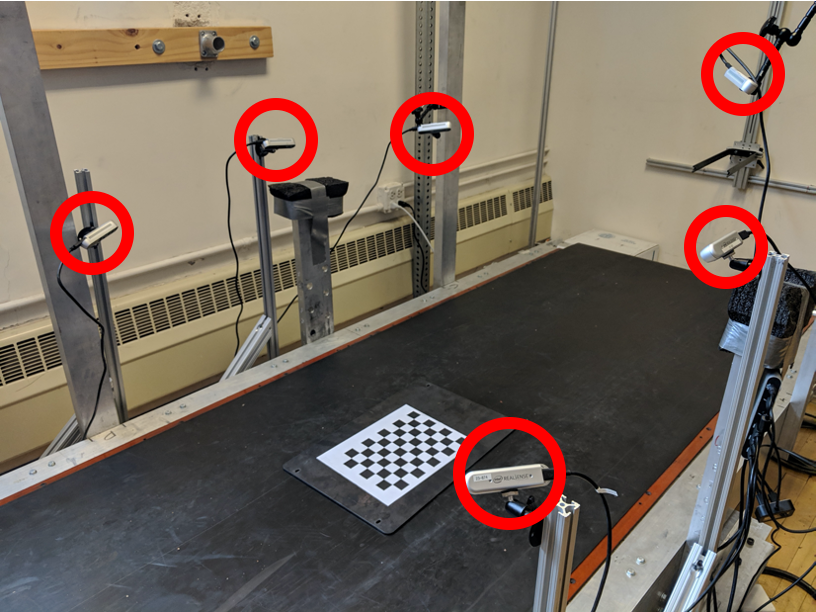
\includegraphics[width=0.5\textwidth,height=\textheight]{../fig/SA2/capturesetup.png}
\caption{Capture setup of 6 Intel RealSense D415 Depth Cameras (circled in red) placed around a treadmill. The checkerboard shown was used to calibrate the cameras using the DynaMo package.}\label{fig:testSetup}
}
\end{figure}

\begin{figure}
\hypertarget{fig:SA2-sampleFrames}{%
\centering
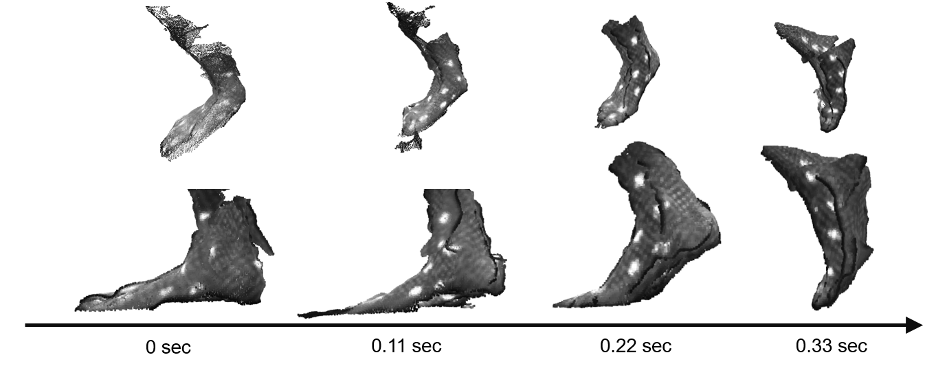
\includegraphics[width=0.8\textwidth,height=\textheight]{../fig/SA2/sampleFrames.png}
\caption{Sample frames, shown in 10 frame intervals (bottom), collected by DynaMo showing dynamic shape capture of the foot (top) at 90 frames-per-second, and the capture of reflective markers on the foot shown as white dots}\label{fig:SA2-sampleFrames}
}
\end{figure}

\hypertarget{development-of-a-predictive-dynamic-foot-shape-model-from-statistical-shape-modeling}{%
\section{Development of a Predictive Dynamic Foot Shape Model from Statistical Shape Modeling}\label{development-of-a-predictive-dynamic-foot-shape-model-from-statistical-shape-modeling}}

The development of the DynaMo software \citep{Boppana2019} allowed for a capturing of foot shape to develop a parametric SSM.
This system captures foot morphology changes during loading and unloading on the foot's dorsal surface, but does not capture of the foot's plantar surface.
A parametric SSM was developed which can characterize and predict dynamic foot morphology at specific points during stance phase across the subject population.

\hypertarget{methods-1}{%
\subsection{Methods}\label{methods-1}}

\hypertarget{subjects}{%
\subsubsection{Subjects}\label{subjects}}

A total of 30 healthy subjects (15 men and 15 women, ages 23.1 \(\pm\) 3.7) participated in this study.
Subjects were recruited in a stratified sample into one of six groups (5 subjects per group) to maximize variance in population foot length.
Height was used as the grouping factor since height is well correlated to foot length \citep{Giles1991}. The general population may not know offhand their exact foot length, and shoe size varies by manufacturer and does not correspond directly to foot length \citep{Jurca2013, Wannop2019}. Groups consisted of 5th-35th, 35th-65th, and 65th-95th height percentiles for each sex.
Height percentile values were taken from the ANSUR II survey \citep{Gordon2014} and converted to imperial units as it was expected most subjects would report their height in imperial units.
Population recruitment groups are summarized in tbl.~\ref{tbl:groups}.

\hypertarget{tbl:groups}{}
\begin{longtable}[]{@{}llll@{}}
\caption{\label{tbl:groups}Enrollment groups based on reported height. 5 subjects were enrolled in each group}\tabularnewline
\toprule
\begin{minipage}[b]{0.13\columnwidth}\raggedright
Sex\strut
\end{minipage} & \begin{minipage}[b]{0.25\columnwidth}\raggedright
5th-35th percentile Height\strut
\end{minipage} & \begin{minipage}[b]{0.25\columnwidth}\raggedright
35th-65th percentile Height\strut
\end{minipage} & \begin{minipage}[b]{0.25\columnwidth}\raggedright
65th-95th percentile Height\strut
\end{minipage}\tabularnewline
\midrule
\endfirsthead
\toprule
\begin{minipage}[b]{0.13\columnwidth}\raggedright
Sex\strut
\end{minipage} & \begin{minipage}[b]{0.25\columnwidth}\raggedright
5th-35th percentile Height\strut
\end{minipage} & \begin{minipage}[b]{0.25\columnwidth}\raggedright
35th-65th percentile Height\strut
\end{minipage} & \begin{minipage}[b]{0.25\columnwidth}\raggedright
65th-95th percentile Height\strut
\end{minipage}\tabularnewline
\midrule
\endhead
\begin{minipage}[t]{0.13\columnwidth}\raggedright
Female\strut
\end{minipage} & \begin{minipage}[t]{0.25\columnwidth}\raggedright
4'11``-5'3''\strut
\end{minipage} & \begin{minipage}[t]{0.25\columnwidth}\raggedright
5'3``-5'5''\strut
\end{minipage} & \begin{minipage}[t]{0.25\columnwidth}\raggedright
5'5``-5'8''\strut
\end{minipage}\tabularnewline
\begin{minipage}[t]{0.13\columnwidth}\raggedright
Male\strut
\end{minipage} & \begin{minipage}[t]{0.25\columnwidth}\raggedright
5'4``-5'8''\strut
\end{minipage} & \begin{minipage}[t]{0.25\columnwidth}\raggedright
5'8``-5'11''\strut
\end{minipage} & \begin{minipage}[t]{0.25\columnwidth}\raggedright
5'11``-6'2''\strut
\end{minipage}\tabularnewline
\bottomrule
\end{longtable}

Prior to recruitment, subjects completed a prescreening survey to ensure they were adequately healthy by the American College of Sports Medicine guidelines \citep{Riebe2015}, and between the ages of 18-65.
Subjects provided their sex and height, and were only enrolled in the study if their population group was not fully enrolled.

\hypertarget{experimental-procedures}{%
\subsubsection{Experimental Procedures}\label{experimental-procedures}}

The experimental protocol was approved by the University of Colorado Institutional Review Board.
Procedures were explained to each subject and written consent was obtained prior to participation.
Subjects' height and weight were recorded with a tape measure and scale, respectively.
Subjects' foot length, foot width, and arch length were measured with a Brannock device (The Brannock Device Company, Liverpool, NY) \citep{ASTM2017}.
Both foot length and arch length were measured in centimeters.
Foot width was measured as an ordinal size (e.g.~A, B, C, D, E), and then converted to a linear measurement in centimeters (The Brannock Device Company, Liverpool, NY).

Six Intel RealSense D415 Depth Cameras (Intel, Santa Clara, CA) were placed and calibrated around a custom-built level treadmill in the University of Colorado Boulder Locomotion Laboratory, as shown in fig.~\ref{fig:testSetup}.
The treadmill was set to an average walking pace of 1.4 m/s \citep{Browning2006}.
Reflective markers were placed on the subject's right foot and a black sock over their left foot to aid in right foot identification.
Subjects first walked for one minute to warm-up and fall into a natural cadence.
The operator then collected 10 seconds of data to capture approximately 10 steps.
The data were reviewed to ensure the subject stayed in frame from heel-strike to toe-off during capture. If needed, the subject's placement was shifted and data was collected again, up to two times.

\hypertarget{data-processing}{%
\subsubsection{Data Processing}\label{data-processing}}

Figure \ref{fig:dataflow} provides an overview of the data processing workflow; all steps are summarized in the paragraphs below.

\begin{figure}
\hypertarget{fig:dataflow}{%
\centering
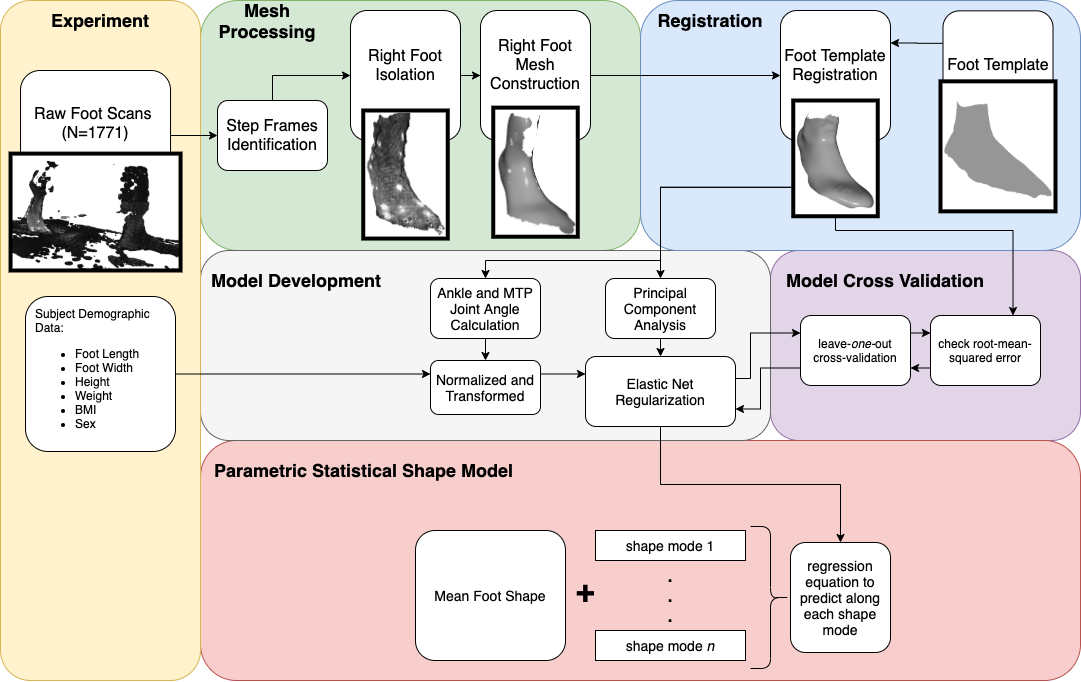
\includegraphics[width=1\textwidth,height=\textheight]{../fig/SA2/footProcessing.png}
\caption{Flowchart of processing steps for statistical shape model creation}\label{fig:dataflow}
}
\end{figure}

For each subject, a candidate heel-strike to toe-off event was manually identified across all captures by taking into account point cloud quality due to the high computational power required to process all heel-strike to toe-off events.
The depth images captured by each depth camera were processed into point clouds using the DynaMo package \citep{Boppana2019}.
From each point cloud, the right foot was isolated and transformed into a triangle mesh \citep{Rusu2011, Fischler1981, Bernardini1999, Zhou2018}.
Since every depth image was captured independently by the cameras, the amount and location of points which represented the foot were not consistent.
In addition, the captured data may have holes in the surface representing the foot.
Registration of all scans to a common template represents every scan by an equal number of points, and ensures any missing points are properly interpolated.
The right foot meshes were then iteratively registered using a three-step fitting process to an averaged high-quality static template scan, provided by Dr.~Matthew Reed from the University of Michigan Transportation Research Institute \citep{Reed2013}.
First scans were roughly aligned using a point-to-plane iterative-closest-point algorithm \citep{Chen1992}, implemented in Open3D \citep{Zhou2018}.
Next, the radial-basis function fitting algorithm from the GIAS2 software package \citep{Zhang2016} was run twice using a thin-plate spline to approximate the foot surface \citep{Park2015a, Kim2016}.
The mid-stance scan from each subject was registered first to the template, and then the registration process was run both forwards towards toe-off and backwards towards heel-strike, on a scan-by-scan basis, using the previously registered scan as a template for the next scan.
Accuracy was checked by comparing registered scans with the processed scans by finding corresponding points between both, and calculating the root-mean-squared error (RMSE) between the corresponding points.

Anatomical landmarks can be reliably approximated from the registered scans \citep{VandenHerrewegen2014b}.
The first metatarsal head, fifth metatarsal head, and second toe landmarks were used to align all scans to be centered at the second metatarsal head, with the forward axis pointing towards the second toe.
Landmarks around the metatarsal-phalangeal (MTP) joint and ankle joint were used to calculate ankle, MTP, and foot kinematics for each subject's scans with respect to the joint angles at the subject's mid-stance scan.
Relevant joint angles include dorsi/plantarflexion, ankle inversion/eversion, ankle internal/external rotation, MTP dorsi/plantarflexion, foot inversion/eversion, and foot internal/external rotation angles.

\hypertarget{model-construction}{%
\subsubsection{Model Construction}\label{model-construction}}

Principal component (PC) analysis is a dimensionality-reduction method commonly in constructing SSMs \citep{Reed2008, Park2015a, Conrad2019, Stankovic2020}.
The first PC represents an axis containing the largest variance in the dataset, and each subsequent PC describes the largest variance orthogonal to the previous component's axis.
Therefore, PCs allow for a new, smaller set of orthogonal variables to be defined which represent the variance in the dataset.

Let \(N\) equal the number of total scans in the dataset, and \(n=29873\) equal the number of vertices in each registered scan. The scikit-learn module \citep{JMLR:v12:pedregosa11a} was used to incrementally calculate the maximum \(N\) PCs which represent the dataset.
Each scan in the dataset is represented in the PC model with \(N\) PC scores.
All PC scores are centered around 0, which represents the mean foot scan of the dataset containing all subjects.
Each PC represents a shape mode in the SSM, where each score represents a deviation from the mean foot along the shape mode axis. The resultant PC model can be used to inverse transform a vector of length \(N\) PC scores into a \(29873\times 3\) vector, which represents the location of the vertices in the foot shape. Not all PCs were retained in the model since the first few PCs explain a majority of the variance, while additional PCs may be accounting for noise.

Subject demographic data and calculated joint angles were incorporated into the SSM by developing multivariate linear regression models based on these features.
This was used to predict each PC score, which can then be inverse-transformed into a foot shape.
Subject demographic data and joint angles were normalized and power-transformed to aid in regression development \citep{Yeo2000}.
An elastic net regularization algorithm \citep{Zou2005} was run for each multivariate regression to calculate normalized feature coefficients for each PC score's regression.
Two different sets of predictors were created, one with all subject demographic data and calculated joint angles, and one with the highly cross-correlated predictors of arch length, body-mass index, and height were removed.
Six potential models were built as combinations between the number of PCs predicted which explained 95\%, 98\%, and 99.7\% of the variance, and the two predictor sets.

\hypertarget{model-validation}{%
\subsubsection{Model Validation}\label{model-validation}}

All six models were validated for performance using leave-one-out cross-validation, where scans from each subject were set as the validation set, and models were trained on the remaining dataset.
Model performance during validation was quantified with the root mean squared error (RMSE) of the predicted foot shape to the corresponding registered scan.
A two-way RMANOVA analysis was run on the error distributions to test the effect of constructing a predictor with the different number of PCs, and between using the two variable sets.
The chosen model was retrained on the whole dataset before being analyzed.

\hypertarget{results-1}{%
\subsection{Results}\label{results-1}}

A total of 1771 scans were analyzed across all 30 subjects.
The average number of scans collected for each subject's stance phase was 59 \(\pm\) 3.7, with a range of 52-69 scans due to inter-individual differences in stride length.
Figure \ref{fig:scans} shows a set of raw and registered scans from one subject.
All processed scans were registered to the template with a median registration accuracy of 1.0 \(\pm\) 0.6 mm.

\begin{figure}
\hypertarget{fig:scans}{%
\centering
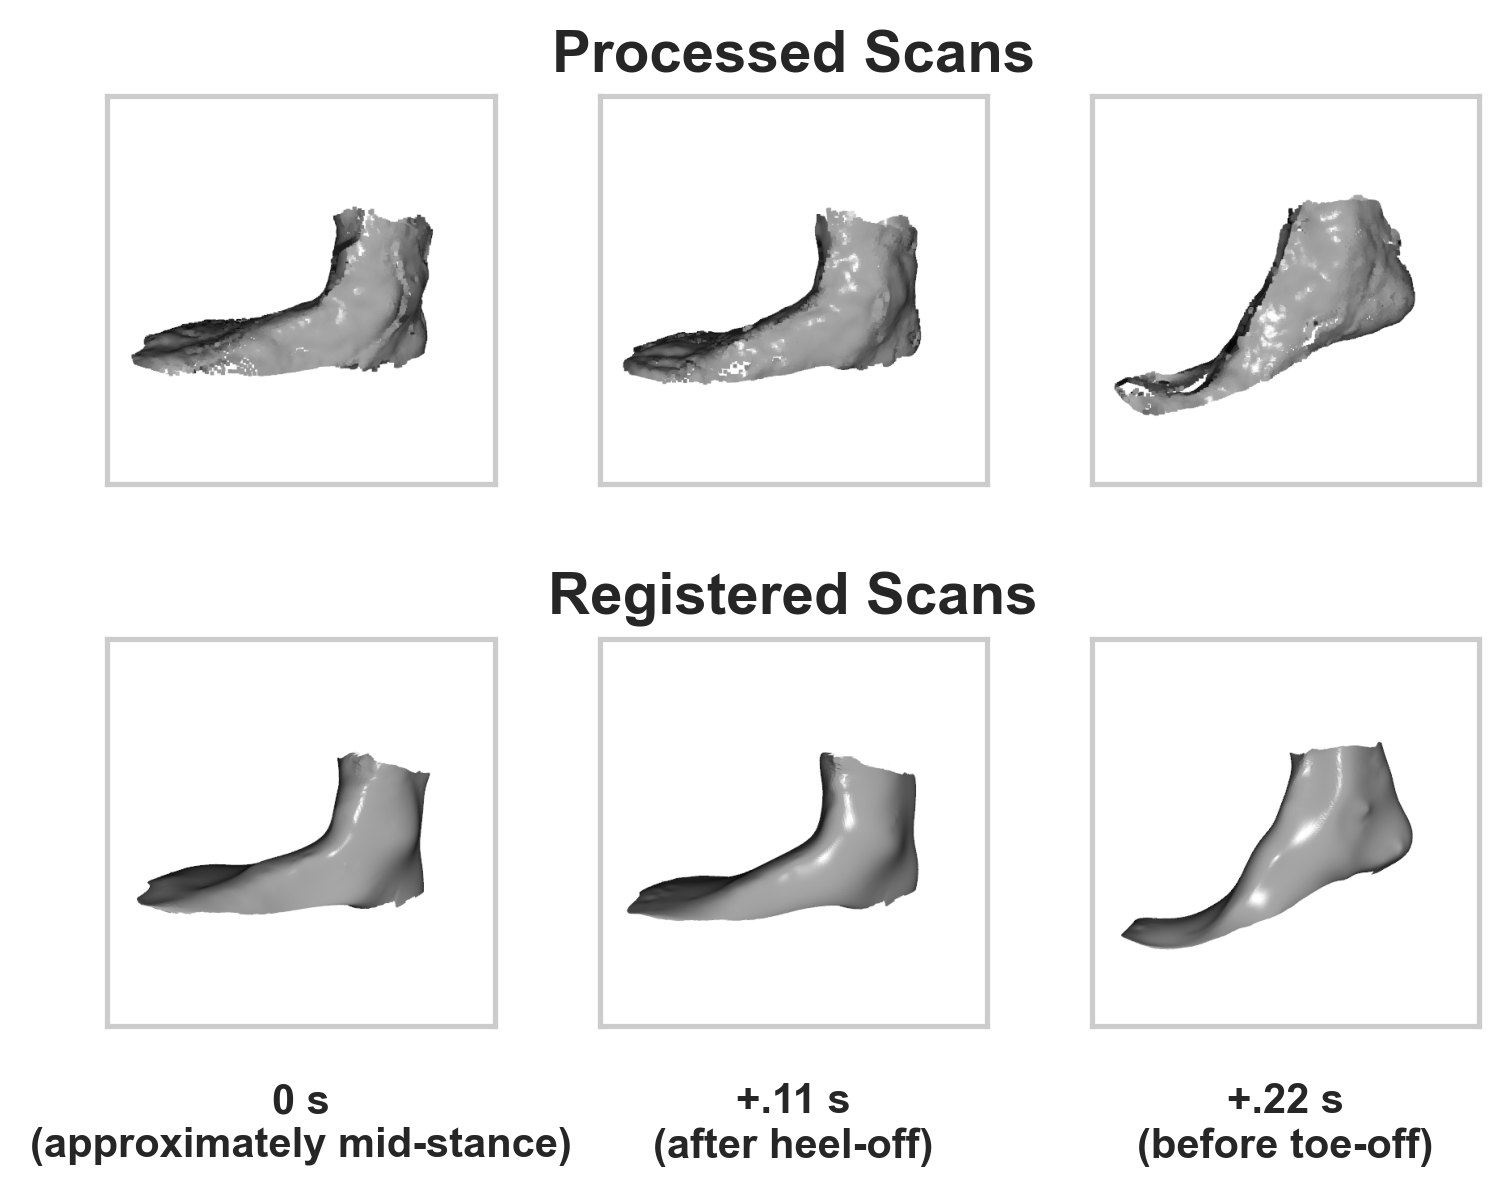
\includegraphics[width=0.8\textwidth,height=\textheight]{../fig/SA2/scans.png}
\caption{Processed and registered scans of one subject during heel-off, shown 10 frames (0.11 seconds) apart.}\label{fig:scans}
}
\end{figure}

The PCA analysis of all registered scans found the first 8 PCs to represent approximately 95\% of the variance, the first 27 PCs to represent approximately 98\% of the variance, and the first 105 PCs to represent approximately 99.7\% of the variance.
Figure \ref{fig:modelperf} shows the distribution of cross-validation RMSEs for each of the six elastic net regression models tested.
RMSE distributions did not meet assumptions for normality, but RMANOVA was still used to compare models due to its resiliency to deviations from normality.
A significant difference was found between predicting different numbers of PCs (F=1595.0, p\textless0.001), predicting between the two variable sets (F=81.6, p\textless0.001), and the interaction between both factors (F=213.7, p\textless0.001).
Significant differences were found between all three levels of the predicted number of PCs (p-adj\textless0.001) with a Tukey post-hoc HSD test.
No significant difference was found between the two variable sets (p-adj=0.42).
Therefore, the model predicting 8 PCs with the selected variable set was chosen for its simplicity and performance.

\begin{figure}
\hypertarget{fig:modelperf}{%
\centering
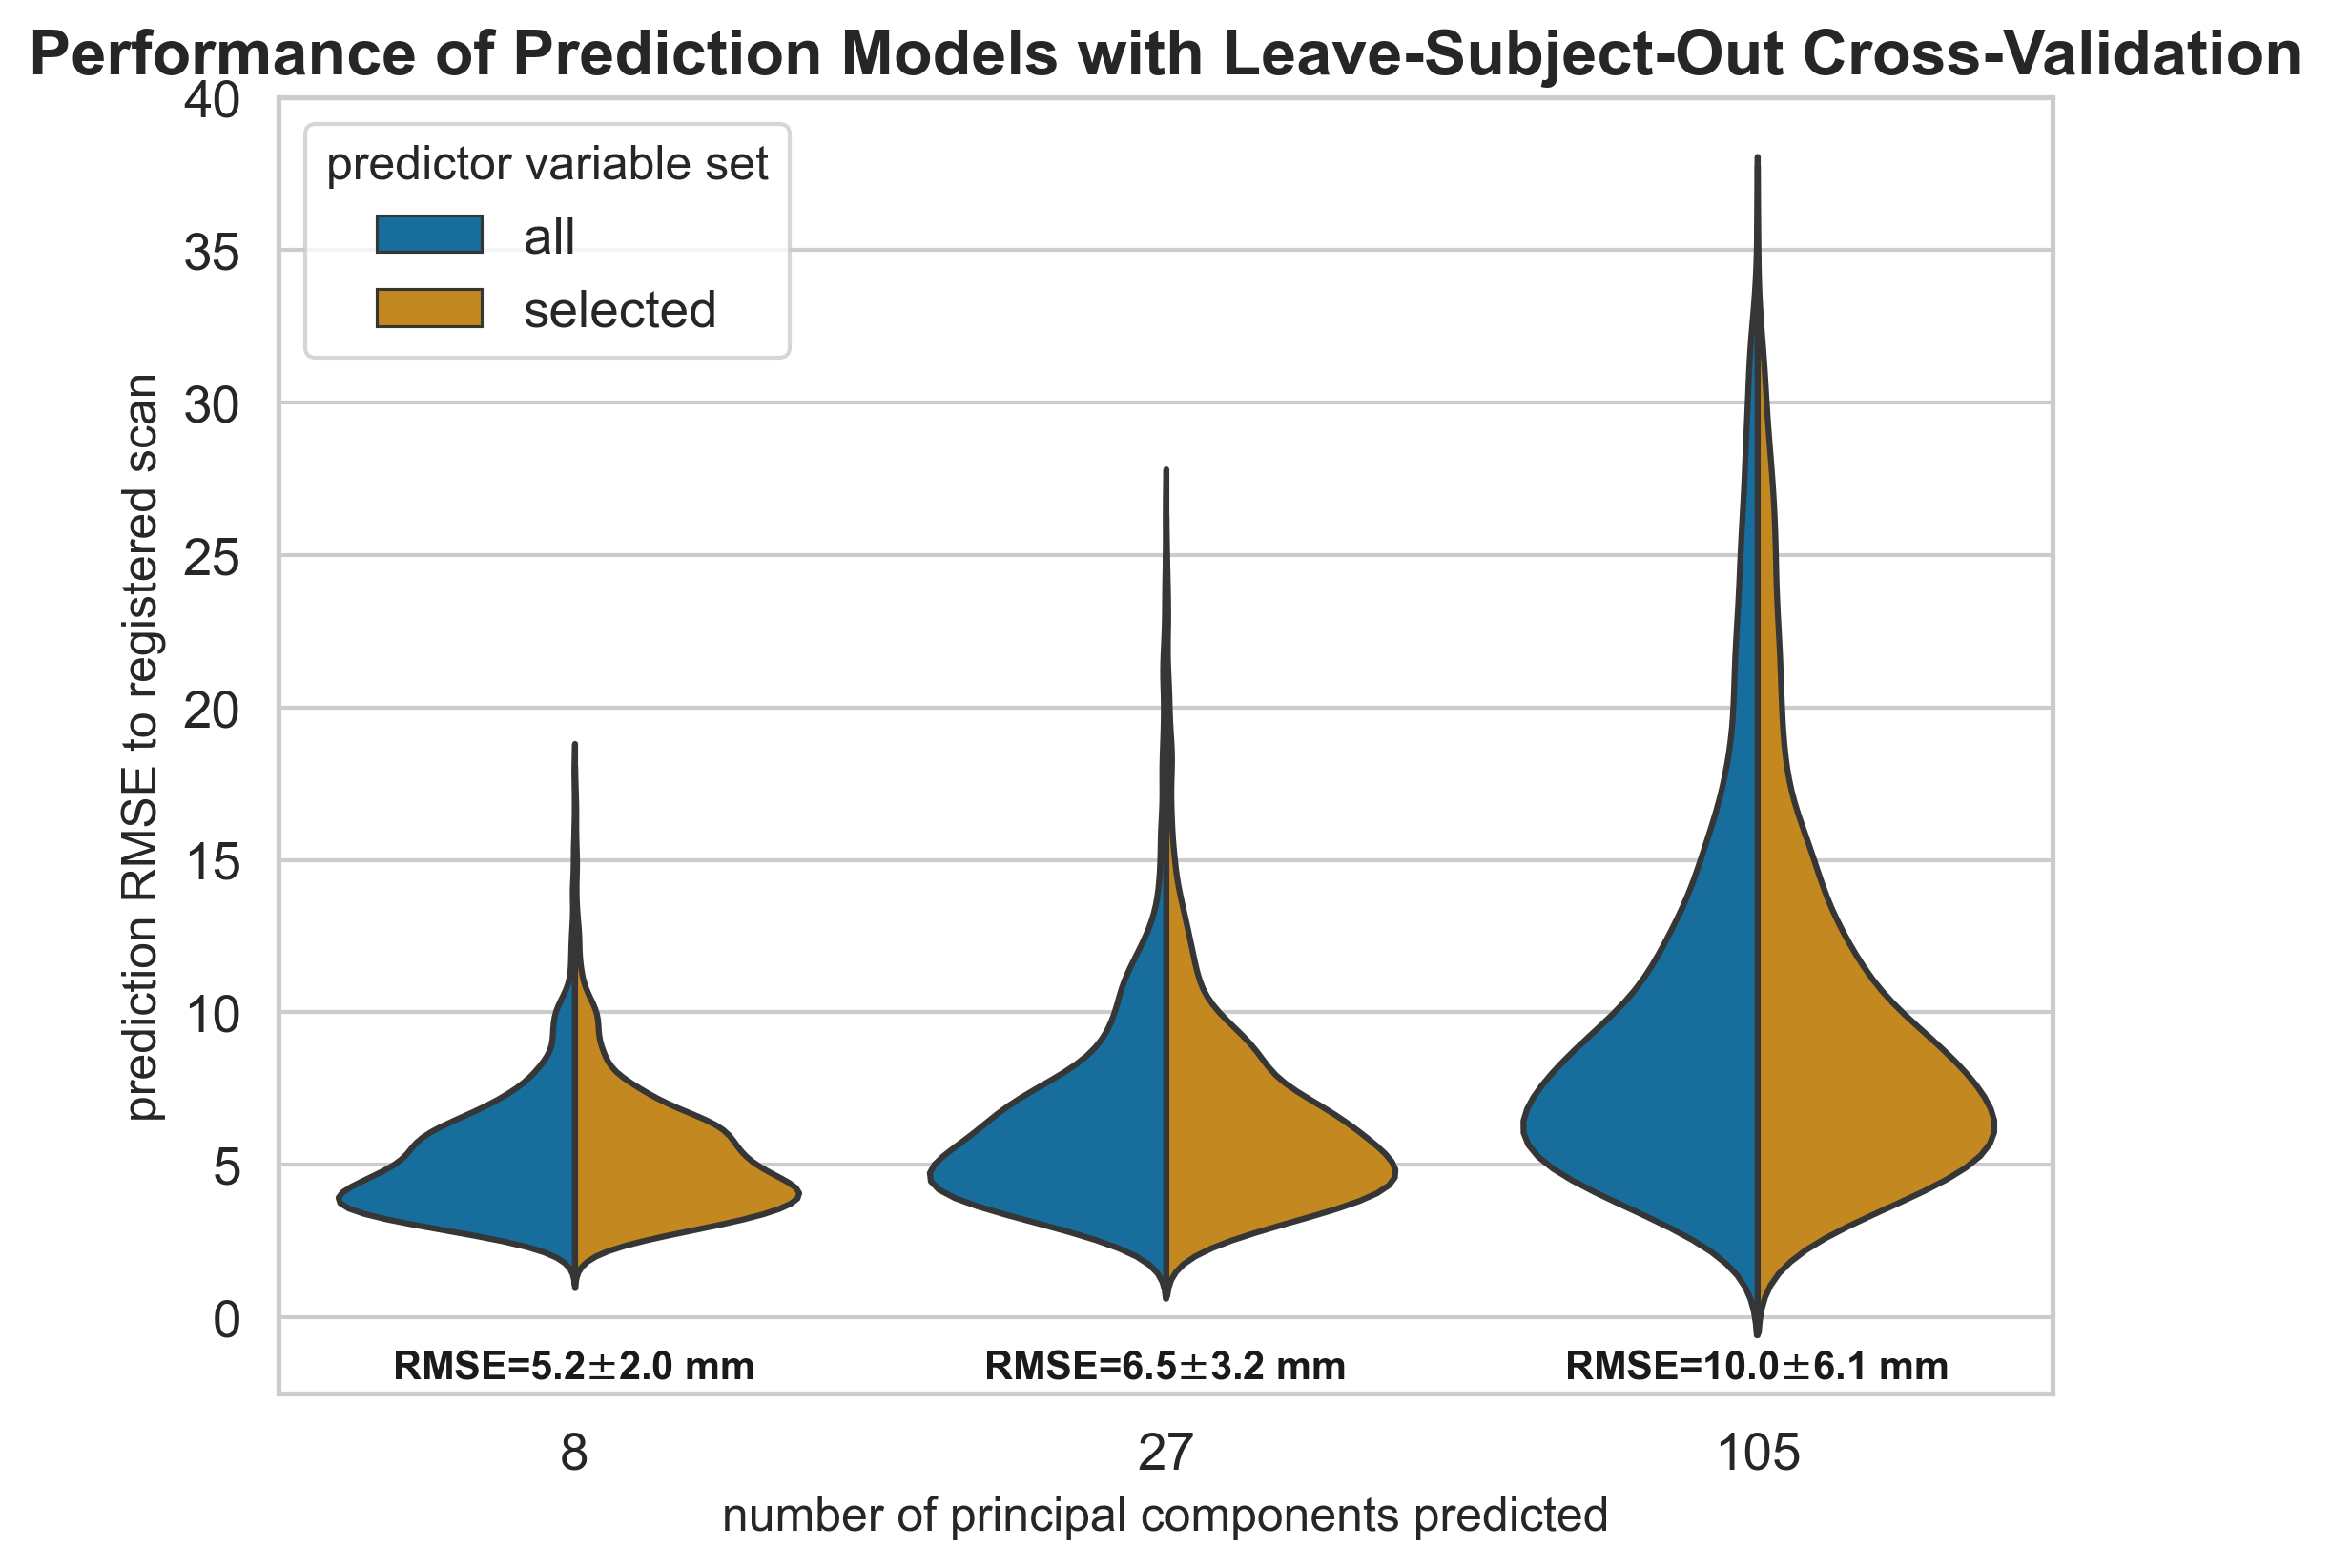
\includegraphics[width=0.8\textwidth,height=\textheight]{../fig/SA2/modelPerformance.png}
\caption{Distribution of errors across the various prediction models leave-subject-out cross-validation results. Model RMSE mean and standard deviation are shown above each distribution.}\label{fig:modelperf}
}
\end{figure}

Each retained PC is a shape mode in the model. Figure \ref{fig:SA2-coefs} shows the chosen model's normalized regression coefficient values for each shape mode.
The coefficients for the sex predictor are not shown as they were calculated to be zero for every shape mode.

\begin{figure}
\hypertarget{fig:SA2-coefs}{%
\centering
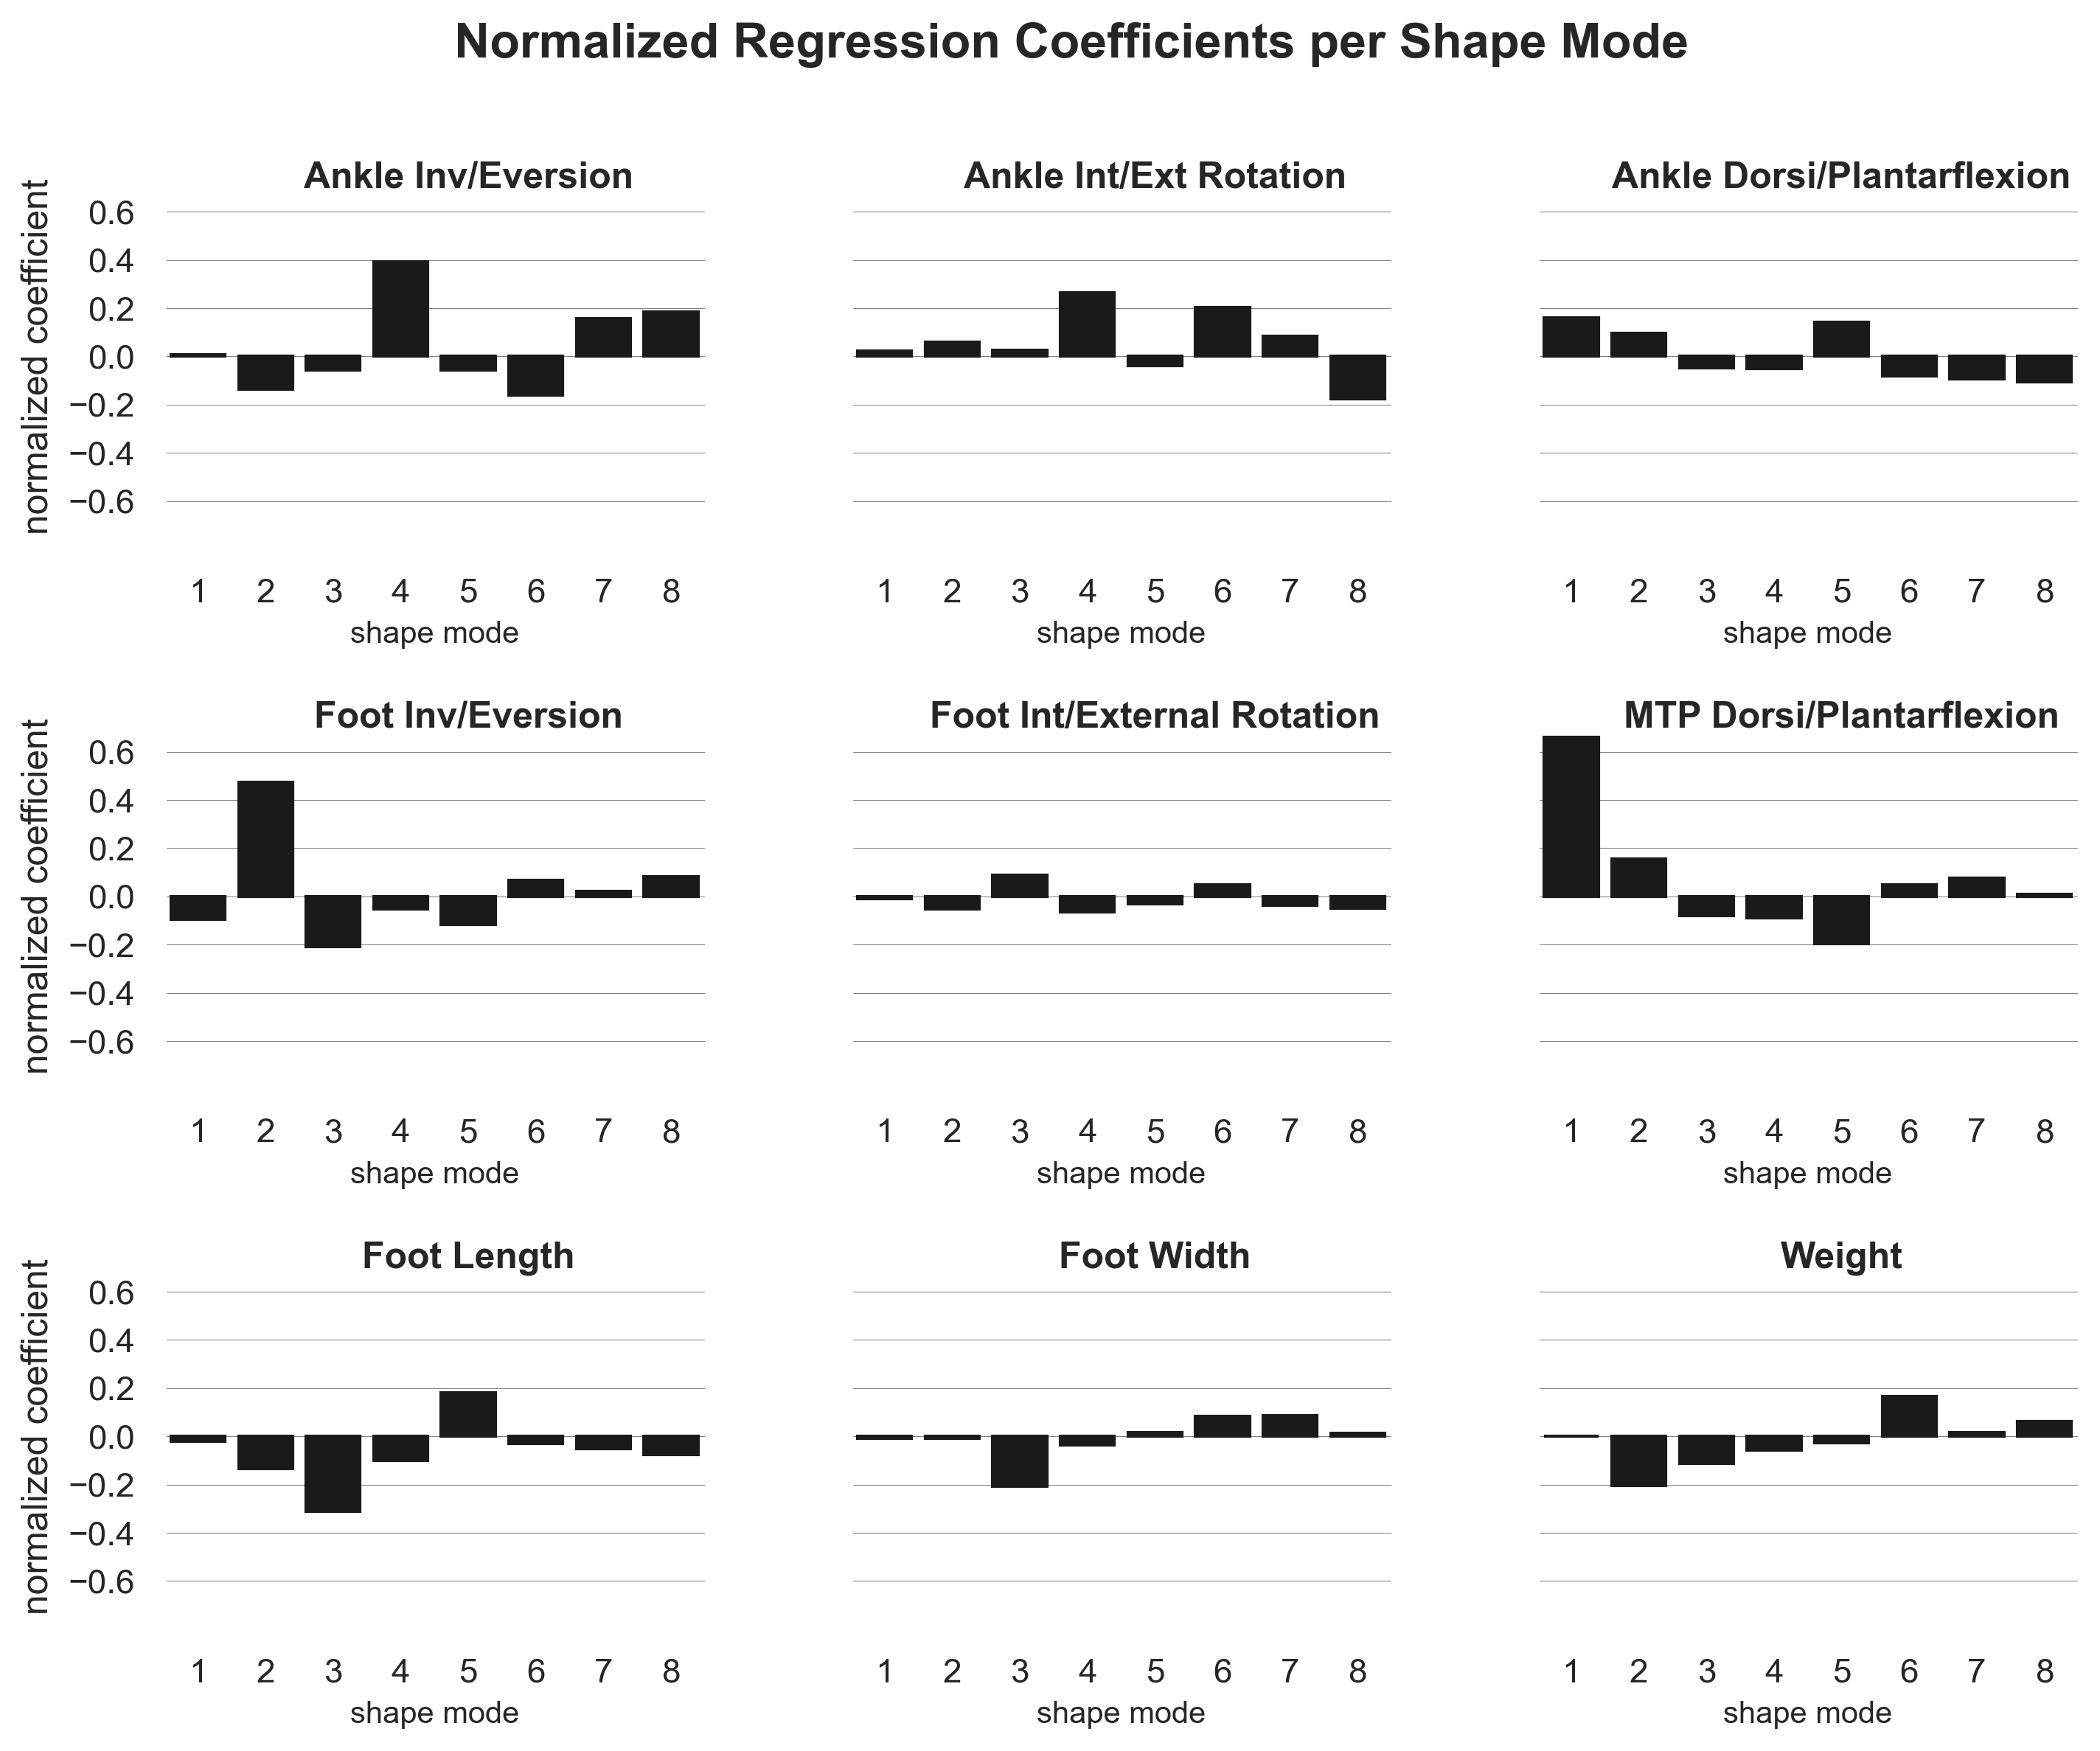
\includegraphics[width=1\textwidth,height=\textheight]{../fig/SA2/coefs.png}
\caption{Each graph represents the predictor's effects on the shape mode by visualizing the model's normalized coefficients. Larger absolute values indicate a larger effect from the predictor on the shape mode.}\label{fig:SA2-coefs}
}
\end{figure}

Figures \ref{fig:pca_all} shows each shape mode's axis represented on the mean foot, highlighting which areas of the foot are affected by deformations in each shape mode, and the \(\pm\) 2 standard deviations of deformation along each shape mode overlaid on the mean foot.

\begin{figure}
\centering

\subfloat[A]{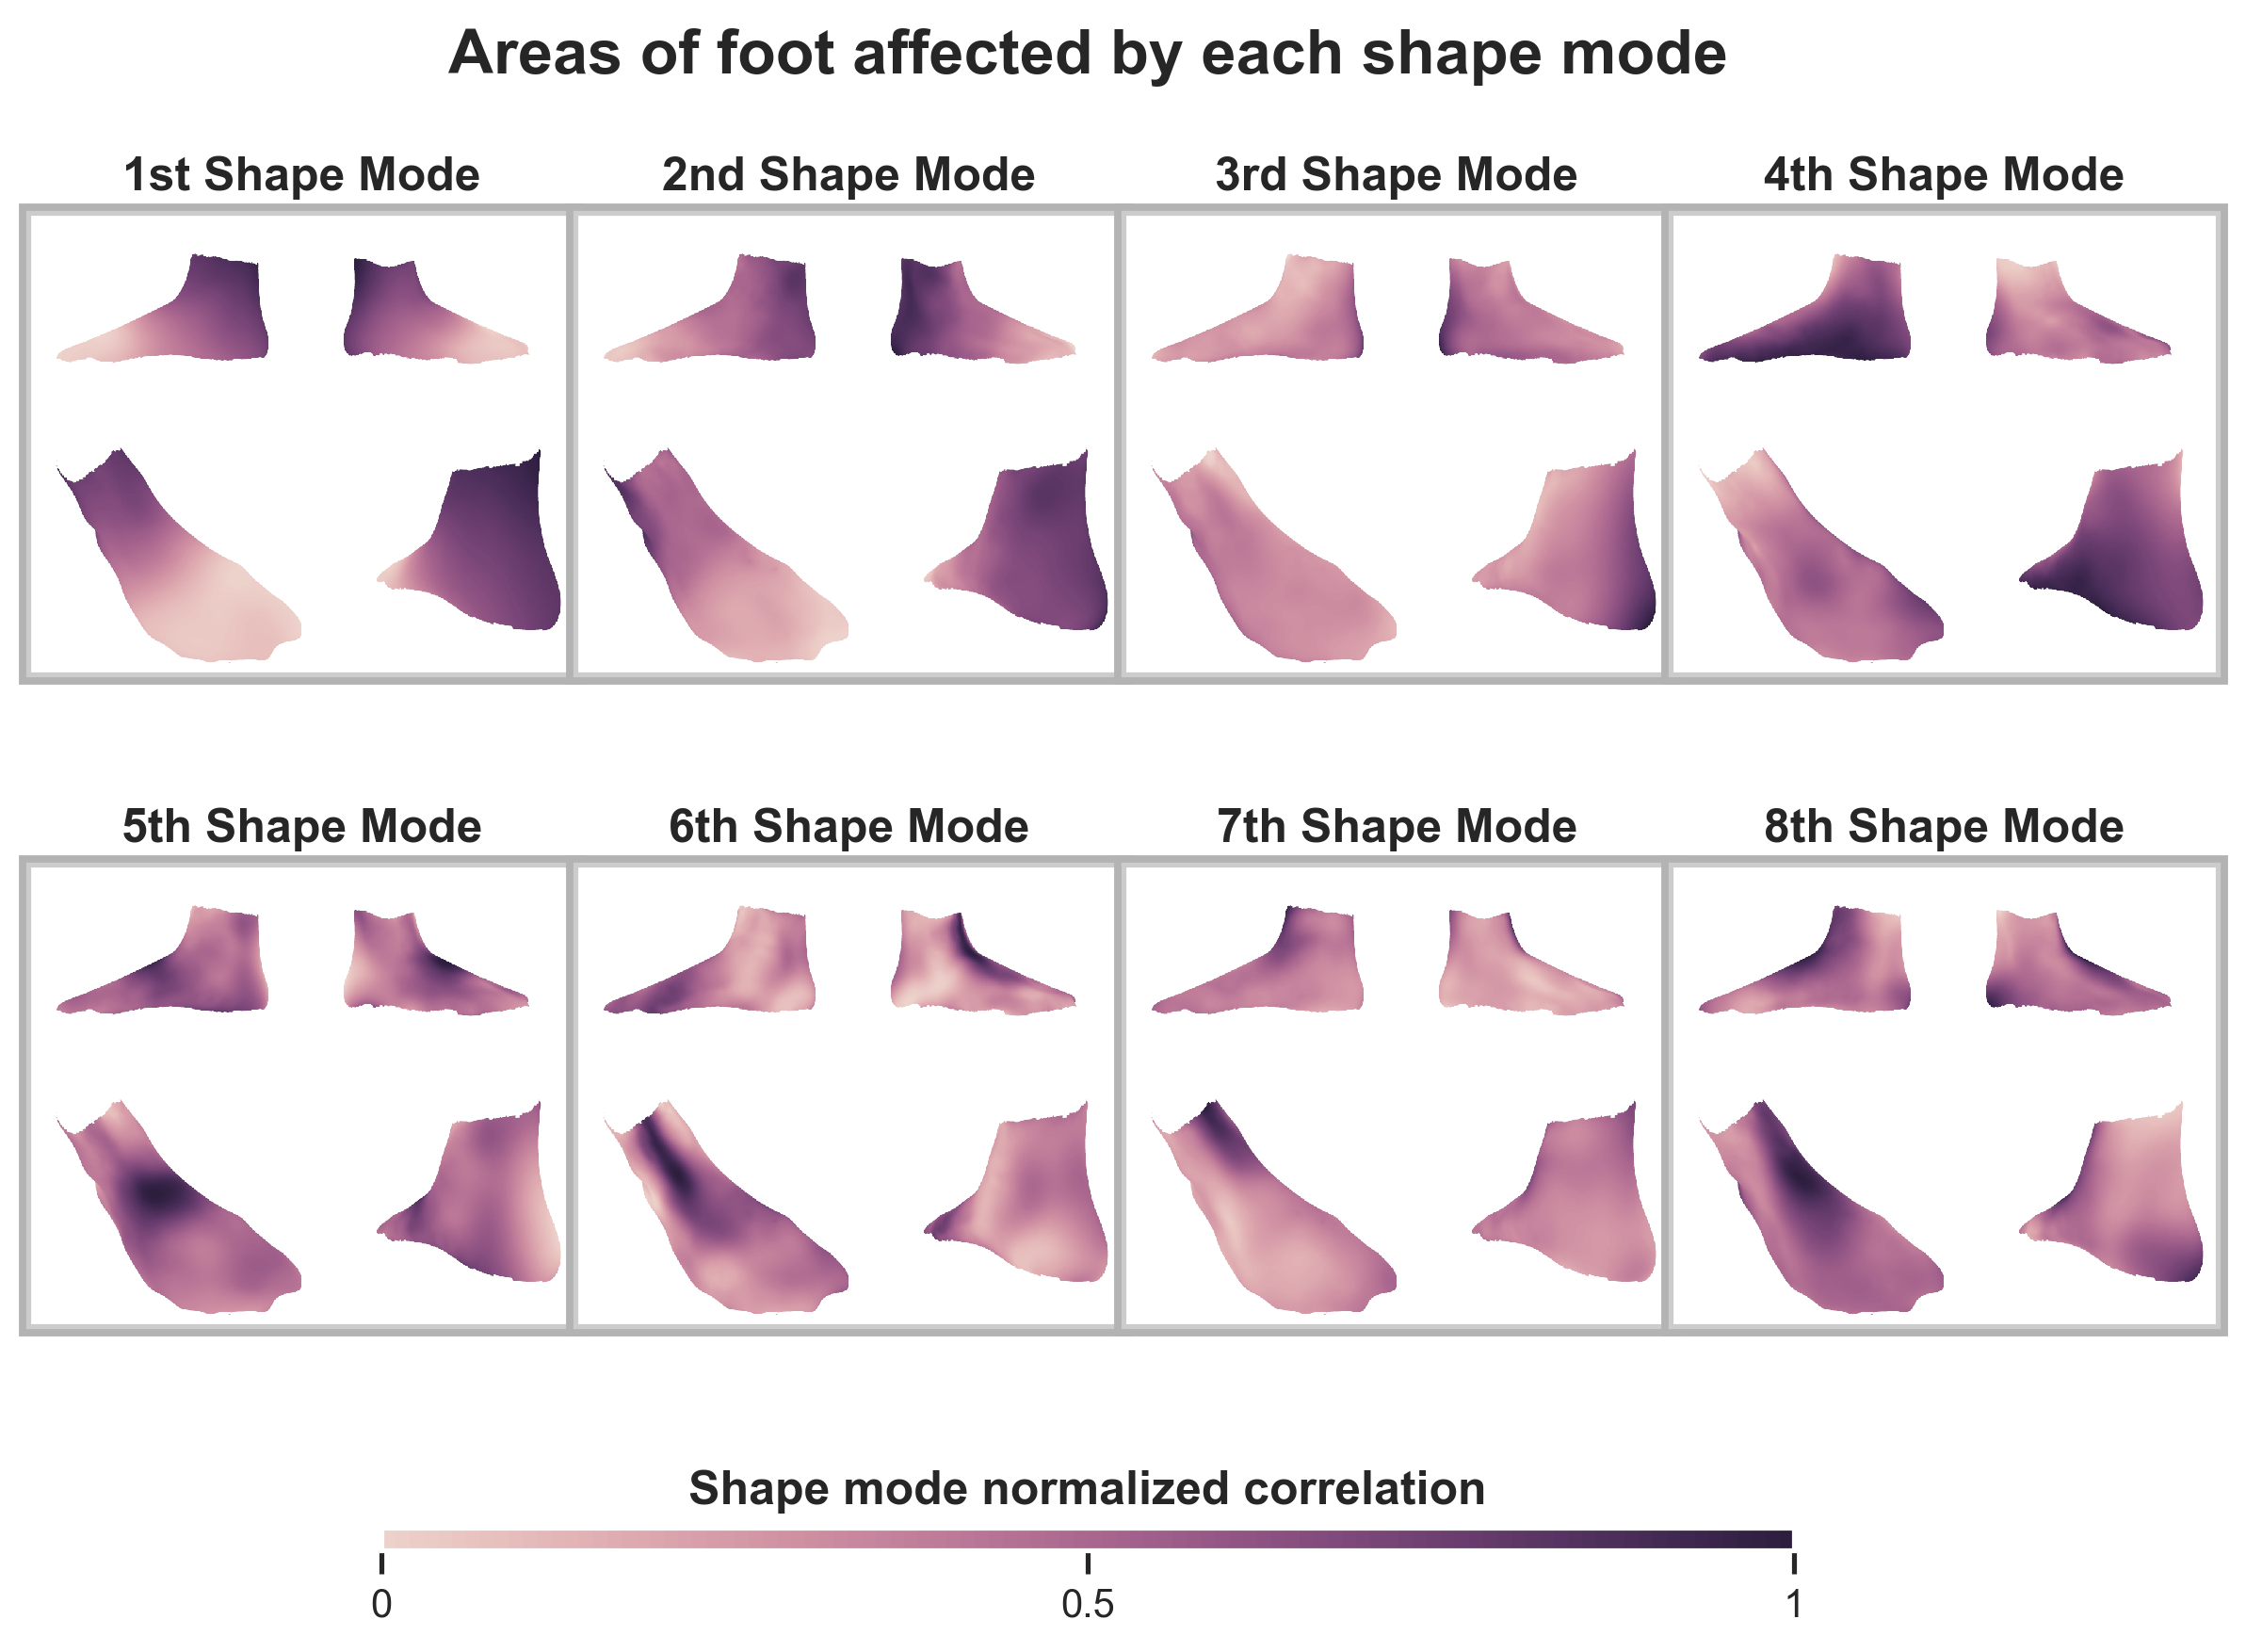
\includegraphics[width=0.8\textwidth,height=\textheight]{../fig/SA2/PCQuad.png}\label{fig:pca_quad}}
\subfloat[B]{\includegraphics[width=0.95\textwidth,height=\textheight]{../fig/SA2/PCVAR.png}\label{fig:pca_overlay}}

\caption{{[}A{]} Each shape mode's principal axis represented as a heatmap overlaid on the mean foot and shown from 4 different point-of-views. The darker regions represent vertices which are most correlated with the shape mode's principal axis, and therefore see deformations in the shape mode. {[}B{]} Foot shape deformation at +2 and -2 standard deviations along each shape mode's principal axis, overlaid on the mean foot. The point-of-view is set to highlight the major variance along each shape mode's axis.}

\label{fig:pca_all}

\end{figure}

This study was designed to construct and evaluate a parametric SSM in explaining and predicting dynamic foot morphology changes across the subject population.
The model was able to predict dynamic foot shape across the subject population with an average RMSE of 5.2 \(\pm\) 2.0 mm. For context, if all possible prediction error was accumulated to only affect length and width, it would be higher than the half-size step of the American shoe sizing system \citep{Luximon2013}, but less than inter-brand variability of shoe length and shoe width \citep{Wannop2019}.
Further, this error is lower than the RMSEs of other parametric SSMs that predicted static standing child body shape (mean=10.4mm) \citep{Park2015a}, dynamic shoulder deformation (mean=11.98mm) \citep{Kim2016} and child torso shape (mean=9.5mm) \citep{Park2017}. Note though, that the presented model may have lower prediction errors due to the foot being a relatively smaller section of the body to model. Grant et al.'s model reconstructed internal foot bones with much lower RMSEs from sparse anatomical landmarks (1.21-1.66 mm for various foot segments) \citep{Grant2020} but was trained with higher resolution MRI images. Other efforts to create statistical foot shape models did not incorporate parametric prediction of foot shape \citep{Conrad2019, Stankovic2020}.

\hypertarget{foot-shape-changes}{%
\subsection{Foot Shape Changes}\label{foot-shape-changes}}

The first, second, and fourth shape modes, accounting for a total of 86.7\% of total variance, capture gross foot motion.
Foot motion during stance is dominated by MTP and ankle dorsi/plantarflexion \citep{Leardini2007}, which is captured in the first shape mode (fig.~\ref{fig:pca_all}).
The second and fourth shape modes capture gross changes in foot rotation from frontal and transverse plane movements at the MTP and ankle joints, respectively (fig.~\ref{fig:pca_all}).
The second shape mode is most affected by foot inversion/eversion around the MTP joint.
The second shape mode also captures girth scaling at the ankle joint, as seen in (fig.~\ref{fig:pca_all}) by how the ankle girth decreases along the axis, and is affected by weight (fig.~\ref{fig:SA2-coefs}).
The fourth shape mode is affected by ankle inversion/eversion and internal/external rotation.
Foot inversion/eversion, ankle inversion/eversion, and ankle internal/external rotation are expected to vary across the stance phase (\citep{Leardini2007}), which leads to the observed changes in gross movement.
However, the second and fourth shape modes are slightly affected by foot length, which may suggest inter-individual effects in foot inversion/eversion, ankle inversion/eversion, and internal/external rotation during gait.
There is a slight correlation between these angles and foot length (see supplementary figures), which may be due to differences in cadence when walking at the treadmill's set speed.
Individuals were given time to acclimate to the treadmill's set speed, but the speed may not have been their preferred walking speed.

The third shape mode captures foot shape scaling at the rearfoot, as highlighted in (fig.~\ref{fig:pca_all}).
Foot length shrinks when moving positively along the third shape mode (fig.~\ref{fig:pca_all}), and thus has a negative effect from foot length.
There are also negative effects from foot width and weight, which may be due to their correlation to foot length (see supplementary figures).
Rearfoot morphology along this shape mode has a more rounded shape in the negative direction, and a sharper shape in the positive direction (fig.~\ref{fig:pca_all}).
There is also a negative effect from foot inversion/eversion (fig.~\ref{fig:SA2-coefs}), indicating that with foot eversion, a sharper rearfoot shape is expected.
This may be due to foot eversion at heel-off \citep{Leardini2007}, where the foot unloads from a rounder weight-bearing rearfoot to a sharper non-weight bearing rearfoot shape.

Midfoot girth increases and the rearfoot is rounder along the fifth shape mode's axis (fig.~\ref{fig:pca_all}).
The fifth shape mode is positively affected by foot length and negatively by MTP dorsi/plantarflexion (fig.~\ref{fig:SA2-coefs}).
This suggests that static midfoot girth increases with foot length, and decreases through heel-off as the MTP dorsiflexes.
Rearfoot morphology is rounder for longer foot lengths but gets sharper through heel-off with MTP dorsiflexion, much like in the third shape mode.
Midfoot girth was previously found to decrease during stance phase compared to statically standing \citep{Grau2018}, most likely due to intrinsic and extrinsic foot muscle contraction \citep{Scott1993, Gefen2000}.
However, it was not noted where during stance phase midfoot girth decreases, but it can now be assumed it occurs during heel-off.

The sixth shape mode captures girth changes at the ankle, midfoot, and the medial MTP joint region (fig.~\ref{fig:pca_all}), with girth increasing along the axis.
There are positive effects from ankle internal/external rotation and weight, while there is a negative effect from ankle inversion/eversion ({[}fig:SA2-coefs{]}).
Static MTP, midfoot, and ankle girth may therefore increase with subject weight.
Dynamic girth changes in these regions may occur as the ankle everts and internally rotates just prior to toe-off, where muscle activation is needed to push the foot off the ground.
The foot is stiffened through tension in the MTP joints in order to prepare for toe-off \citep{Hicks1954}, and the MTP joints are known to move relatively within the foot during gait \citep{Wolf2008, Lundgren2008} which may be resulting in the increased girth at the MTP joint.
A similar mechanism may be occurring at the ankle joint during ankle inversion and internal rotation, where tension from muscle activation prior to toe-off may cause increased girth.

The seventh and eight shape modes, accounting for 1.3\% of total variance, capture girth increases near the medial malleolus along their axes (fig.~\ref{fig:pca_all}).
They are both positively affected by ankle inversion/eversion (fig.~\ref{fig:SA2-coefs}), and the eight shape mode is further negatively affected by ankle internal/external rotation.
This may suggest that the girth around the medial malleolus decreases prior to push-off, as the ankle everts and internally rotates.

\hypertarget{study-limitations}{%
\subsection{Study Limitations}\label{study-limitations}}

A number of limitations in this study should be noted.
The elastic-net method is able to retain cross-correlated predictors, but still requires some bias in the dataset to predict scenarios where cross-correlated predictors are independent \citep{Zou2005}.
Therefore, the presented model may not be valid for predicting changes in morphology due to independent changes in joint angles outside of stance phase, or for variance in foot width or weight compared to foot length not captured in the subject population.

The model did not capture differences between male and female feet.
Studies found that sex differences in foot shape after scaling for foot length were not significant \citep{Kouchi2009, Barisch-Fritz2014a, Conrad2019}, or were small in magnitude \citep{Wunderlich2001, Krauss2008}.
No subject demographic data was collected to account for differences in foot shape due to ethnicity \citep{Jurca2019}.
No data was captured on the foot's plantar surface due to limitations with the scanning system; therefore foot arch changes were not captured.
Data captured around the toes had high noise, which necessitated smoothing the toes in the template to ease fitting.
Future advances in 4D scanning may alleviate some of these concerns, and also allow for expansion of this model to higher frequency foot motions, such as running.

\hypertarget{study-conclusions}{%
\subsection{Study Conclusions}\label{study-conclusions}}

The observed girth changes at the ankle joint, medial malleolus, midfoot, and MTP joint can be directly mapped to spacesuit footwear design recommendations to reduce instances of heel-lift.
During heel-lift, the heel rises inside the boot, resulting in the midfoot rotating upward around the MTP-joint much like after the heel-off phase in gait.
This can only occur if there is empty space above the midfoot; if the boot's internal shape were perfectly fit to the foot's shape, the foot would not be allowed to move inside the boot.
Unlike some terrestrial footwear which can rely on the elasticity of uppers to continuously capture the foot, the stiff nature of a pressurized spacesuit boots does not allow for its upper to continuously conform to the foot if the foot changes shape.
The study showed that midfoot girth decreased as the MTP joint is dorsiflexing after heel-off in the fifth shape mode.
Therefore, a spacesuit boot should have a mechanism to conform to this volume change to reduce empty space above the midfoot and therefore reduce instances of heel-lift.
Heel counters are also designed into many terrestrial boots to ensure the heel stays index through motion; a well-designed heel-counter could also help reduce heel-lift.
Rearfoot morphology changed from a rounded shape to a sharper shape with MTP joint dorsiflexion in the fifth shape mode, suggesting that a heel-counter may need to account for this shape change to properly capture the heel.
A combination of midfoot capture and an improved heel-counter that account for these morphological changes can work together to reduce instances of heel-lift in the spacesuit boot.

\hypertarget{instep-height-and-girth-analysis}{%
\section{Instep Height and Girth Analysis}\label{instep-height-and-girth-analysis}}

While the dynamic foot shape model provides insight into how regions of the foot change shape due to motion or anthropometry, it only outputs foot shapes and not linear or circumferential foot measurements.
One of the primary findings in this study was the decrease in midfoot girth through heel-off; this region is represented by the linear foot measurements of instep height and instep girth.
Translating the foot-shape changes in the midfoot to linear measurements will provide a basis for footwear designers to ensure their uppers have the range to conform to the midfoot throughout gait.
Specifically for this thesis, this linear measurement will provide a baseline for engineering a conformable upper into a spacesuit boot to reduce empty space above the midfoot and thereby reduce heel-lift.
In addition, comparing dynamic changes in these measures to their static population range will allow for future sizing analyses to include how much instep height conformal range is needed for each shoe size.

Volumental AB, a footwear research company, has developed a database of 1.2 million footwear consumer static foot scans around the world \citep{Jurca2019}.
Analysis of this database showed that static instep height in the median 90\% of the population had a range of 16.2 mm \citep{Jurca2019}.
In collaboration with Volumental AB, The dynamic foot shape model will be expanded to output instep height measurements, with the method outlined in Jurca et al. \citep{Jurca2019}, across the kinematic variables, foot length, and foot width of the dynamic model's subject population.
When compared to the static measurements done by Jurca et al. \citep{Jurca2019}, tolerances for instep height can be defined across the population; specifically, the range needed to capture the median 90\% population for each foot length class.
In this thesis, and in collaboration with Volumental AB, these results will be extended to instep girth.
Findings from this study will be related to spacesuit design variables.

As a stretch goal, this analysis can be repeated for the measures of foot length, foot width, and heel width.
While this goal is not a thesis contribution, this opens the door to understanding how foot much footwear needs to be conformal to the user's foot shape; identifying variables that will help prioritize footwear design measures.

\hypertarget{summary-3}{%
\section{Summary}\label{summary-3}}

A 4D scanning system was developed to capture dynamic foot shape changes, and was used to collect data for development of the model.
To the authors' knowledge, this is the first parametric foot SSM that captures and reconstructs dynamic motion.
The model was able to identity specific changes in foot morphology as they related to subject and kinematic parameters, and suggest spacesuit boot design techniques to reduce instances of heel-lift.
Along with these techniques, the model is able to reconstruct a full 3D model when parameter values are provided, which offers a design starting point for constructing a planetary spacesuit boot prototype in Specific Aim 3.

To date, all data-collection for Specific Aim 2 has been completed.
A journal paper detailing the development of the 4D scanning system was published in the Journal of Open Source Software \citep{Boppana2019}.
A journal paper detailing the development of the model is currently under review, and has been released as a preprint \citep{Boppana2020b}.
The instep height and instep girth analysis is just starting and will be presented in a future journal paper.

\hypertarget{specific-aim-3-define-a-design-process-integrating-dynamic-foot-morphology-data-for-a-novel-spacesuit-boot}{%
\chapter{Specific Aim 3: Define a design process integrating dynamic foot morphology data for a novel spacesuit boot}\label{specific-aim-3-define-a-design-process-integrating-dynamic-foot-morphology-data-for-a-novel-spacesuit-boot}}

\hypertarget{introduction-2}{%
\section{Introduction}\label{introduction-2}}

The design for any new spacesuit component should aim to match the required operator motions for the intended actions, as well as be sized for the intended population.
This allows for the component to provide proper fit and mobility to the wearer, but proper design requires an understanding of body segment size and mobility.
Planetary spacesuit boots have previously started out with modifying terrestrial hiking boot designs to be pressurized, and then designed through iteration and subjective feedback.
To date, these designs have failed to solve the heel-lift problem, necessitating a new approach to boot design.
Combining the novel dynamic foot morphology model with known foot shape and mobility characteristics provides the necessary information to better fit the spacesuit boot to the foot.
However, there is not a clear process for integrating all available data to drive spacesuit component design with a focus on improved fit and mobility.
This object aims to define that process specifically for the spacesuit boot, through the following objectives:

\begin{itemize}
\tightlist
\item
  Literature review of existing foot shape and mobility knowledge
\item
  Development of a design framework to design a more compatible spacesuit boot
\item
  Design and construction of a spacesuit boot prototype leveraging the design framework
\end{itemize}

\hypertarget{existing-knowledge-on-foot-shape-mobility}{%
\section{Existing Knowledge on Foot Shape Mobility}\label{existing-knowledge-on-foot-shape-mobility}}

The foot's static shape distribution and mobility have been well characterized through previous analyses \citep{Farris2019, Mann1979, Voloshina2013, Wannop2014}.
The following sections describe each of these specific foot measures and provide their population-derived nominal values.
Figure \ref{fig:SA3-Foot} highlights these foot-specific measures.

\begin{figure}
\hypertarget{fig:SA3-Foot}{%
\centering
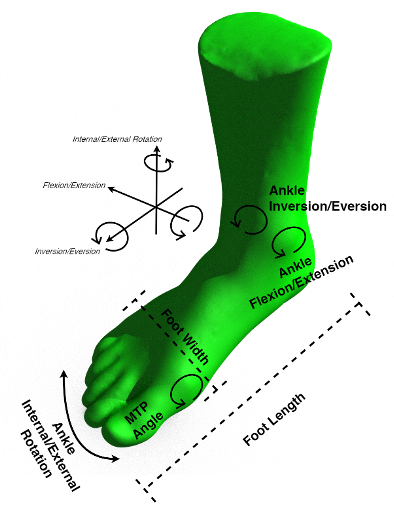
\includegraphics[width=0.4\textwidth,height=\textheight]{../fig/SA3/FootOverview.png}
\caption{Foot-specific measures which directly affect mobility and comfort}\label{fig:SA3-Foot}
}
\end{figure}

\hypertarget{linear-anthropometry}{%
\subsection{Linear Anthropometry}\label{linear-anthropometry}}

The ANSUR II survey collected a number of foot-related measures which can be analyzed to provide a baseline for foot shapes and sizes\citep{Gordon2014}.
Three of these measures are directly related to fit and mobility.
Foot length and foot width define the outer bounds of the foot shape.
Foot length and width are directly correlated to US shoe sizes for both width and length.
Since females generally feature smaller feet than males, female shoe size is typically 1.5 units less than the calculated male size.
Figure \ref{fig:SA3-ANSUR} shows that this offset does not sufficiently align the female population to the male population.
Therefore, it is important to use foot length as a direct measure when fitting or selecting a shoe as opposed to shoe size.

Arch length denotes the location of the metatarsophalangeal (MTP) joints on the foot, one of the important joints during gait.
Since power is transmitted through the MTP joints, the alignment of the MTP joints with the ball of the shoe is important to ensure power is properly transmitted during heel-off.
Therefore, the arch length measurement is correlated to standard shoe sizes and if larger, will be selected over the length measurement.
Figure \ref{fig:SA3-ANSUR} shows that while arch length is correlated to foot length for both males and females, there is still high variability in this relationship.
Therefore, arch length is an important measure to consider to ensure proper indexing and dynamic fit between the wearer and spacesuit boot.

\begin{figure}
\hypertarget{fig:SA3-ANSUR}{%
\centering
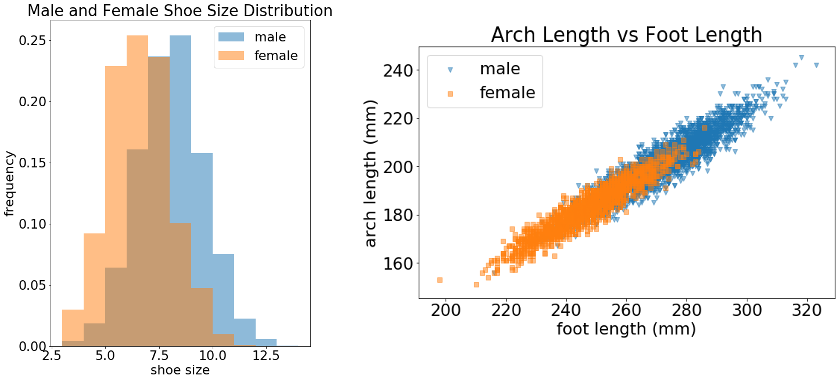
\includegraphics[width=0.8\textwidth,height=\textheight]{../fig/SA3/ANSUR.png}
\caption{(Right) Inequality in distribution of equivalent shoe size between male and female, (Left) relationship between foot length and arch length; visualizations developed from the ANSUR II Dataset}\label{fig:SA3-ANSUR}
}
\end{figure}

\hypertarget{gait-joint-kinematics}{%
\subsection{Gait Joint Kinematics}\label{gait-joint-kinematics}}

The foot's main function during gait is to transmit power against the ground, ensuring that the human pushes off and initiates a step.
During each step, the ankle pushes off from the ground to initiate a step.
Intrinsic foot muscles help stiffen the foot to assist the push-off from the ankle against the ground \citep{Farris2019}.
The MTP joint not only exhibits flexion in the sagittal plane, but provides the necessary stiffness to allow for the ankle power to translate into push off \citep{Stefanyshyn1997}.
Ankle joint rotation may also help balance and stability during gait, particularly on slopes \citep{Wannop2014}. Neither the ankle joint nor the MTP joint should be restricted in its movement to enable efficient push-off and stability.
However, free movement of the ankle joint can increase the risk of injury from instability caused by external forces from walking on an uneven surface.
Therefore, there is a balance to be struck between allowing for movement while preventing potentially injurious movements.

Nominal values for the foot MTP and ankle joint movement during gait can be derived from the numerous studies conducted on human gait.
Voloshina et al. \citep{Voloshina2013} found that during gait on uneven surfaces, the ankle does not flex past +/- 20 degrees.
Wannop et al. \citep{Wannop2014} reported peak foot-floor angles which suggest that on level and sloped surfaces, subjects dorsiflex their ankle up to 40 degrees, and flex their MTP joint up to 60 degrees.
The MTP joint has been shown to flex between 70-90 degrees during gait \citep{Mann1979}.
There is very little ability of the MTP joint to extend or move in the frontal or transverse plane \citep{Mann1979}; therefore these motions may want to be limited in the boot's design to prevent injury.

The ankle joint exhibits most of its movement in the sagittal plane.
However, the ankle joint can perform inversion/eversion in the frontal plane and internal/external rotation in the transverse plane.
Wannop et al. \citep{Wannop2014} found that subjects wearing a low-top shoe with no additional ankle stability had up to 10 degrees eversion and 15 degrees inversion while navigating a slope.
However, excessive inversion/eversion may decrease stability and lead to injury.
During gait, the human normally exerts energy to stabilize their ankle in this direction \citep{OLoughlin2009}.
However, any external force can destabilize the ankle, as commonly seen in basketball or hiking \citep{Bohm2010}.
Therefore, it will be desired that any boot stabilizes the ankle in this motion.
In addition, freedom in the transverse plane is desired to allow for positioning of the foot when navigating an uneven surface, aiding in balance \citep{Wannop2014, Fraser2016a}.
Wannop et al. \citep{Wannop2014} found the ankle internally/externally rotates +15/-20 degrees on a slope.

\hypertarget{biomechanical-boot-design-framework}{%
\section{Biomechanical Boot Design Framework}\label{biomechanical-boot-design-framework}}

The proposed design framework will link foot measurements described in the previous section and the dynamic foot shape model to specific footwear design variables, allowing for the design of a spacesuit boot with proper fit and mobility.
The framework assumes the development of a gas-pressurized spacesuit boot to maintain compatibility with the current xEMU architecture.
Since gas pressurized spacesuits are stiff when pressurized, they require specially designed joints which allow for flexibility of the stiff structure.
The gas pressurized layer does not have the ability to stretch once pressurized, and therefore must be sized specifically to fit the population range.

Footwear design variables are categorized as either population measures or individual measures.
Population design variables are used in the general design and selections of materials for the shoe, which will accommodate the range of foot shapes and motions seen by the population.
Individual design variables will be sizing specific elements which are changed between sets of boots to fit inter-individual differences (such as shoe size).
Foot mobility measures are used to define the range-of-motion of the boot's joints.
Foot shape measures can be used to shape the upper and sole of the boot, aiming to accommodate the foot shape inside.
Sizing variables such as foot length, foot width, and arch length, are used to influence the size of the components developed from foot mobility and foot shape measures.
Figure \ref{fig:SA3-Overview} shows how each of these measures is mapped to footwear design variables.

\begin{figure}
\hypertarget{fig:SA3-Overview}{%
\centering
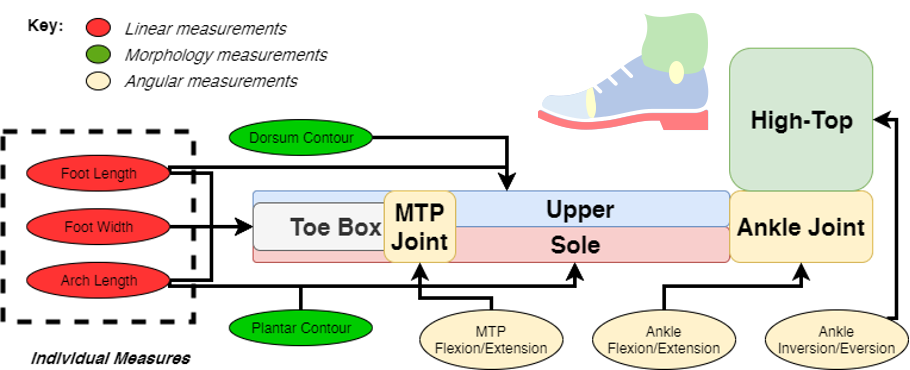
\includegraphics[width=0.9\textwidth,height=\textheight]{../fig/SA3/Overview.png}
\caption{Overview and classification of measurements to footwear design variables with representative shoe}\label{fig:SA3-Overview}
}
\end{figure}

\hypertarget{mobility}{%
\subsection{Mobility}\label{mobility}}

Footwear is flexible at the MTP and ankle joints to allow for effective push-off during gait. Terrestrial footwear normally derives flexibility from the materials used for that portion of the shoe; the shoe is typically made of softer materials or less reinforcement at the joints. Since altering materials property stiffness is not an option for spacesuit design, rolling convolute or toroidal joints could be used in the spacesuit footwear to allow for flexibility at the MTP and ankle joints \citep{Harris2001}. fig.~\ref{fig:SA3-Mobility} shows the desired flexibility based on foot-specific measures. These population measures will ensure that the boot provides enough flexion to not constrict natural motion.

The MTP joint should target flexion of +90 degrees and the ankle joint should target dorsiflexion/plantarflexion of +40/-20 degrees.
Due to the potential for unstable terrain, a high top style footwear is suggested to stabilize the ankle, similar to a hiking or military style boot.
However, it has been shown that a very stiff boot reduces ankle ROM and decreases stability at the knee joint \citep{Bohm2010}, potentially leading to ankle and knee fatigue.
By allowing for a internal/external rotation of +15/-20 degrees, and inversion/eversion of +15/-10 degrees, the boot still allows the foot to navigate a sloped and uneven surface without fatigue.
The relatively low amount of movement will still allow the ankle to be stabilized and lower the risk of injury.

The only requirements previously stated for boot mobility are in the 2019 NASA SBIR Surface Space Suit Boot Solicitation \citep{NASA2019}.
The solicitation matches the +40/-20 degrees ankle dorsiflexion/plantarflexion requirement, but presents no requirements for ankle internal/external rotation, inversion/eversion, or MTP joint flexion.
The proposed design framework targets higher flexion/extension capability in the ankle joint, as well as specifies extension of the MTP joint, limited ankle internal/external rotation, and limited ankle inversion/eversion.

\begin{figure}
\hypertarget{fig:SA3-Mobility}{%
\centering
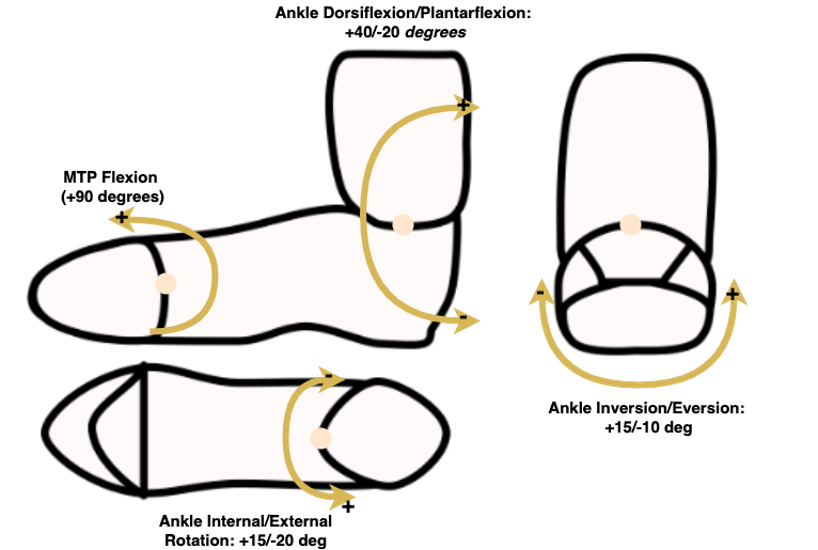
\includegraphics[width=0.6\textwidth,height=\textheight]{../fig/SA3/Mobility.png}
\caption{Mobility and flexibility of joints needed in the spacesuit boot}\label{fig:SA3-Mobility}
}
\end{figure}

\hypertarget{toe-box}{%
\subsection{Toe box}\label{toe-box}}

The toe box accommodates the foot forward of the MTP joint.
The toes provide the contact for power from the MTP and ankle joints to push off the ground during each step.
Therefore, the most important feature of the toe box is contact between the toes and the ground during heel-off.
As a result, the toe box can feature more space around the top of the toes for comfort \citep{Luximon2009}.
Since the toe box does not need to provide any additional flexibility, it can be constructed with a less flexible material to allow for adequate support of the boot and foot.
In conjunction with the MTP joint, the toe box should also be adjustable such that it can match the arch length of the wearer, allowing for proper fit and indexing of the MTP joint.

\hypertarget{upper}{%
\subsection{Upper}\label{upper}}

The dorsum of the foot is covered by a shoe upper.
The shape of the upper needs to conform to the shape of the dorsum to allow for proper driving of the shoe during any activity \citep{Feeney2019}.
Foot shape data taken from a large population will be useful in defining an ideal upper shape that fits a range of persons.
The boot upper will also have to conform to the foot shape without causing discomfort during movement.
Dynamic foot shape data can quantify how dorsum shape is changing throughout the gait cycle, allowing for the upper to accommodate any expansion or contraction of the dorsum shape for optimal comfort and support.
The dynamic foot shape model drive the design of an upper which can be easily scaled to different shoe sizes.

The upper's location between the MTP and ankle joint, and its requirement to conform to the shape of the foot, drive the selection of a softer, flexible fabric being used to meet these requirements.
This presents a challenge with designing the pressure bladder, as the pressure bladder is inherently stiff under pressure.
Therefore, a soft inner layer above the dorsum may be used which allows the stiff pressurized bladder to conform to the individual's dorsum.
Since the dorsum still transmits power to push the shoe off the ground, the soft layer still needs to have enough structure to transmit this power.
If too soft, the layer will simply act as empty space and the shoe will not respond to ankle flexion during heel-off, potentially resulting in heel-lift.
Lacing or other closure mechanisms would further allow the shoe upper to conform to the dorsum and capture the foot.
Furthermore, the closure mechanism should be customizable by the individual wearing the boot, so each wearer can adjust to where they feel is comfortable.
Conforming the upper to the dorsum will also eliminate any empty space between the foot and above the dorsum, reducing the chance of heel-lift since the foot will no longer be allowed to move within the boot.
In addition, this reduces the chance of contact injuries from rubbing between the foot and boot.

The upper will also play a role in donning and doffing of the spacesuit boot.
Traditional boots feature laces along the upper which secure the foot inside the boot during activity, but loosen to allow the foot to slip into and out of the boot.
The closure can be designed in conjunction with a single structured fold in the pressure bladder to allow the pressure bladder to change shape and allow the foot to be released from the boot.
Figure \ref{fig:SA3-Upper} shows a possible configuration of the upper using laces which conforms to the shape of the foot while still allowing for donning and doffing.

\begin{figure}
\hypertarget{fig:SA3-Upper}{%
\centering
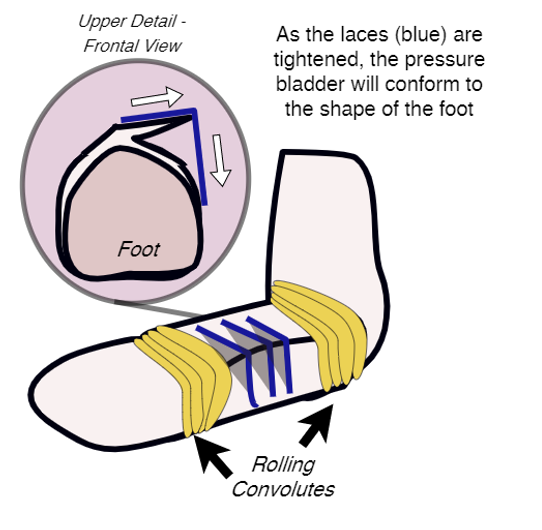
\includegraphics[width=0.5\textwidth,height=\textheight]{../fig/SA3/Upper.png}
\caption{Conceptual design of a boot's upper configuration with pressure bladder}\label{fig:SA3-Upper}
}
\end{figure}

\hypertarget{sole}{%
\subsection{Sole}\label{sole}}

The sole in a traditional boot provides traction, support, and protection to the wearer.
The sole needs some thickness to accommodate tread for grip on uneven surfaces.
In general, the thicker a sole, the stiffer it becomes.
As a stiff sole resists bending, it might fight against the motion of the foot and shoe during heel-off.
Therefore, the sole needs to be flexible during heel-off without imparting additional forces on the shoe and upper.
Dobson et al. \citep{Dobson2020} found that having a fully flexible sole in coal miner's boots inhibited the natural roll-off of the foot during gait, resulting in less comfort.
However, it was not verified if the boot's flexibility at the MTP joint aligned well with the MTP joint, since sole flexibility was done simply by cutting into the sole near the MTP joints.
Therefore, it will be imperative to ensure that any flexibility at the MTP joint is either perfectly aligned with the foot, or the flexibility does not inhibit the natural roll off of the foot.
Dynamic foot shape data can provide a base contour for the sole to be able to bend at the MTP joint during heel-off, as shown in fig.~\ref{fig:SA3-SoleFlex}.
The sole should have higher flexibility near the MTP joints; doing so will allow the sole curvature to match the foot's plantar curvature during gait.
In addition, population measures of arch length can help characterize the location of the MTP joint along the foot, ensuring that the MTP joint is properly indexed by the sole.

\begin{figure}
\hypertarget{fig:SA3-SoleFlex}{%
\centering
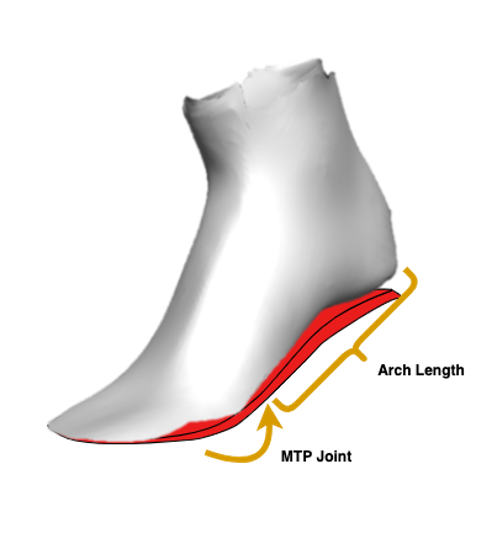
\includegraphics[width=0.5\textwidth,height=\textheight]{../fig/SA3/SoleFlex.png}
\caption{Desired sole flexibility (red) matched with plantar foot contour at MTP joint}\label{fig:SA3-SoleFlex}
}
\end{figure}

\hypertarget{framework-implementation}{%
\section{Framework Implementation}\label{framework-implementation}}

The presented framework outlines the integration of novel dynamic foot morphology data into the boot design process.
This process can help design a novel spacesuit boot that aims to both fit the foots shape and proper foot mobility, reducing the risk of injury and fit issues such as heel-lift.
Designing a spacesuit boot design from scratch rather than modifying existing terrestrial boots can ensure better fit and mobility, reducing the risk of injury.
The resulting boot design from this framework and corresponding computational analysis will serve as a starting point for iteration of a spacesuit boot prototype.

The spacesuit boot prototype will require construction with a pressure bladder for pressurization.
Heat-sealable urethane coated nylon (400D, Seattle Fabrics) will be used for the pressure bladder, which was recommended by spacesuit professionals.
Fabrication capabilities for the pressure bladder will be iteratively developed, starting with adding a pressure bladder to a terrestrial boot.
As design elements are finalized, they will integrated into prototype iterations.
When the design is finalized, a new boot will be constructed with all design elements.
A pressurization level of 3.5 psi will first be targeted, consistent with the operating pressure of the launch-entry-abort suits.
The final operating pressure will target 4.3 psi, the operating pressure of the EMU spacesuit.

The boot's design will use some existing, proven spacesuit construction techniques to ensure success.
The pressure bladder will be fixed to the inside of the shoe using a series of tabs, ensuring that it is always indexed properly inside the foot.
A convoluted joint will be used for ankle joint mobility, similar to \citep{Harris2001}.
The upper will act as a pressure restraint layer to prevent the pressure bladder from bellowing once pressurized.
Collaborations will be established with footwear design experts at the University of Oregon Portland to ensure the current art of footwear design in incorporated into the fabrication of the boot.
This ensures that the framework is implemented successfully in its translation into a spacesuit boot prototype.
An additional collaboration between CU and BOA Technologies may incorporate the use of BOA laces into the upper restraint layer to capture the midfoot.

The final design of the boot will aim to fit a range of individual foot measures.
As components of the boot are designed, the foot measure range they accommodate will be defined.
When all components are integrated into the final boot design, these foot measures will be used to recruit subjects who fit the boot; allowing for design evaluation in SA4.

\hypertarget{summary-4}{%
\section{Summary}\label{summary-4}}

This analysis outlined a framework for designing a new spacesuit boot with an emphasis on fit and mobility during gait.
The framework aims to reduce the risk of spacesuit boot injury by developing a process to design a spacesuit boot.
It is expected that focusing a design on fit and mobility will reduce the occurrence of heel-lift and contact injuries.

This framework therefore serves as bounding requirements to ensure future spacesuit footwear does not inhibit natural foot motion or cause discomfort due to incompatibilities between foot and shoe shape.
The only previously bounding requirement, the 2019 NASA SBIR solicitation for a new surface spacesuit boot, had only one requirement for ankle flexion/extension, which was validated in this paper.
There were no requirements other ankle motions or MTP join motions, and no requirement for proper static and dynamic fit to the wearer's foot.
This work provides a series of requirements based from previous biomechanics studies on foot motion while walking and hiking to provide proper fit and mobility through the spacesuit boot design.
Prototypes constructed from this work will be validated in Specific Aim 4.

As of Fall 2020, the literature review and biomechanical design framework have been completed.
Work is currently starting on the prototype spacesuit boot design and construction.
The literature review and biomechanical design framework have been presented in a paper published at the 2020 International Conference on Environmental Systems Meeting.
The final design of the boot will be presented in a future journal paper and conference presentations.

\hypertarget{specific-aim-4-evaluate-novel-planetary-spacesuit-boot-design-for-fit-comfort-and-mobility}{%
\chapter{Specific Aim 4: Evaluate novel planetary spacesuit boot design for fit, comfort, and mobility}\label{specific-aim-4-evaluate-novel-planetary-spacesuit-boot-design-for-fit-comfort-and-mobility}}

\hypertarget{introduction-3}{%
\section{Introduction}\label{introduction-3}}

The pressurized boot prototype developed in Specific Aim 3 will need to be validated to test the main hypothesis of this thesis: a spacesuit boot designed with dynamic foot morphology will provide increased compatibility between the spacesuit and operator.
The gold-standard of performance for EVA mobility would be an unpressurized hiking boot.
Current MK III boots feature only a convoluted ankle joint \citep{Ross2002}, which can be constructed as a pressurized hiking boot with a convoluted ankle joint.
The prototype will be compared against these two boot options, essentially testing the effects of boot pressurization with ankle mobility and the midfoot indexing feature designed in Specific Aim 3.
The prototype will be mated to a glovebox to allow for pressurized testing.
It is also desirable to test the prototype with subjects walking in the lab, which will require a shank-mounted pressure seal in place of a full spacesuit.
It may not be feasible to maintain this pressurized seal while subjects are ambulating.
Regardless of test-setup, the main objectives of this work are:

\begin{itemize}
\tightlist
\item
  Construct interface between test boots and test environments
\item
  Evaluate the mobility of the novel design against a standard hiking boot and pressurized hiking boot
\item
  Evaluate the comfort of the novel design against a standard hiking boot and pressurized hiking boot
\item
  Evaluate the novel design for its ability to reduce instances of heel lift against a standard hiking boot and pressurized hiking boot
\end{itemize}

\hypertarget{test-interface-construction}{%
\section{Test Interface Construction}\label{test-interface-construction}}

Interfaces will need to be constructed between the boots to be tested and the test environments, as shown in fig.~\ref{fig:SA4-interface} .
For the glovebox testing, the interface will need to allow for pressurization of the prototype boot and the MK III boot.
When a vacuum is pulled inside the glovebox, the boot will become pressurized with the ambient air.
The standard hiking boot will also need an interface to the glovebox to offer similar testing conditions, but will not need to be pressurized.

Another potential interface will be mate the pressurized boots to the shank of the wearer.
This interface will require some sort of seal above the wearer's ankle.
Due to expected imperfections in the seal, the boot will most likely be fed with constant pressurized air to maintain a constant pressure.
This interface will first be tested on the prototype iterations constructed in SA3 before being incorporated into the final prototype and pressurized hiking boot.

\begin{figure}
\hypertarget{fig:SA4-interface}{%
\centering
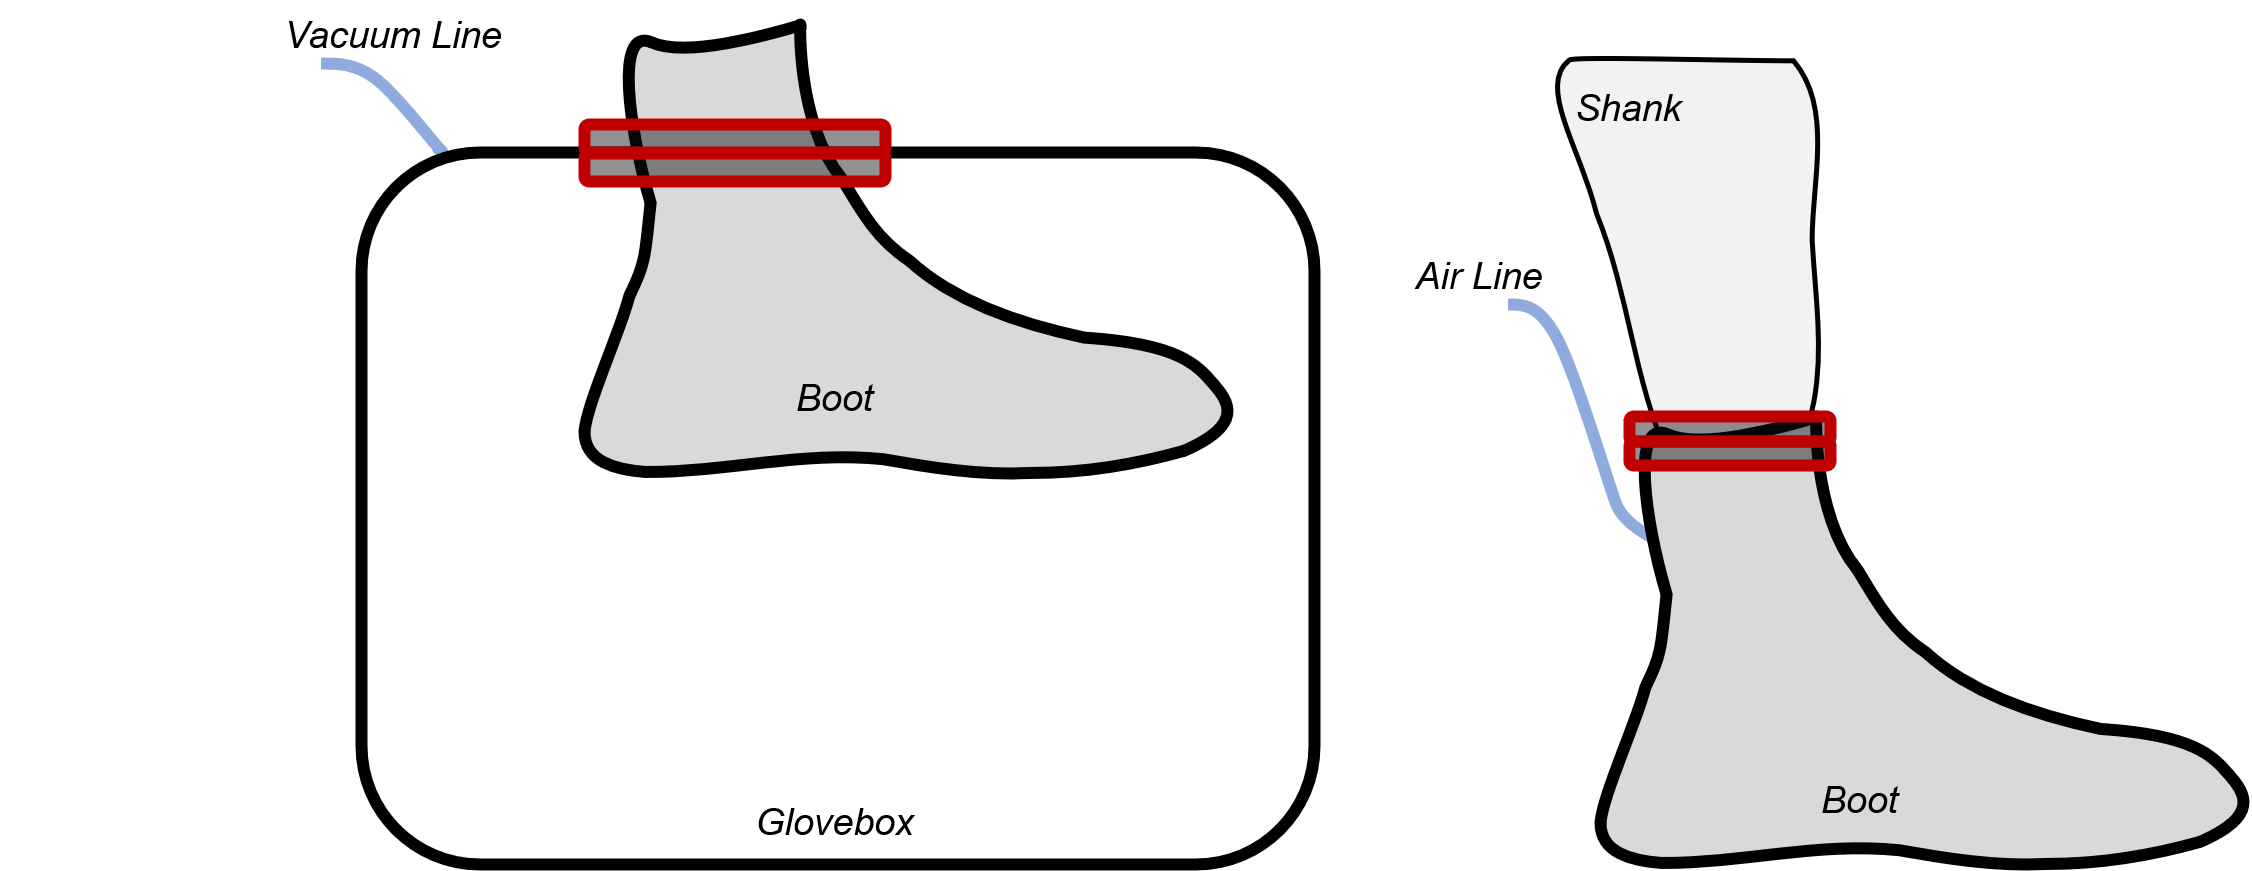
\includegraphics[width=1\textwidth,height=\textheight]{../fig/SA4/InterfaceDesign.png}
\caption{Two interface designs that will be prototyped in this thesis. (Left): Glovebox interface where a interface (red) connects the boot to the vacuum environment of the glovebox. (Right): Shank interface, where a seal (red) will be developed to tightly fit around the shank of the wearer, with a compressed air line entering the boot to pressurize it.}\label{fig:SA4-interface}
}
\end{figure}

\hypertarget{experimental-design-1}{%
\section{Experimental Design}\label{experimental-design-1}}

The hypotheses tested in this aim are as follows:

\begin{itemize}
\tightlist
\item
  The novel boot design will provide equivalent mobility compared to the standard hiking boot and improved mobility compared to the pressurized hiking boot
\item
  The novel boot design will provide equivalent comfort compared to the standard hiking boot and improved comfort compared to the pressurized hiking boot
\item
  The novel boot design will induce the same number of instances of heel lift as the hiking boot and fewer instances of heel lift compared to the pressurized hiking boot
\end{itemize}

The independent variables used to test these hypothesis will be the different boots tested: the standard hiking boot, the pressurized hiking boot (representing current planetary spacesuit boot technology), and the novel spacesuit boot developed in SA3.
The dependent variables tested will be the range-of-motion of the ankle joint, subjective survey results, and counts of heel-lift in a standardized trial.
Range-of-motion will be measured with photogrammetry, taken from the front and side profile, and used to assess mobility.
Subjective surveys will be provided to the subject to fill after finishing the range-of-motion tests.
The Corlett-Bishop Discomfort Scale \citep{Corlett1976}, Rating of Perceived Exertion Survey \citep{Borg1982}, and Gravity compensation and performance scale (GCPS) \citep{Gernhardt2009, Norcross2009, Norcross2010} will be used to assess subjective comfort of the boots.
Findings from Specific Aim 1 showed that IMUs may not be appropriate for detecting instances of heel-lift.
Therefore, a force sensor will be placed in the heel of the boot, in as minimally intrusive position as possible, to detect instances of heel-lift.
If possible, a sensor which can measure distance between the sole and heel will be selected for this application.
Instances of heel-lift will also be correlated to subjective comments, and future work may use the selected sensor to validate IMU usage in detecting heel-lift in the spacesuit.

Subjects will be recruited for this study whose feet fit the defined foot measure range of the novel spacesuit boot developed in SA3.
Subjects will be prescreened for their foot measures prior to being enrolled in the study.
A minimum of 5 subjects will be enrolled in this study.
The order in which a subject tests each boot will be counterbalanced to avoid carryover and fatigue effects.

All three boots will be mated to the glovebox, and a vacuum will be pulled for both pressurized boots to allow ambient air to pressurize them.
The glovebox will be placed on the ground, with the subject in a standing posture.
The subject will perform range-of-motion tests of their ankle inside the glovebox.
Motions will be performed both unloaded, where the boot is free in the air, and loaded, where the boot is pushing against a flat floor.
This is consistent with previous planetary boot testing methodology \citep{Ross2002}.
The subject will also perform a series of heel lifts to test for heel-lift.

\hypertarget{stretch-testing-goals}{%
\section{Stretch Testing Goals}\label{stretch-testing-goals}}

The glovebox testing will provide initial insight into comfort and mobility, but will be limited in translation as it does not include walking.
If a pressurized seal around the ankle is achievable, a biomechanical walking evaluation of the three boots can occur.
These evaluations will also be dependent on access to collaborators' lab facilities with force plates and optical motion capture.
The boot will be pressurized through a portable compressor, with a pressure line running to the subject and routed to the boot.
The stated hypotheses and independent variables will remain the same for walking testing, but joint torques will be added as a dependent variable.

Walking will occur on a flat walkway, where the subject will walk across force plates to measure ground reaction forces.
Optical motion capture will be used to capture segment kinematics of the lower torso, allowing for calculation of joint range-of-motions for mobility assessment.
A kinetic analysis from the kinematics and ground reaction forces can provide information on joint torques at the ankle, knee, and pelvis.
The aforementioned subjective surveys will be administered following data collection with each boot.

Suited testing will be pursued through collaborators at David Clark or NASA Johnson Space Center.
If spacesuit access is granted, the prototype will be integrated into the spacesuit through an ankle bearing assembly.
Testing procedures will mirror those described previously with walking tests.

\hypertarget{summary-5}{%
\section{Summary}\label{summary-5}}

This work will evaluate the fit and mobility of the boot designed in Specific Aim 3.
Results from this work will directly inform the performance of a boot designed with body-shape modeling techniques.
This work will not be started until Specific Aim 3 is complete, as it depends on the delivery of the prototype boot.

\hypertarget{summary-and-execution-plan}{%
\chapter{Summary and Execution Plan}\label{summary-and-execution-plan}}

Through many advancements of planetary EVA spacesuit design, operator-spacesuit coordination is still not perfectly matched.
Poor mobility and poor fit between the operator and spacesuit are some of the most common factors that can lead to injury.
This thesis aims to determine the feasibility of using dynamic body shape models to improve spacesuit component fit and mobility, specifically with planetary spacesuit boots.
The spacesuit boot has demonstrated specific problems relating to poor fit, such as heel-lift and contact injuries.
The work in the thesis aims to answer the hypothesis:

\begin{quote}
Integrating dynamic body shape changes into the spacesuit boot design process will mitigate factors that lead to injury and improve compatibility between the operator and the spacesuit.
\end{quote}

To date, the following contributions have been completed:

\begin{itemize}
\tightlist
\item
  Showed drawbacks and identified areas of future implementation for how IMUs could be used to detect instances of heel-lift
\item
  A novel software library to use multiple commercial depth cameras as a cost-effective 4D scanner, capable of collecting body shape changes at 90 frames-per-second
\item
  A parametric statistical shape model that predicts dynamic foot shape during stance phase as a function of anthropometry and kinematics
\item
  A design framework integrating dynamic foot shape knowledge with known foot mobility to design a novel spacesuit boot to improve fit and comfort
\end{itemize}

This thesis aims to provide the following contributions during the remainder of its course:

\begin{itemize}
\tightlist
\item
  Quantification of dynamic changes in instep height and instep girth as they relate to their distribution in the global population
\item
  A novel spacesuit boot prototype developed from the framework that aims for better fit and comfort, and specifically a reduction in heel-lift
\item
  Evaluation of the novel spacesuit boot for comfort and mobility against current planetary spacesuit boot technology and a gold-standard hiking boot
\end{itemize}

Through these contributions, this thesis aims to show the efficacy of dynamic body-shape models in improving spacesuit component design for fit, comfort, and mobility, thereby answering its hypothesis.
While the efforts of this thesis were demonstrated on a planetary spacesuit boot, the presented work aims to serve as a foundation for other spacesuit component designs where fit may be an issue, such as the HUT and gloves.
The work presented in this thesis also aims to be translational for terrestrial footwear, contributing a new capture tool and modeling technique to improve footwear fit and comfort for a variety of activities.

\hypertarget{publication-plan}{%
\section{Publication Plan}\label{publication-plan}}

Table \ref{tbl:pubs} outlines the peer-reviewed conference and journal papers from this thesis work.
Table \ref{tbl:conf} outlines conference presentations and posters from this thesis work.
Publications and presentations which are proposed and subject to having their title changed.

\pagebreak

\hypertarget{tbl:pubs}{}
\begin{longtable}[]{@{}llll@{}}
\caption{\label{tbl:pubs}Peer-reviewed publications}\tabularnewline
\toprule
\begin{minipage}[b]{0.09\columnwidth}\raggedright
Type\strut
\end{minipage} & \begin{minipage}[b]{0.35\columnwidth}\raggedright
Title\strut
\end{minipage} & \begin{minipage}[b]{0.27\columnwidth}\raggedright
Journal\strut
\end{minipage} & \begin{minipage}[b]{0.18\columnwidth}\raggedright
Status\strut
\end{minipage}\tabularnewline
\midrule
\endfirsthead
\toprule
\begin{minipage}[b]{0.09\columnwidth}\raggedright
Type\strut
\end{minipage} & \begin{minipage}[b]{0.35\columnwidth}\raggedright
Title\strut
\end{minipage} & \begin{minipage}[b]{0.27\columnwidth}\raggedright
Journal\strut
\end{minipage} & \begin{minipage}[b]{0.18\columnwidth}\raggedright
Status\strut
\end{minipage}\tabularnewline
\midrule
\endhead
\begin{minipage}[t]{0.09\columnwidth}\raggedright
Technical Note\strut
\end{minipage} & \begin{minipage}[t]{0.35\columnwidth}\raggedright
Detecting Heel-Lift in Spacesuit Gait\strut
\end{minipage} & \begin{minipage}[t]{0.27\columnwidth}\raggedright
Aerospace Medicine and Human Performance\strut
\end{minipage} & \begin{minipage}[t]{0.18\columnwidth}\raggedright
In Prep., expected Nov 2020\strut
\end{minipage}\tabularnewline
\begin{minipage}[t]{0.09\columnwidth}\raggedright
\strut
\end{minipage} & \begin{minipage}[t]{0.35\columnwidth}\raggedright
\strut
\end{minipage} & \begin{minipage}[t]{0.27\columnwidth}\raggedright
\strut
\end{minipage} & \begin{minipage}[t]{0.18\columnwidth}\raggedright
\strut
\end{minipage}\tabularnewline
\begin{minipage}[t]{0.09\columnwidth}\raggedright
Journal Paper\strut
\end{minipage} & \begin{minipage}[t]{0.35\columnwidth}\raggedright
DynaMo: Dynamic Body Shape and Motion Capture with Intel RealSense Cameras\strut
\end{minipage} & \begin{minipage}[t]{0.27\columnwidth}\raggedright
Journal of Open Source Software\strut
\end{minipage} & \begin{minipage}[t]{0.18\columnwidth}\raggedright
Published\strut
\end{minipage}\tabularnewline
\begin{minipage}[t]{0.09\columnwidth}\raggedright
\strut
\end{minipage} & \begin{minipage}[t]{0.35\columnwidth}\raggedright
\strut
\end{minipage} & \begin{minipage}[t]{0.27\columnwidth}\raggedright
\strut
\end{minipage} & \begin{minipage}[t]{0.18\columnwidth}\raggedright
\strut
\end{minipage}\tabularnewline
\begin{minipage}[t]{0.09\columnwidth}\raggedright
Journal Paper\strut
\end{minipage} & \begin{minipage}[t]{0.35\columnwidth}\raggedright
Dynamic foot morphology explained through 4D scanning and shape modeling\strut
\end{minipage} & \begin{minipage}[t]{0.27\columnwidth}\raggedright
Journal of Biomechanics\strut
\end{minipage} & \begin{minipage}[t]{0.18\columnwidth}\raggedright
Under Review\strut
\end{minipage}\tabularnewline
\begin{minipage}[t]{0.09\columnwidth}\raggedright
\strut
\end{minipage} & \begin{minipage}[t]{0.35\columnwidth}\raggedright
\strut
\end{minipage} & \begin{minipage}[t]{0.27\columnwidth}\raggedright
\strut
\end{minipage} & \begin{minipage}[t]{0.18\columnwidth}\raggedright
\strut
\end{minipage}\tabularnewline
\begin{minipage}[t]{0.09\columnwidth}\raggedright
Conference Paper\strut
\end{minipage} & \begin{minipage}[t]{0.35\columnwidth}\raggedright
A Biomechanical Design Framework to Improve Spacesuit Boot Fit\strut
\end{minipage} & \begin{minipage}[t]{0.27\columnwidth}\raggedright
50th International Conference on Environmental Systems\strut
\end{minipage} & \begin{minipage}[t]{0.18\columnwidth}\raggedright
Published\strut
\end{minipage}\tabularnewline
\begin{minipage}[t]{0.09\columnwidth}\raggedright
\strut
\end{minipage} & \begin{minipage}[t]{0.35\columnwidth}\raggedright
\strut
\end{minipage} & \begin{minipage}[t]{0.27\columnwidth}\raggedright
\strut
\end{minipage} & \begin{minipage}[t]{0.18\columnwidth}\raggedright
\strut
\end{minipage}\tabularnewline
\begin{minipage}[t]{0.09\columnwidth}\raggedright
Journal Paper\strut
\end{minipage} & \begin{minipage}[t]{0.35\columnwidth}\raggedright
Static and Dynamic Distribution of Instep Height\strut
\end{minipage} & \begin{minipage}[t]{0.27\columnwidth}\raggedright
Footwear Science\strut
\end{minipage} & \begin{minipage}[t]{0.18\columnwidth}\raggedright
Proposed, expected Mar 2021\strut
\end{minipage}\tabularnewline
\begin{minipage}[t]{0.09\columnwidth}\raggedright
\strut
\end{minipage} & \begin{minipage}[t]{0.35\columnwidth}\raggedright
\strut
\end{minipage} & \begin{minipage}[t]{0.27\columnwidth}\raggedright
\strut
\end{minipage} & \begin{minipage}[t]{0.18\columnwidth}\raggedright
\strut
\end{minipage}\tabularnewline
\begin{minipage}[t]{0.09\columnwidth}\raggedright
Journal Paper\strut
\end{minipage} & \begin{minipage}[t]{0.35\columnwidth}\raggedright
Design of A Novel Planetary Spacesuit Boot Design\strut
\end{minipage} & \begin{minipage}[t]{0.27\columnwidth}\raggedright
Acta Astronautica\strut
\end{minipage} & \begin{minipage}[t]{0.18\columnwidth}\raggedright
Proposed, expected Aug 2021\strut
\end{minipage}\tabularnewline
\begin{minipage}[t]{0.09\columnwidth}\raggedright
\strut
\end{minipage} & \begin{minipage}[t]{0.35\columnwidth}\raggedright
\strut
\end{minipage} & \begin{minipage}[t]{0.27\columnwidth}\raggedright
\strut
\end{minipage} & \begin{minipage}[t]{0.18\columnwidth}\raggedright
\strut
\end{minipage}\tabularnewline
\begin{minipage}[t]{0.09\columnwidth}\raggedright
Journal Paper\strut
\end{minipage} & \begin{minipage}[t]{0.35\columnwidth}\raggedright
Comfort and Mobility Evaluation of a Novel Planetary Spacesuit Boot Design\strut
\end{minipage} & \begin{minipage}[t]{0.27\columnwidth}\raggedright
Aerospace Medicine and Human Performance\strut
\end{minipage} & \begin{minipage}[t]{0.18\columnwidth}\raggedright
Proposed, expected Feb 2022\strut
\end{minipage}\tabularnewline
\bottomrule
\end{longtable}

\pagebreak

\hypertarget{tbl:conf}{}
\begin{longtable}[]{@{}llll@{}}
\caption{\label{tbl:conf}Conference Presentations and Posters}\tabularnewline
\toprule
\begin{minipage}[b]{0.11\columnwidth}\raggedright
Type\strut
\end{minipage} & \begin{minipage}[b]{0.44\columnwidth}\raggedright
Title\strut
\end{minipage} & \begin{minipage}[b]{0.22\columnwidth}\raggedright
Conference\strut
\end{minipage} & \begin{minipage}[b]{0.11\columnwidth}\raggedright
Date\strut
\end{minipage}\tabularnewline
\midrule
\endfirsthead
\toprule
\begin{minipage}[b]{0.11\columnwidth}\raggedright
Type\strut
\end{minipage} & \begin{minipage}[b]{0.44\columnwidth}\raggedright
Title\strut
\end{minipage} & \begin{minipage}[b]{0.22\columnwidth}\raggedright
Conference\strut
\end{minipage} & \begin{minipage}[b]{0.11\columnwidth}\raggedright
Date\strut
\end{minipage}\tabularnewline
\midrule
\endhead
\begin{minipage}[t]{0.11\columnwidth}\raggedright
Talk\strut
\end{minipage} & \begin{minipage}[t]{0.44\columnwidth}\raggedright
Using dynamic foot morphology data to design spacesuit footwear\strut
\end{minipage} & \begin{minipage}[t]{0.22\columnwidth}\raggedright
Footwear Biomechanics Symposium\strut
\end{minipage} & \begin{minipage}[t]{0.11\columnwidth}\raggedright
July 2019\strut
\end{minipage}\tabularnewline
\begin{minipage}[t]{0.11\columnwidth}\raggedright
\strut
\end{minipage} & \begin{minipage}[t]{0.44\columnwidth}\raggedright
\strut
\end{minipage} & \begin{minipage}[t]{0.22\columnwidth}\raggedright
\strut
\end{minipage} & \begin{minipage}[t]{0.11\columnwidth}\raggedright
\strut
\end{minipage}\tabularnewline
\begin{minipage}[t]{0.11\columnwidth}\raggedright
Talk\strut
\end{minipage} & \begin{minipage}[t]{0.44\columnwidth}\raggedright
Development of a Dynamic 3D Scanning System with Multiple Intel RealSense Depth Cameras\strut
\end{minipage} & \begin{minipage}[t]{0.22\columnwidth}\raggedright
International Society of Biomechanics Congress\strut
\end{minipage} & \begin{minipage}[t]{0.11\columnwidth}\raggedright
Aug 2019\strut
\end{minipage}\tabularnewline
\begin{minipage}[t]{0.11\columnwidth}\raggedright
\strut
\end{minipage} & \begin{minipage}[t]{0.44\columnwidth}\raggedright
\strut
\end{minipage} & \begin{minipage}[t]{0.22\columnwidth}\raggedright
\strut
\end{minipage} & \begin{minipage}[t]{0.11\columnwidth}\raggedright
\strut
\end{minipage}\tabularnewline
\begin{minipage}[t]{0.11\columnwidth}\raggedright
Poster\strut
\end{minipage} & \begin{minipage}[t]{0.44\columnwidth}\raggedright
Quantifying the Heel-Lift during Spacesuit Gait\strut
\end{minipage} & \begin{minipage}[t]{0.22\columnwidth}\raggedright
NASA HRP IWS\strut
\end{minipage} & \begin{minipage}[t]{0.11\columnwidth}\raggedright
Jan 2020\strut
\end{minipage}\tabularnewline
\begin{minipage}[t]{0.11\columnwidth}\raggedright
\strut
\end{minipage} & \begin{minipage}[t]{0.44\columnwidth}\raggedright
\strut
\end{minipage} & \begin{minipage}[t]{0.22\columnwidth}\raggedright
\strut
\end{minipage} & \begin{minipage}[t]{0.11\columnwidth}\raggedright
\strut
\end{minipage}\tabularnewline
\begin{minipage}[t]{0.11\columnwidth}\raggedright
TBD\strut
\end{minipage} & \begin{minipage}[t]{0.44\columnwidth}\raggedright
Dynamic Body-Shape Models to Reduce Risk OF EVA Spacesuit Injury\strut
\end{minipage} & \begin{minipage}[t]{0.22\columnwidth}\raggedright
NASA HRP IWS\strut
\end{minipage} & \begin{minipage}[t]{0.11\columnwidth}\raggedright
Feb 2021\strut
\end{minipage}\tabularnewline
\begin{minipage}[t]{0.11\columnwidth}\raggedright
\strut
\end{minipage} & \begin{minipage}[t]{0.44\columnwidth}\raggedright
\strut
\end{minipage} & \begin{minipage}[t]{0.22\columnwidth}\raggedright
\strut
\end{minipage} & \begin{minipage}[t]{0.11\columnwidth}\raggedright
\strut
\end{minipage}\tabularnewline
\begin{minipage}[t]{0.11\columnwidth}\raggedright
TBD\strut
\end{minipage} & \begin{minipage}[t]{0.44\columnwidth}\raggedright
Novel Spacesuit Boot Design Developed from Dynamic Foot Shape Modeling\strut
\end{minipage} & \begin{minipage}[t]{0.22\columnwidth}\raggedright
Footwear Biomechanics Symposium\strut
\end{minipage} & \begin{minipage}[t]{0.11\columnwidth}\raggedright
July 2021\strut
\end{minipage}\tabularnewline
\begin{minipage}[t]{0.11\columnwidth}\raggedright
\strut
\end{minipage} & \begin{minipage}[t]{0.44\columnwidth}\raggedright
\strut
\end{minipage} & \begin{minipage}[t]{0.22\columnwidth}\raggedright
\strut
\end{minipage} & \begin{minipage}[t]{0.11\columnwidth}\raggedright
\strut
\end{minipage}\tabularnewline
\begin{minipage}[t]{0.11\columnwidth}\raggedright
TBD\strut
\end{minipage} & \begin{minipage}[t]{0.44\columnwidth}\raggedright
Spacesuit Boot with Improved Comfort and Mobility Developed from Dynamic Shape Modeling\strut
\end{minipage} & \begin{minipage}[t]{0.22\columnwidth}\raggedright
NASA HRP IWS\strut
\end{minipage} & \begin{minipage}[t]{0.11\columnwidth}\raggedright
Jan 2022\strut
\end{minipage}\tabularnewline
\bottomrule
\end{longtable}

\hypertarget{academic-requirements}{%
\section{Academic Requirements}\label{academic-requirements}}

All required coursework was completed as of the Spring 2020 semester. Of the 36 required credits, 30 were taken in ASEN, with 12 at the 6000 level. MCEN 5228 (Modeling Human Movement) and APPM 5590 (Statistical Modeling) were taken outside of ASEN. The 6 required math credits were exceeded with taking ASEN 5519 (Experimental Design and Statistical Analysis), APPM 5590 (Statistical Modeling), and ASEN 5044 (Statistical Estimation for Dynamical Systems). As of the Fall 2020 semester, 15 out of the 30 required Doctoral dissertation credits have been taken. The remaining 15 credits will be evenly taken during the Spring 2021, Fall 2021, and Spring 2022 semesters. The teaching practicum has been fulfilled through the mentoring of UROP students in the Summer 2018, Fall 2019, and Spring 2020 semesters. A TA position is also expected in Fall 2021.

\hypertarget{timeline}{%
\section{Timeline}\label{timeline}}

Gantt chart \ref{fig:Gantt} shows the timeline for each specific aim of the thesis and for PhD graduation milestones.

\begin{figure}
\hypertarget{fig:Gantt}{%
\centering
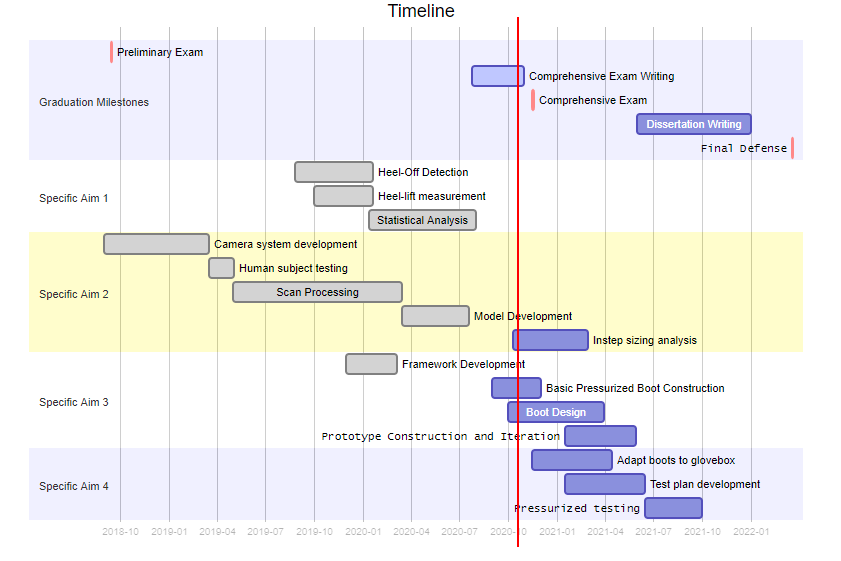
\includegraphics[width=1\textwidth,height=\textheight]{../fig/Gantt.png}
\caption{Gantt chart showing PhD timeline}\label{fig:Gantt}
}
\end{figure}

%%%%%%%%%   then the Bibliography, if any   %%%%%%%%%
%\bibliographystyle{plain}	% or "siam", or "alpha", etc.
%\nocite{*}		% list all refs in database, cited or not
%\bibliography{refs}		% Bib database in "refs.bib"

%%%%%%%%%   then the Appendices, if any   %%%%%%%%%
%%\appendix
\newpage


%\usepackage{natbib}
\bibliography{../references}



\end{document}
